% Autor: Adina Wagner, 215486

%---------- Pakete und Dokumenteinstellungen -------------------------------------

\documentclass[a4paper, 11pt]{scrreprt}

\usepackage[ngerman, american]{babel}   %andersherum, also "ngerman, american" sind die Ueberschriften in Englisch
\usepackage[T1]{fontenc}			%Kodierung des Zeichensatzes
\usepackage[utf8]{inputenc}		%Dt. Umlaute mit Schriftsatz
%\usepackage[latin1]{inputenc}
\usepackage[a4paper, left=2.5cm, right=2.5cm, top=3cm, bottom=3cm]{geometry}
\usepackage{latexsym}
\usepackage{amsmath}		% Mathe-Paket
\usepackage{amsthm}
\usepackage{graphicx}		% Paket für Graphiken
\usepackage{color,psfrag}
\usepackage{amssymb}		% spez. Mathe-Symbole
\usepackage{dsfont}
\usepackage{framed, color}
\usepackage[automark,headsepline]{scrpage2}
\usepackage{eurosym}		% Euro-Zeichen Symbol via \euro, bzw. \EUR{x,yz} liefert x,yz €
\usepackage{leftidx}
\usepackage{longtable}
\usepackage{array}
\usepackage{stmaryrd}		%Widerspruchsblitz via \lightning
\usepackage{enumitem} %Anpassbare Enumerates/Itemizes
\usepackage{trfsigns} % \e, \im
\usepackage{dlfltxbcodetips }	%\bigtimes
\usepackage{rotating} 	% Tabellen im Querformat
\usepackage{floatrow} % Caption neben Abbildungen
% \usepackage{makecell} % dicke Linien in Tabellen
%\usepackage{setspace}

\usepackage[toc,page]{appendix}	% Anhang

\usepackage[linesnumbered, ruled]{algorithm2e}	% Algorithmus
\usepackage{listings}	% Code einbinden, aufrufen mit \lstinputlisting{source_filename.py}


\automark[section]{chapter}	%setzt Seitenüberschriften

\geometry{	left=30mm,			%innerer Seitenrand
			top=25mm,				%Seitenoberkante
			width=155mm,			%Textbreite
			height=247mm,			%Texthöhe
			marginparsep=5mm,		%Abstand Notizrand
			marginparwidth=20mm		%Breite Notizrand
		}
		
%------------Abbildungen-----------------------------------------------

\usepackage{graphicx}					%Einbinden von Bildern
\usepackage{calc}						%Berechnen von Längen
\usepackage{float}						%Abb.& Tabellen exakt einbinden mit [H]-Zusatz
\usepackage{subfigure}					%Subfigures mehrere Bilder nebeneinander

\usepackage[format=hang, justification=justified]{caption}	%Bildunterschrift

\newcolumntype{C}[1]{>{\centering\arraybackslash}m{#1}} %zentrierte Spalten mit fester Breite

% Spezialpakete für tikzpicture
\usepackage{fp}
\usepackage{tikz}
\usepackage{xcolor}
\usepackage{pgfplots}

% TikZ-Bibliotheken
\usetikzlibrary{arrows}
\usetikzlibrary{shapes}
\usetikzlibrary{decorations.pathmorphing}
\usetikzlibrary{decorations.pathreplacing}
\usetikzlibrary{decorations.shapes}
\usetikzlibrary{decorations.text}


%\usepackage{scrpage2}
\pagestyle{scrheadings}			

%\clearscrheadings	
%\clearscrplain		
\clearscrheadfoot
\ihead[]{\leftmark}						%setzt Chapter-Name als linke Seitenüberschrift
\ohead[]{***DRAFT*** v.0.1 DEC 2018} 				%für sectionname \rightmark einsetzen
%\cfoot[\pagemark]{\pagemark}
\cfoot[\hfill -- \thepage{} -- \hfill]{\hfill -- \thepage{} -- \hfill}	%setzt Seitenzahl unten
\setkomafont{pagefoot}{%
\normalfont\sffamily}

\linespread{1.1} 						%Zeilenabstand
\setlength{\parindent}{0cm} 	%keine Einzüge

\setlength{\unitlength}{3ex}		% Längengrundeinheit auf 3-fache Höhe von "x" setzen.

% dicke Linien in Tabellen: \thickhline 

\makeatletter
\def\thickhline{%
	\noalign{\ifnum0=`}\fi\hrule \@height \thickarrayrulewidth \futurelet
	\reserved@a\@xthickhline}
\def\@xthickhline{\ifx\reserved@a\thickhline
	\vskip\doublerulesep
	\vskip-\thickarrayrulewidth
	\fi
	\ifnum0=`{\fi}}
\makeatother

\newlength{\thickarrayrulewidth}
\setlength{\thickarrayrulewidth}{4\arrayrulewidth} % hier Dicke einstellen


%------------ Eigene Definitionen und Befehle -----------------------------

\newtheorem{Theorem}{Theorem}[chapter]
\newtheorem{Lemma}[Theorem]{Lemma}
\newtheorem{Cor}[Theorem]{Corollary}
\newtheorem{Prop}[Theorem]{Proposition}
\newtheorem{Code}[Theorem]{Code}
\newtheorem{Assumption}[Theorem]{Assumption}
\newtheorem{Construction}[Theorem]{Construction}
\newtheorem{Motivation}[Theorem]{Motivation}
\newtheorem{Def}[Theorem]{Definition}
\newtheorem{Remark}[Theorem]{Remark}
\newtheorem{Ex}[Theorem]{Example}
\def\ci{\perp\!\!\!\perp} %stochastisch unabhängig
\newcommand{\RR}{\mathbb{R}}
\newcommand{\Rquer}{\overline\RR} 
\newcommand{\Null}{{\mathrm{Null}}}
\newcommand{\Range}{{\mathrm{Range}}}
\newcommand{\trace}{{\mathrm{trace}}}
\newcommand{\diag}{{\mathrm{diag}}}
\newcommand{\rank}{{\mathrm{rank}}}
\newcommand{\mm}{{\mathrm{m}}}
\newcommand{\supp}{{\mathrm{supp}}}
\newcommand{\logit}{\mathrm{logit}}
\newcommand{\odds}{\mathrm{odds}}
\newcommand{\qede}{\qquad \hfill \fbox{}}

\newcommand{\ind}{\mathbb{1}_}
\newcommand{\ew}{\mbox{\textbf{E}}}
\newcommand{\var}{\mbox{\textbf{Var}}}
\newcommand{\cov}{\mbox{\textbf{Cov}}}
\newcommand{\cor}{\mbox{\textbf{Corr}}}
\newcommand{\FF}{\mathfrak{F}}
\newcommand{\NN}{\mathbb{N}_0}
\newcommand{\PP}{\mathbb{P}}
\newcommand{\TT}{\mathfrak{T}}
\newcommand{\wra}{$(\Omega,\mathcal{F},\PP)$ }
\newcommand{\mc}{\multicolumn{2}{l}}
\newcommand{\nn}{\nonumber}
\newcommand{\bs}{\begin{upshape}}
\newcommand{\es}{\end{upshape}}
\newcommand{\norm}{\|}

\newcommand*{\discup}{\cup \hspace{-1.6ex} \cdot \hspace{0.6ex}}


\renewcommand{\labelitemii}{$\bullet$}
\renewcommand{\arraystretch}{1.0}
\renewcommand{\tablename}{\normalsize Table:}
\renewcommand{\im}{\mathrm{i}}
%\setheadsepline{0.4pt}
\setcounter{tocdepth}{2}

%------------Literaturverzeichnis--------

\usepackage[babel,german=quotes]{csquotes}
\usepackage[	style=authoryear,		% oder numeric
							backend=bibtex,			% oder biber
%							firstinits=true,		% Vorname abgekürzt
							maxitems= 12				% maximale Anzahl an Authoren, Abkürzung et alter
						]{biblatex}
\renewbibmacro{in:}{} 	% unterdrücke "in:" vor dem Journal-Titel						
\renewcommand*{\mkbibnamelast}[1]{\textsc{#1}} 	% Autoren in Kapitälchen
\setlength{\bibhang}{2em}		% hängender Einzug
						
\addbibresource{Literatur.bib}			% Pfad zur Datei im selben Ordner




% --------- Abkürzungsverzeichnis ------------------
\usepackage{nomencl}	% Package für Abkürzungsverzeichnis
\setlength{\nomitemsep}{-\parsep} % Zeilenabstand 
\setlength{\nomlabelwidth}{.15\hsize}	% Erklärungen bündig
\makenomenclature
%%% Ausführen in der Konsole

% D:
% cd STUDIUM\_Master\Masterabeit\LaTeX\LaTeX aktuell
% makeindex Masterarbeit.nlo -s nomencl.ist -o Masterarbeit.nls


% ---------------- Dokument ----------------------

\begin{document}

% ------------ Deckblatt --------------------------

\begin{figure}[h]
\vspace{-1.5cm}
\hspace{9.5cm}

\includegraphics[scale=0.5]{img/ovgu_nat_logo}
\label{logoOVGU}
\end{figure}

\begin{center}
\bigskip
\begin{LARGE}
\textbf{Masters' Thesis}
\end{LARGE}

\vspace{\fill}

\begin{huge}
%\begin{scshape}
 
\textbf{Catching the eye}: \\
Investigating the functional neuroanatomy of the visuospatial attention system with fMRI and eyegaze recordings during natural stimulation

%\end{scshape}
\end{huge}

\vspace{\fill}

submitted by\\
\begin{large}
Adina Wagner (215486) \\
\vspace{0.3cm}
Master of Science in Clinical Neuroscience\\
\begin{normalsize}
adina.wagner@t-online.de 
\end{normalsize}

\vspace{\fill}

\begin{normalsize}
submitted to\\
\end{normalsize}
J.-Prof. Dr. Michael Hanke\\
Prof. Dr. Stefan Pollmann\\
\vspace{0.5cm}
Psychoinformatics Lab\\
Otto-von-Guericke Universität Magdeburg\\
\end{large}

\vspace{1cm}

February $3^{rd}$, 2019

\thispagestyle{empty}
\end{center}
\clearpage


% -------- Ende Deckblatt ----------------------

% ------- Leere Seite nach dem Deckblatt -------
%\newpage 
%\thispagestyle{empty}
%$\phantom{.}$
%\clearpage


%---- Eigenständigkeitserklärung -----------------


\chapter*{Statutory Declaration}
\addcontentsline{toc}{section}{Statutory Declaration}

I declare that I have authored this thesis independently, that I have not used
other than the declared sources/resources, and that I have explicitly marked
all material which has been quoted either literally or by content from the
used sources.

\bigskip

\begin{center}
	***
\end{center}

\bigskip

Hiermit versichere ich, dass ich die vorliegende Arbeit selbständig und nur
unter Benutzung der angegebenen Literatur- und Hilfsmittel angefertigt
habe. Wörtlich übernommene Sätze und Satzteile aus anderen Druckwerken
oder aus Internetpublikationen sind als Zitat belegt, andere Anlehnungen
hinsichtlich Aussage und Umfang unter Angabe der Quelle kenntlich gemacht.
Die Arbeit wurde in gleicher oder ähnlicher Form in keiner anderen
Lehrveranstaltung als Leistungsnachweis eingereicht.
Ich bin darüber unterrichtet, dass die Lehrenden angewiesen sind, schriftliche
 Arbeiten zu überprüfen, und dass ein Vergehen eine Meldung beim
Prüfungsausschuss der Fakultät zur Folge hat, die im schlimmsten Fall zum
Ausschluss aus der Universität führen kann.

\bigskip

\begin{center}
	***
\end{center}

\bigskip

Magdeburg, February $3^{rd}$, 2019

\bigskip

\bigskip

\bigskip

---------------------------------------------------

$\phantom{mmmm..}$  (Adina Wagner)

\clearpage


% ------- Schlauer Spruch --------------------
\chapter*{ }

\renewenvironment{quote}
	{\list{}{\rightmargin=1cm \leftmargin=5cm} %
		\item \relax}
	{\endlist}

\begin{quote}
\textit{The cure for boredom is curiosity. There is no cure for curiosity.}

\medskip
-- Ellen Parr 
\end{quote}


\clearpage

% ------- Inhaltsverzeichnis ------------------
\addcontentsline{toc}{section}{Table of Contents}
\tableofcontents

% ---------- Abbildungsverzeichnis -------------
\clearpage
\addcontentsline{toc}{section}{List of Figures}
\listoffigures
\clearpage

\addcontentsline{toc}{section}{List of Tables}
\listoftables
\clearpage

\addcontentsline{toc}{section}{List of Algorithms}
\listofalgorithms
\clearpage

% ---------- Abkürzungsverzeichnis -------------
\clearpage
\addcontentsline{toc}{section}{Nomenclature}
\printnomenclature

\nomenclature{FFA}{Fusiform Face Area}
\nomenclature{EBA}{Extrastriate Body Area}
\nomenclature{PPA}{Parahippocampal Place Area}
\nomenclature{LOC}{}
\nomenclature{fMRI}{functional Magnetic Resonance Imaging}
\nomenclature{PET}{Positron Emission Tomography}
\nomenclature{}{}
\nomenclature{}{}
\nomenclature{}{}
\nomenclature{}{}
\nomenclature{}{}
\nomenclature{}{}
\nomenclature{}{}
\nomenclature{}{}
\nomenclature{}{}
\nomenclature{MF}{Magnification Factor}
\nomenclature{}{}
\nomenclature{}{}
\nomenclature{GLM}{General linear model}
\nomenclature{OLS}{ordinary least-squares}
\nomenclature{SSE}{explained sum of squares}
\nomenclature{SSR}{residual sum of squares}
\nomenclature{SST}{total sum of squares}
\nomenclature{AR}{autoregressive process}
\nomenclature{MSE}{mean squared error}



\clearpage


%---------- Acknowledgments -------------

\chapter*{Acknowledgements}
\addcontentsline{toc}{section}{Acknowledgements}

I am thankful to a large number of people who supported and challenged me on the path of my master thesis completion and beyond. First and most important of all, I would like to thank my scientific supervisor J.-Prof. Dr. Michael Hanke of the Psychoinformatics Lab. He introduced me to the mesmerizing field of Psychoinformatics and has provided me with more opportunities I can recall to take root in it. A list of things that would not have been possible without him would span pages. I attribute much of my personal growth and scientific advancement of the past 1.5 years to him, and I am very grateful to continue pursuing my academic career as a PhD student under his supervision. \newline
Secondly, I am grateful to Prof. Dr. Pollmann for agreeing to be the second assessor of my Masters Thesis, and for valuable discussions and insights with regard to the thesis.\newline
I cannot overstate the importance of Prof. Yaroslav Halchenko, whom I want to thank deeply for his agreement to supervise and mentor me on a four month research stay at Jim Haxbys Lab at Dartmouth College, NH, USA. His and Michaels passion for open science, open-source software, and scientific integrity and reproducibility will continue to be my source of inspiration and motivation throughout my scientific career.\newline
I further am grateful to Prof. Jim Haxby for welcoming me in his lab in Dartmouth, as well as Prof. Ida Gobbini, Vassiki Chauhan, Kyle Meyer and Feilong Ma for their company and advice throughout my stay in the US. \newline
This Masters Thesis would not have been possible without the methodological discussions, programming tutorials, and most importantly friendship of Alexander Waite, Dr. Emanuele Porcu, Benjamin Poldrack, Christian Häusler and Asim Dar. All members of the Psychoinformatics Lab have contributed to the most welcoming, fun, and empowering work environment I have ever been a part of, and despite my daily commute, this wonderful lab became a family for me. \newline
All of my studies, in Germany and abroad, were mainly funded by the German Academic Foundation. The ideal and financial support since 2013 enabled me to become the person I am today. I am thankful to all of my referees, Dr. Ludwig, Dr. Trebesius, Dr. Köhne, and Dr. Chwalleck, for the insightful discussions, and my mentors, Prof. Enders and Prof. Fink, for their assistance and guidance, and to Dr. Julius and Prof. Zimmermann, whom I was honored to meet and work with several times. \newline
Last but not least I am heartily grateful to my parents and friends for their patience, their support, their steady encouragement and constant moral guidance. Especially Gunnar Behrens, who was my anchor throughout seven busy years.


\clearpage

\pagenumbering{arabic}
\setcounter{page}{1}	% Beginn der Textseitenzaehlung

%---------- Eigentliche Ausarbeitung ----------

\chapter*{Abstract}
\addcontentsline{toc}{chapter}{Abstract}

[TODO] \\

[short statement of relevance]
The visuospatial attention system, while well described, remains to not be thoroughly understood so far. 
[what is the aim of the thesis]
The following thesis attempts to shed some light on the function and functional localization of one particular part of the visuospatial attention system, the frontal eye field, by utilizing eye gaze information in addition to fMRI data in a novel analysis method based on sensitivity analysis. 
For this, a multistep procedure was employed. 
In a first step, the localization method was implemented and validated on data from a standard localization paradigm, and data from the audiovisual movie Forrest Gump.
In parallel, eye gaze data of participants were utilized both to derive a measure of visuospatial attention, and saccadic eye movements.
[what was the main result]

\bigskip

\textbf{Keywords:} \textit{fMRI, eye tracking, naturalistic stimulation, methods, localization}



\chapter{Introduction}

In complex natural environments, attention is necessary to handle an excess of information despite limited neural computing power (Carrasco, 2011). It serves as a filter to select potential behaviorally or cognitively relevant cues from the continuous stream of information, and as a gatekeeper to discard irrelevant stimuli in order to prevent sensory overload (Bellebaum, Thoma \& Baum, 2012). Visual attention provides this filtering function for visual perception: Relevant visual stimuli are prioritized and hence attended while less important aspects of a scene are neglected. In this way, visual attention is crucial for the selection of cognitive and behavioral strategies for interacting with the environment (Siegelbaum \& Hudspeth, 2000).
\newline
One integral functional region involved in both the selection and attendance of behaviorally relevant aspects of the visual environment are the frontal eye fields. They serve core functions in the movement of the eyes [CITATION NEEDED] and within the dorsal endogenous attention system (Corbetta \& Shulman, 2002; Corbetta, Patel \& Shulman, 2008). 

[WHAT IS THE RELEVANCE FOR THIS STUDY?][What is not yet understood]
[WHY DO WE NEED TO LOCALIZE THE FEF?]
[TODO]  \\

In the following chapter I will give an overview of the literature for the fundamentally relevant construct of visuospatial attention, its underlying neuroanatomical foundation, and the frontal eye fields in particular, as well as its relation to the movements of the eye. Furthermore, I will outline current localization paradigms and elaborate on their potential shortcomings, and introduce a new way of localization.

\section{Visuospatial attention}
The exogenous (greek \textit{exo} = outside, \textit{genein} = to produce) visual attention, also referred to as involuntary or bottom-up controlled, visual attention, is driven by the context-dependent saliency of external stimuli (Itti \& Koch, 2001). If the physical visual properties like color, luminance, motion or contrasts of a stimulus are are conspicuous enough given the context they are in, they are able to capture the visual attention even if the observer doesn’t intent to orient attention to it (Chica, Bartholomeo \& Lupiánez, 2013). According to Corbetta and Shulmans (2002) attention framework, a ventral attention network consisting of the tempoparietal junction (TPJ)/superior temporal sulcus and gyrus (STS, STG), the medial/inferior frontal gyri (MFG/IFG), and the ventral part of the supramarginal gyrus (SMG) processes attentional selection based on such exogenous cues (Figure \ref{fig:Networks}, orange areas), if they are behaviorally relevant (Downar, Crawley, Mikulis \& Davis, 2001). While there is some differential evidence for the TPJ (see Vossel, Geng \& Fink, 2014, for a short overview) a majority of studies showed a lateralization of the ventral system to the right hemisphere (Corbetta \& Shulman, 2002; Fox, Corbetta, Synder, Vincent \& Raichle, 2006; Corbetta, Patel \& Shulman, 2008). \newline 
The endogenous (greek \textit{endo} = within) visual attention, also termed voluntary or top-down controlled visual attention, on the other hand is controlled by selection criteria that depend on cognitive factors such as requirements of the current task, prior experiences or expectations (Itti \& Koch, 2001). This goal-directed selection is controlled by a dorsal frontoparietal network including the intraparietal sulcus (IPS) and superior parietal lobule (SPL), and the dorsal frontal cortex along the precentral sulcus, near or at the fronal eye field (FEF) and the supplementary eye field of each hemisphere (SEF; figure \ref{fig:Networks}, blue areas; Corbetta \& Shulman, 2002; Corbetta, Patel \& Shulman, 2008). Endogenous attention is usually drawn to only weakly salient stimuli that would not evoke exogenous attention but are relevant for current cognitive aims. As such, whereas exogenous attention is a rapid, automatic orientating response, endogenous attention in contrast is a voluntary and controlled process of information monitoring (Carrasco, 2011).

\begin{figure}
	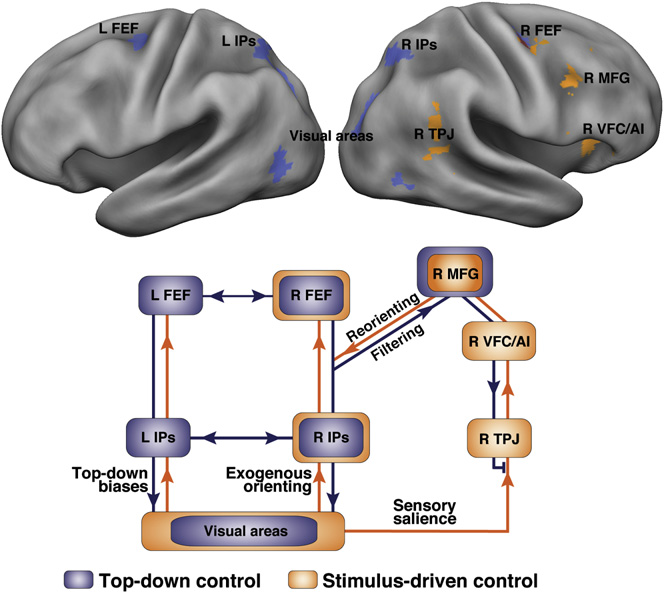
\includegraphics[scale=0.4]{img/attentionnetworks.png}
	\caption[Dorsal and ventral attention networks]
	{\small{Definition of dorsal and ventral networks from activation data and putative interactions. Taken from Corbetta, Patel \& Shulman, 2008.}}
	\label{fig:Networks}
\end{figure}

\subsection{The frontal eye fields}
A core part of the dorsal attention system are the FEF. In humans, the FEF is located in the rostral bank of a portion of the precentral sulcus at the caudal end of the middle frontal gyrus. It is primarily involved with transforming sensory signal into motor commands for intentional conjugate visual exploration to the contralateral visual space, and it is active in the disengagement from fixation that must precede each refixation saccade (Goodwin, 2007; Tehovnik et al., 2000). Early insights about its function stem from stimulation studies with primates. Low-intensity electrical stimulation of the FEF in the bank of the arcuate sulcus in monkeys elicits saccadic eye movements directed contralateral to the stimulated hemisphere (Tehovnik et al., 2000; Schall, 2009). Early work by Bruce and colleagues (1985) found that saccades elicited by stimulation at a particular region have a particular direction and amplitude that is independent of the orientation of the eyes. It further revealed a gradient of saccadic amplitudes from lateral to medial sites of the FEF: The more medially the stimulation of the primate arcuate sulcus, the larger the saccadic amplitude (Bruce et al., 1985). Hence, the ventrolateral portion of the FEF is generating shorter saccades, while the mediodorsal portion is generating longer saccades. Stimulation studies in primates and high resolution fMRI experiments in humans further revealed that while the FEF is best known for its role in the generation of rapid saccadic gaze shifts, it also contains zones that are involved in the  control of other types of eye movements, among them pursuit, fixation, and vergence (changes of the depth of the gaze) eye movements (Krauzlis, 2013): Stimulation of the frontal pursuitzone in the fundus elicits pursuit eye movements directed ipsilateral to the stimulated hemisphere (Schall, 2009). The intracortical stimulation of several subareas within the FEF, among others a region within the pre-arcuate cortex in rhesus monkeys, immediately rostral to the saccade related anterior bank of the arcuate sulcus, triggers vergence movements, and shows the areas involvement in accomodation and the sensorimotor transformations required for these movements (Crosby et al., 1952, cited by Vernet, Quentin, Chanes, Mitsumasu \& Valero-Cabre, 2014). The FEF, therefore, seems to play a crucial role in all kinds of eye movements. \newline
However, as its involvement in the dorsal attention network suggests, the FEF is further involved in a number of aspects of higher cognition, such as visuospatial attention, visual awareness, and perceptual modulation.  In a human rTMS study, Muggleton and colleagues (2003) found rTMS at 10Hz for 500ms over the right FEF impaired only those subtypes of visual search where a visual target is neither salient nor predictable, and hence involving endogenous visuospatial attention. More evidence for the involvement of the FEF in higher cognitive functions necessary for target selection was found in primates (Thompson \& Bichot, 2005). \newline
As such, the involvement of the FEF in the various types of eye movements is modulated by the cognitive context (Vernet, Quentin, Chanes, Mitsumasu \& Valero-Cabre, 2014).
The connectivity of the FEF with visual areas caudal to the central sulcus is topographically organized. The more ventrolateral portion of the FEF, which is responsible for generating shorter saccades, is interconnected with the perifoveal representation in retinotopically organized areas, from areas that represent central vision in the inferotemporal cortex and from other areas having no retinotopic order. In contrast, the mediodorsal FEF, which is responsible for generating longer saccades, is interconnected with the peripheral visual field representation of retinotopically organized areas, from areas that emphasize peripheral vision or are multimodal and from other areas that have no retinotopic order (Schall, 2009).


\section{Movements of the eye}
A central feature of the human retina is the fovea centralis, a specialised region about 1.5mm in diameter in the center of the retina (Benninghoff \& Drenckhahn, 2004). It serves only the central 1$^\circ$ of the visual field, but due to possessing the highest amount of cones of the retina, and an asymmetric distribution of ganglion cell density across the retina that advantages foveal information, it provides the greatest visual acuity (Perry \& Cowey, 1985). This asymmetry is propagated in the cortical representation of visual inputs from the retina. The magnification factor (MF), the linear extent of cortex devoted to each linear degree on the retina (Daniel \& Whitteridge, 1961), increases monotonically from periphal to foveal vision (Daniel \& Whitterage, 1961). As a result, in almost all visual brain areas, both cortically and subcortically, the fovea has the greatest representation. Full visual acuity can therefore only occur at the fovea. 
Due to this constraint, humans need the ability to, first, align the fovea rapidly to an object of interest and, second, keep the fovea aligned to it for a sufficient amount of time in order to maximize the efficiency of foveal vision and perceive objects of interest in greatest detail. An exploration of a visual scene is hence performed in a stepwise manner and requires the described sequence of eye movements to sequentially explore all areas of interest. To accomplish this, the human eye is capable of a number of different eye movements. A selection of important eye movements will be introduced briefly in this section. \newline
In its most simple form, the sequence consists of rapid eye-movements, so called \textit{saccades}, redirecting the fovea from one object of interest to the next, followed by phases of \textit{fixation} that keep the fovea aligned for visual analysis. As saccades reach speeds of up to 500 $^\circ$/sec, small, corrective post-saccadic oscillations, so called \textit{glissades}, correct minor deviations of saccade target and actual saccade endpoint. Additionally, \textit{smooth pursuits} enable a viewer to track moving objects, while \textit{vergence} movements are necessary for accommodating different depths (Holmqvist \& Nyström, 2011). The following table \ref{table:eyemovements} provides an overview of these movements and their characteristics. 
  
\begin{table}[H]
	\begin{center}
		\begin{tabular}{lC{3cm}C{3cm}C{3cm}}
			\thickhline 
			\textbf{Type}	& \textbf{Duration(ms)} & \textbf{Amplitude (degrees)} & \textbf{Velocity ($^\circ$/sec)} \\ \hline
			Fixation 		& 200-300  & -  &  - \\
			Saccade 		& 30-80   & 4-20  & 30-500 \\
			Glissade			& 10-40   & 0.5-2  & 20-140 \\
			Smooth pursuit			& -  & -  &  10-30 \\ \thickhline
		\end{tabular}
		\caption[Movements of the eye]{\small{An overview of major types of eye movements and their characteristics, taken from Holmqvist \& Nyström (2011).}}
		\label{table:eyemovements}
	\end{center}
\end{table}

Note, however, that most work on eye movements was conducted on static stimuli, and eye movements on moving images could possess differential characteristics. Dorr, Martinez, Gegenfurtner and Barth (2010) for example investigated fixation characteristics differentially for varying stimuli and found Hollywood movies to elicit longer fixations (mean: 354ms, median: 253ms) than static images. \newline
Saccadic eye movements are controlled by a number of highly interconnected brain regions, among them cortical structures in frontal and parietal areas such as the frontal and supplementary eye field (FEF, SEF) and lateral intraparietal area (LIP), as well as subcortical structures such as the basal ganglia, thalamus, cerebellum, reticular formation, and superior colliculus (Munoz, 2002, see figure \ref{saccregions}). In the cortex, the frontal eye fields (FEF) are seen as the principal region involved in oculomotor control (Leichtnetz \& Goldberg, 1988).

\begin{figure}
	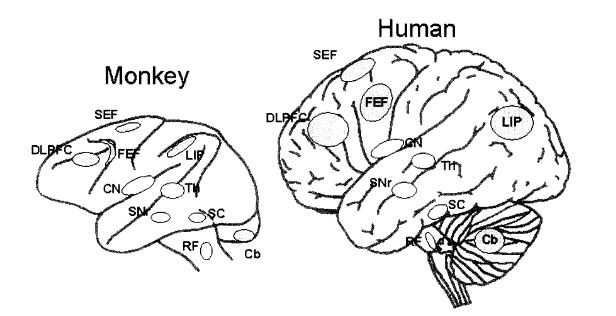
\includegraphics[scale=0.5]{img/saccregions.png}
	\caption[Regions involved in saccadic eye movements]{\small{Brain areas involved in the control of saccadic eye movements in monkey (left) and human. \textit{Cb}: Cerebellum, CN: Caudate nucleus, \textit{DLPFC}: dorsolateral prefrontal cortex, \textit{FEF}: Frontal eye field, \textit{LIP}: Lateral intraparietal area; \textit{RF}: Reticular formation, \textit{SC}: superior colliculus, \textit{SEF}: supplementary eye field, \textit{Snr}: substantia nigra pars reticularis, \textit{Th}: Thalamus. (Taken from Munoz, 2002)}}
\end{figure}

\section{title}

\section{Insights on function and location from naturalistic stimulation}
Visuospatial attention is usually studied by means of highly controlled experimental tasks, such as Posner’s (1980) cueing paradigm or simple visual search tasks. While well controllable, these conventional laboratory experiments suffer from a lack of ecological validity and fail to evoke realistic competing demands for visuospatial attention. As Hasson and colleagues (2004) noted, controlled experimental settings bear little resemblance to natural viewing for at least four reasons: 1) Lack of complex visual scenes (i.e. presentation of visual stimuli in isolation), 2) Lack of (complex) movement, 3) Lack of unconstrained eye movement, and 4) Lack of interactions between vision and additional modalities, context and emotional valence. Naturalistic stimulation such as watching movie clips, in contrast, does not suffer from these shortcomings and, as Hasson, Malach and Heeger (2010) showed, does also not lack experimental control. During the past decade, therefore, while static images have been an object of interest in the analysis of gaze distribution and attention from the early works of Yarbus (1967) onwards, movies or videos became a promising stimulus choice as well. They contain interesting, multisensory stimuli and are more representative of natural vision arrays than static pictures. As movie content constantly changes and includes both salient elements such as motion, as well as top-down components from the attempts to comprehend and interpret the content (Ross \& Kowler, 2011), movies represent an ideal possibility to study the dynamic and complex interplay of attention networks ecologically valid   (e.g. in Hasson, Nir, Levy, Furhmann \& Malach, 2004; Carmi \& Itti, 2006; Tseng, Carmi, Cameron, Munoz \& Itti, 2009; Dorr, Martinetz, Gegenfurtner \& Barth, 2010). \newline
Localization of areas such as the FEF in turn is most reliably conducted via micro-stimulation in animals. Localization through non-invasive methods in humans is more challenging, but studies employing positron emission tomography (PET) (e.g. Paus, 1996, Kawashima et al., 1998), magneto-encephalography (MEG) (e.g. Ioannides et al., 2004), fMRI (e.g. Petit \& Haxby; Connolly, Goodale, Menon \& Munoz, 2002), and transcranial magnetic stimulation (TMS) (see Vernet et al., 2014, for an overview) were able to shed light on the possible location of the FEF in humans.  However, an overall view of this literature also reveals the large variability of reported localizations between studies (see e.g. Paus, 1996; Vernet et al. 2014, for overviews). The methods for FEF localization usually are behavioral paradigms with either general oculomotor tasks (Paus, 1996), or more specific oculomotor task such as instructed fixations, pro- and antisaccades (Connolly et al., 2002) or tracking of horizontal step stimuli (Alkan, Biswal \& Alvarez, 2011). While capable of localization, the resulting movements are not performed under unconstrained conditions and it remains unknown whether uncontrolled eye movements under naturalistic viewing behavior can be capable of providing similar location information as well, if not even additional information when taking cognitive context such as attention deployment into account.\newline
Therefore [ELABORATE ON WHY FEF ARE IDEAL TO STUDY UTILIZATION OF EYEMOVEMENTS; VISUOSPATIAL ATTENTION (shedding more light on the role of the FEF under differential attentional modes), LOCALIZATION]
The thesis at hand therefore has the following objectives:
- Investigate a plausible method to utilize eye movements for the analysis of fMRI data with regard to visuospatial attention
- Derive, implement, and test a novel method of localization
- Combine both subgoals for a localization of the FEF with eye gaze and attention measures

Due to its ready availability coming from the Psychoinformatics Lab itself, its incredible data richness, and its employment of naturalistic stimuli in form of a Hollywood movie, the studyforrest datasets were selected as the data basis of the analysis.

\section{Utilizing eye movements in the study of attentional deployment}
[Something about overt and covert attention here]
[something about attentional focus following eyegaze here]
[now bridge to scanpaths]
\subsection{Scanpaths}
The term scanpath refers to the trace of eye-movements in space and time (Holmqvist \& Nyström, 2011). In its most simple form, it is formed by a succession of fixations and saccades that define the particular sequence in which the eyes explore a visual scene (Anderson, Anderson, Kingstone \& Bischof, 2015). As opposed to other measures that summarize eye gaze, such as heatmaps, and as  emphasized by Nytröm \& Holmqvist (2011), the order of eye-movements is relevant - a different order of elements in the representational sequence of eye-movements constitutes a different scanpath. \newline
The analysis of scanpaths has been used for decades to gain insights into the viewers’ mental processes, especially those concerning visuo-spatial attention. Yarbus (1967) wrote: 

\begin{quotation}
\footnotesize{„Eye-movements reflect the human thought processes; so the observer‘s thoughts may be followed to some extent from records of eye-movements (the thought accompanying the examination of the particular object). It is easy to determine from these records which elements attract the observer‘s eye (and, consequently, his thought), in what order, and how often“.}
\end{quotation}

Following this reasoning, the comparison of scanpaths of different subjects constitutes a measure of similarity in the different subjects’ attentional processes and adds a useful dimension to the traditional analysis of eye-tracking data. In recent years, many approaches for scanpath comparisons were developed and implemented in various software solutions. Among them are methods based on (semantic) areas of interest (AOIs) such as the \textit{Levenshtein distance} (Levenshtein, 1966), or an improved generalization of it in \textit{ScanMatch} (Christino, Mathot, Theeuwes \& Gilchrist, 2010), methods based on attention maps such as \textit{AMAP} (Ouerhani, von Wartburg, Hugli \& Muri, 2004), methods employing machine learning algorithms such as \textit{SMAC with HMM} (Coutrot, Hslao \& Chan, 2018), or methods based on vector-geometry such as \textit{MultiMatch} (Jarodzka, Holmqvist \& Nyström, 2010). The latter method has been developed specifically to overcome known shortcomings of many previous methods that limit their informative value, stemming from a loss of information due to the use of coarse aggregate measures of eye movement, susceptibility of the results of a comparison to influential data points due to arbitrary classifications, or both. The method does not rely on AOIs and hence achieves a finer level of detail in scanpath comparison. It takes temporal order, location in space, durations of fixations, and the shape of eye-movements into account, and is thus a comprehensive evaluation of multiple scanpath characteristics. In evaluations with simulated and actual eye-tracking data, the method was found to be robust against spatial noise, sensitive to position, order and fixation duration, and outperformed the ScanMatch method in AOI border cases (Dewhurst et al., 2012). In a comprehensive test of eleven common scanpath comparison methods on static real-life photographies, MultiMatch was found to be robust in general, however with high differences in the duration measure depending on the viewing time for the stimuli (Anderson, Anderson, Kingstone \& Bischof, 2015). As it additionally was successfully used to study mental activity involved in perceiving visual input by others (French, Glady \& Thibaut, 2017) already, the MultiMatch method was chosen to be employed in the current thesis to derive a measure for attentional processes of participants during movie watching. 
The original implementation, however, only existed as a Matlab toolbox shared upon request by the corresponding author of the respective publication (Dewhurst et al., 2012). This reliance on closed-source software and barriers in retrieval of the software\footnote{While acquisition of the toolbox via e-mail was prompt and complication-free, later correspondence with several of the authors was an odyssey of expired email addresses, changed affiliations and digital communication allegedly lost in the void of the Internet.} hinder the wider usage and potential improvement of the method. A publicly available, open-source implementation however would instead facilitate scientific work. Therefore, the method was ported from Matlab into Python and transformed into the pip-installable module multimatch\footnote{The module can be install via ```pip install multimatch```. A corresponding publication (Wagner \& Hanke) in the Journal of Open Source Software (JOSS) in currently under review. The sourcecode can be found at github.com/AdinaWagner/multimatch}.

\section{Localization based on sensitivities weights}
Something about the main idea behind this approach here

\subsection{Classification Analysis in Machine Learning}
Machine learning refers to the study and construction of software that can learn from data without being explicitly programmed. Especially in the data-rich environment of neuroimaging, machine learning algorithms and techniques have gained immensely in popularity and significance as for their ability to detect hidden patterns and trends in the data (Vogt, 2018). For clarity, two sets of terms used in machine learning are defined at this point.
The terms “variable”, “feature”, “attribute” or “dimension” are used interchangeably to refer to different information pieces about the sample and can be thought of as the columns of a dataset. In the given thesis, each timepoint of a brainscan is a feature. The terms “sample” or “instance” on the other hand are used interchangeably to refer to different data entities and can be thought of as the rows of a dataset. In this thesis, one sample may be the activation of a voxel. For every feature (timepoint) the sample (voxel) will display a particular activation.
The general approach for implementing machine learning systems is to train a model on a subset of data (the training set) and test the model on a previously unseen subset of data (the test set) to see how well it generalizes from what it learned. A machine learning model is subsequently evaluated based on its performance on the training and the test set (Nguyen \& Zeigermann, 2018). 
One particular category of machine learning techniques is classification. In classification, the goal of an analyses is to predict a category of an outcome. An easily comprehensible example may be predicting the weather (sunny, cloudy, rainy) on different days (samples) based on different weather features (air pressure, wind speed, humidity, temperature). One famous historic example of such classification problems is the identification of hand-written digits in the postal system to make zip codes machine readable (Le Cun, Boser, Denker, Handerson, Howard, Hubbard \& Jackel, 1990).  In brain imaging in turn, an example may be the classification of voxels to functional regions (Nastase, Guntupalli, Haxby \& Halchenko, 2016). 
Classification is generally a supervised machine learning problem. In supervised ML, the classification model, often termed classifier, is trained on a subset of data in which the target (= the outcome the model is predicting) is provided, i.e. the data is „labeled“. The successive test dataset the classifier is applied to is unlabeled.



\chapter{Methods}\label{par:methods}

The following method section attempts to give a concise description of this thesis' data basis, fMRI and eye-tracking, and the employed and developed methods, MultiMatch and sensitivity analysis. 

\section{Data basis}

Data stems from the 2016 released extension of the studyforrest dataset (Hanke et al., 2016; Sengupta et al., 2016; all data and code publicly available at https://github.com/psycho-informatics-de/studyforrest-data-phase2). In this extension, $N = 15$ right-handed participants (age range 21 – 39 years, mean age 29.4 years, six female, normal or corrected-to-normal vision), who had previously participated in the studyforrest project, watched the audio-visual movie “Forrest Gump” (R. Zemeckis, Paramount Pictures, 1994) during simultaneous fMRI and eye-tracking recording, and underwent a traditional localizer paradigm for higher visual areas: The fusiform face area (FFA), the occipital face area (OFA), the extrastriate body area (EBA), the hippocampal place area (PPA), the lateral occipital complex (LOC) and early visual cortex (Sengupta et al., 2016).

\subsection{Stimulus material}

Stimulus material for the audiovisual movie was the German dubbed version of Forrest Gump, overlaid with a German audio-description (Koop, Michalski, Beckmann, Meinhardt \& Benecke, produced by Bayrischer Rundfunk, 2009), originally broadcast as an additional audio track for visually impaired recipients on Swiss public television. The additional audio track consists of a male narrator describing the visual content of a scene between dialogs, off-screen-speech or any other relevant audio-content of the movie (Hanke et al., 2014). The video track for the movie stimulus was re-encoded from Blu-ray into H.264 video (1280 x 720 at 25 frames per second (fps)). In accordance to the procedure in an earlier phase of the studyforrest project, the movie was shortened by removing a few scenes less relevant for the major plot to keep the fMRI recording session under two hours. The shortened movie was then segmented into eight segments of roughly the 15 minutes of length (for an overview on segment duration, final stimulus content and detailed procedures see Hanke et al., 2014). Stimulus material for the localizer paradigm consisted of 24 unique grayscale images for each of six different categories (faces, bodies, houses, scenes, everyday objects, and scrambled images) at a resolution of 400x400px, matched in luminance, and displayed at 10x10$^\circ$ of visual angle (Sengupta et al., 2016).

\subsection{Procedures}
Functional MRI data acquisition for the audio visual movie was undertaken in two consecutive recording sessions on the same day, with a break of flexible duration. Within each session, four movie segments were presented in chronological order (Hanke et al., 2016).  Prior to each segment an eye-tracker calibration with a 13-point sequence and accuracy validation was performed.
Segments were succeeded by another accuracy validation and participants were asked to rate their experience (“How deeply did you get into the story?”) on a scale from 1 (not at all) to 4 (a lot). Visual stimuli were projected on to a screen inside the bore of the magnet using an LCD projector, and presented to the subjects thought a front-reflective mirror on top of the head
coil at a viewing distance of 63cm. The screen dimensions were 26.5cm x 21.2cm at a resolution of 1280 x 1024 px with a 60Hz video refresh rate (Sengupta et al., 2016). Eye-tracking was performed with an Eyelink 1000 (software version 4.594) using monocular corneal reflection and pupil tracking with a temporal resolution of eye gaze recordings of 1000Hz. The camera was mounted at an approximate distance of 100cm to the left eye of subjects, which was illuminated
by an infrared light source (Hanke et al., 2016). Movie presentation and eye-tracking were synchronized by starting the eye gaze recording as soon as the stimulus computer received the first fMRI trigger signal. Timings of subsequent trigger pulses and onsets of every movie frame
were logged. Using a 3 Tesla Philips Achieve dStream MRI scanner with a 32 channel head coil, T2*-weighted echo-planar images (gradient-echo, TR = 2s, echo time = 30ms, flip angle = 90) were acquired during movie watching. For the eight segments, 451, 441, 438, 488, 462, 439, 542, and 338 volumes were acquired, respectively (Hanke et al., 2016).

In the localizer paradigm, participants viewed the different object categories in a total of four block-design runs, with two 16s blocks per stimulus category. The order of the individual images per category differed across runs and participants, but the sequence of category blocks was the same for every run and participant. Localizers for higher visual areas (FFA, OFA, PPA, LOC, EBA, and early visual cortex) were obtained by the original authers of the studyforrest extension by means of the two-level GLM analysis on contrasts of activation between objectcategories (for details, see Sengupta et al., 2016).

\subsection{Preprocessing of eye-tracking data}
Eye-tracking data were normalized such that all gaze coordinates are in native movie frame pixels, with the top-left corner of the movie frame located at (0, 0) and the lower-right corner located at (1280, 546) (Hanke et al., 2016). The amount of unusable data, primarily due to signal loss due to eye blinks, ranged from less than 1 to 15\% for 13 of the 15 in-scanner subjects (the other two subjects’ data contained 85 and 36\% of data loss, respectively). More contiguous data was yielded in the laboratory acquisition. In-scanner acquisition had an approximate spatial uncertainty of 40px according to the calibration procedure. \newline
The raw eye tracking data was classified into different eye movements. For this, based on an adaptive, velocity-based algorithm proposed by Nyström and Holmqvist (2010), Dar, Wagner and  Hanke (in preparation) implemented a data-driven algorithm for robust eye movement detection for natural viewing (REMoDNaV) in Python, independent of this thesis\footnote{The sourcecode can be found at github.com/psychoinformatics-de/remodnav}. All results of this algorithm are publicly available at [URL here]. The algorithm categorizes the raw data into the eye movement categories saccades, fixations, post-saccadic oscillations (glissades), and disregards any unclassifiable data (such as blinks). The eye events are reported together with their start- and end coordinates, their onsets and duration in seconds, their velocity and the average pupil size.

\subsection{Extraction and processing of eye tracking data}

For the extraction of saccadic eye events, the results where filtered to include only saccades. For the computation of event files following the BIDS standard (Gorgolewski et al., 2016), the Cartesian coordinates of the saccades were transformed into Polar coordinates (angle and length). Based on their angle, saccades were classed into event types describing eight different orientations in the visual field. Saccade onsets and durations were extracted from the REMoDNaV output. The resulting event file per run hence contained the onset, duration, amplitude (length) and direction of saccades. \newline


\section{MultiMatch}
For the purpose of this thesis, the MultiMatch method for scanpath comparison (Jarodzka, Holmqvist \& Nyström, 2010) was ported into Python for further use on the preprocessed eye movement data. An overview in pseudocode is outlined in algorithm \ref{algo:multimatch}. \newline 
The method takes two n x 3 fixation vectors of two scanpaths with x-coordinates, y-coordinates, and duration of fixations as columns as its input. Based on the coordinates and durations of fixations, the scanpaths are represented as geometric vector sequences as shown in figure \ref{fig:Polar_to_cartesian}:

\begin{figure}[H]
		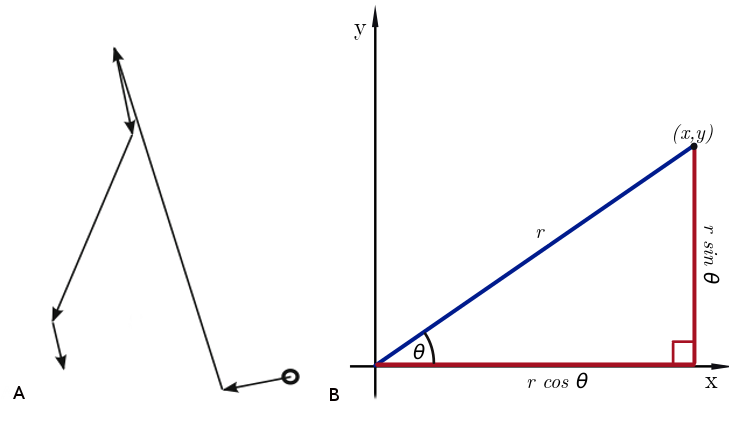
\includegraphics[scale=0.35]{img/scanpathconversion.png}
		\caption[Geometric representation of eye movements]
		{\small{\textit{A: Geometric scanpath representation.} An idealized saccade is represented as the shortest distance between two fixations. The Cartesian coordinates (x, y) of the fixations are thus the starting and ending points of a saccade. The length of a saccade in x (or y) direction is computed as the difference in x (or y) coordinates of starting and ending point. \newline
		\textit{B: Length and angle computation.} Length from the coordinate origin, rho, is computed as the Euclidean norm by means of the Pythagorean theorem: $r = \sqrt{ x^2 + y^2}$. The angle in radians, theta, is computed as a variation of the arctangent function as the angle from positive x axis to the point (x, y), with positive values denoting counterclockwise angle from positive x axis and negative values denoting clockwise angles: $\theta = arctan2(x, y)$.}}
		\label{fig:Polar_to_cartesian}
\end{figure}

To reduce complexity, the scanpaths are simplified according to angle and amplitude (length) in an iterative procedure. Two or more saccades are grouped together if angles between two consecutive saccades are below an angular threshold \textit{TDir}, or if the amplitude of successive saccades is below a length threshold \textit{TAmp}, as long as intermediate fixations of the saccades are shorter than a duration threshold, \textit{TDur}. As such, small, locally contained saccades, and saccades in the same general direction are summed to form larger, less complex saccades. \newline
In order to find pairings of saccade vectors to compare, the simplified scanpaths are temporally aligned. The aim is to not necessarily align two saccade vectors that constitute the same component in  their respective vector sequence, but those two vectors that are the most similar while still preserving temporal order. In this way, a stray saccade in one of the two scanpaths does not lead to an overall low similarity rating, and it is further possible to compare scanpaths of unequal length.  To do so, all possible pairings of saccades are evaluated in similarity by the vector differences between all pairings (shape: The vector differences between each element $i$ in scanpath $S1 = {u_1, u_2, \ldots, u_m}$ and each element $j$ in scanpath $S2 = {v_1, v_2, \ldots, v_n}$ are computed an stored in a Matrix $M$ as weights that denote similarity, with low weights corresponding to high similarity. In a next step, an adjacency matrix is build, defining the rules on which connection between matrix elements are allowed to preserve the temporal order of saccades. Together, matrices M and the adjacency matrix constitute a matrix representation of a directed, weighted graph (\ref{fig:directedgraph}). Elements of the matrix are nodes, the connection rules constitute edges and the weights define the cost associated with each connection. 
In the generic example in figure \ref{fig:directedgraph} the edge between node (1, 1) and node (1, 2) has an associated weight, or cost, of $w_2$. 


\begin{figure}
	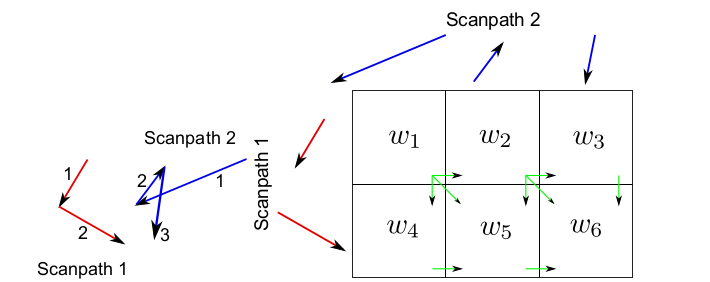
\includegraphics[scale=0.4]{img/weightedgraph.png}
	\caption[Scanpath alignment as a shortest-path-problem]
	{\small{The elements of two hypothetical scanpaths (left) are used to compute vector differences between all possible pairings as weights $w_1, \ldots, w_6$ in a Matrix $M$ (right). Green arrows indicate connection rules defined by an adjacency matrix. Taken from Jarodzka, Holmqvist \& Nyström, 2010.}}
	\label{fig:directedgraph}
\end{figure}

A Dijkstra algorithm (Dijksta, 1959) is used to find the shortest path from the top left node, the first two saccade vectors, to the bottom right node, the last two saccade vectors. “Shortest” path is defined as the connection between nodes with the lowest possible sum of weights. The path returned by the Dijkstra algorithm is a sequence of indexes, denoting pairings of saccade vectors from each scanpath, and as such the desired alignment of scanpaths (Dewhurst et al., 2012).  Finally, in a last step, five measures of scanpath similarity (see figure \ref{fig:simmeasures}) are computed for a multidimensional similarity evaluation. This is done by performing simple vector arithmetic on all aligned saccade pairs $(u_i, v_j)$, normalizing the results according to a certain metric, and taking the median of the results. All five measures are in range [0; 1] with higher values indicating higher similarity between scanpaths on the given dimension. \newline

\begin{figure}
	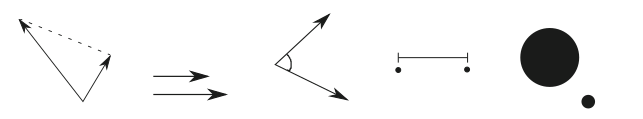
\includegraphics[scale=0.5]{img/simmeasures.png}
	\caption[Similarity measures]{\small{\textbf{Shape}: Vector difference between aligned scanpaths, normalised by 2x the screen diagonal. \textbf{Length}: Difference in vector lengths, normalized by the screen diagonal. \textbf{Angle}: Angular distance between saccade vectors, normalized by $\pi$. \textbf{Position}: Position difference of fixation, normalized by the screen diagonal. \textbf{Duration}: Duration differences of aligned fixations, normalized against maximum duration within the comparison.}}
	\label{fig:simmeasures}
\end{figure}


\begin{algorithm}
	\SetKwInOut{Input}{Input}
	\SetKwInOut{Output}{Output}
	
	\Input{nx3 fixation vectors (x, y, duration), simplification thresholds $T_{Amp}$, $T_{Dir}$, $T_{Dur}$}
	\Output{eventfile: onset of scanpath, duration, and five similarity measures range [0;1]}
	\For{each fixvector}
	{ 
		\For{fix in fixvector}
		{
			fixation\_x, fixation\_y, fixation\_dur = $x, y, duration$ \;
			saccade\_x(y) = fixation\_x(y)$_{fix}$ $-$ fixation\_x(y)$_{fix+1}$ \;
			saccade\_lenx(leny) = fixation\_x(y) $-$ saccade\_x(y)\;
			saccade\_rho, saccade\_theta = cartesian2polar(saccade\_lenx, saccade\_leny) \;
			\textbf{eyedata} = [fixation\_x, fixation\_y, fixation\_dur, saccade\_x, saccade\_y, \newline saccade\_lenx, saccade\_leny, saccade\_rho, saccade\_theta]
		}
		\While{simplification is still possible}{
			\If{angle(saccade$_{i}$, saccade$_{i+1}) < TDir$ \bfseries{and} $fixation\_dur < TDur$}
			{combine saccades}
			\If{saccade\_rho$_i$, saccade\_rho$_{i+1}$) < TAmp \textbf{and} fixation\_dur $<$ TDur}{combine saccades}
		}
		\For{pair of (simplified) scanpaths $S1 = \{u_1, \ldots, u_m\}, S2 = \{v_1, \ldots, v_n\}$}
		{
			calculate M: Matrix of saccadelength differences between each $i \in S1$ and  $j \in S2$\;
			create a directed graph with elements of M as weights $w_1, \ldots, w_i$\;
			align scanpaths with $min(\sum w)$ from $M(0,0)$ to $M(n,m)$ via Dijkstra algorithm\;
		}
		\For{pair($u_i,v_i$) in aligned scanpaths}
		{
			angular difference = angle($u_i, v_1$)\;
			position difference = $\sqrt{(x(u_i) - x(v_i))^2 + (y(u_i) - y(v_i))^2}$ \;
			vector difference = $\sqrt{(len\_x(u_i) - len\_x(v_i))^2 + (len\_y(u_i) - len\_y(v_i))^2}$\;
			length difference = $abs(rho(u_i) - rho(v_i))$\;
			duration difference = $abs(dur(u_i)-dur(v_i))$ \;
		}
		normalize angular difference by $\pi$\;
		normalize vector difference by 2x the screen diagonal (maximum theoretical distance)\;
		normalize length difference by the screen diagonal\;
		normalize position difference by the screen diagonal\;
		normalize duration difference by maximal duration difference in the scanpaths\;
		\textbf{return} median for each similarity measure
	}
	return \textbf{similarity measures}
	\caption{The MultiMatch Algorithm}
	\label{algo:multimatch}
\end{algorithm}

\subsection{MultiMatch and the studyforrest dataset: multimatch\_forrest}
The extraction and processing of eye events for further use with multimatch to estimate a measure of exogenous attentional control included several considerations based on findings and known caveats in eye tracking and attention research with dynamic scenes. These considerations were implemented as additional functionality of the multimatch module to natively work with the studyforrest dataset as a data basis in the function \textit{multimatch\_forrest}. The additional functions are distributed along with the main algorithm in the multimatch module and are mainly concerned with automatic scanpath extraction from the approximately 15 minutes spanning and several eye-movement categories containing eye-tracking event files by user-defined rules. An overview in pseudocode can be found in algorithm \ref{algo:multimatch_forrest}. \newline
First, as the stimulus was dynamic, the start and end of pursuit movements were relabeled as fixations. This was done to accomodate the fact that most areas of interest in a movie are in motion, and what would be a fixation while viewing a static image would likely be a slow pursuit during movie watching. A different consideration concerned the selection of scanpaths from the ~15 minute segments, as their length is unsuitably long to derive a continuous attention measure or do a scanpath comparison on. It has been shown that subjects gazes have a bias towards the center in Hollywood movies (Tseng, Carmi, Cameron, Munoz \& Itti, 2009). This bias can at least in part be traced back to a strong center bias directly after cuts in dynamic scenes. Carmi and Itti (2006) found the highest degree of exogenous attentional control (i.e. maximal inter-observer similarity in gaze as recorded via eye-tracking) in a moving collage of 50 heterogeneous video clips directly after cuts to new, semantically unrelated scenes. Without isolating cuts it therefore can not be disentangled whether the contribution of visual features of the movie on scanpaths stems from exogenous control from a movie element or from the sudden occurrence of a new scene after a cut. To not introduce such a confound in the eye-tracking data, the data was cut into shots that did not contain cuts to different scenes, relying on a location annotation by Häusler and Hanke (2016). The location annotation contained a detailed description of the timing of each of the 870 shots of the movie as well as information about the depicted location in different levels of abstraction. A shot is defined as a movie sequence between two cuts. In a first step, all consecutive short shots to the same locale (e.g. two consecutive, short movie shots in Forrest's bedroom, without any cuts containing semantically unrelated content) were grouped together. A “short” shot was defined as being shorter than the median length of 4.92s. This increased the median length of shots from 4.92s to 7.019s. These elongated shots are henceforth referred to as snippets. In a next step, within the scanpath comparison, the onset and offset times of the resulting snippets were extracted for every snippet longer than 4.92s. To not introduce an influence of snippet length into the similarity results, as longer movie snippets will be more likely to be less similar than short ones, scanpath lengths were standardized to approximately 4.92s seconds (the original median length). To further evade any problems associated with the center bias, scanpaths were extracted from the end of the snippet: The last oculomotor event within the range of the snippet marked the end of a scanpath. As such, scanpaths began maximally distant to the snippet onset.
As the eye movements of participants are interindividually different and don't correspond exactly to snippet timing, the precise onsets and resulting exact durations were computed as well, and stored for later use as regressors.

\begin{algorithm}
	\SetKwInOut{Input}{Input}
	\SetKwInOut{Output}{Output}
	
	\Input{REMoDNaV eye movement datafiles per run, movie location annotation per run, desired length to elongate shots to \textit{ldur}, desired scanpath length \textit{dur}}
	\Output{One n x 3 fixation vector (x, y, duration) per shot > dur}
	{
		\If{$event_{row}$ == pursuit}
		{
			regard start and end points of pursuit as fixation
		}
	}
	\For{row in REMoDNaV datafile}
	{
		\If{$event_{row}$ == fixation}{
			extract x-, y-coordinate, duration}
		\If{x, y < 0 or x > 1280 or y < 720}{discard as out-of-bound gaze}
	}
	\For{row in annotation}
	{
		\If{($locale_{row} == locale_{row+1}$) and ($duration_{row}, duration_{row+1} < ldur$)}
		{combine to one shot}
	}
	\For{row in annotation}
	{
		\If{$duration_{row}$ > dur)}
		{extract shotonset and offset time}
	}
	\For{i in length(onset)}
	{fixvector$_i$ = REMoDNaV[REMoDNaV$_{onset} > onset_i$; REMoDNaV$_{onset}$ < offset$_i$]
	}
	return $\{$fixvector$_1$, \ldots, fixvector$_i$$\}$, onsets, durations
	\caption{The studyforrest specific functions of multimatch}
	\label{algo:multimatch_forrest}
\end{algorithm}






\chapter{Results}

\subsection{Eye movements}
In order to check the validity of the eye-movement extraction with REMoDNaV, the mean and median duration of extracted fixations were compared to the results of Gegenfurtner et al. (2010). Fixations as found by REMoDNaV had a length of mean = 0.326s, median = 0.256s, which corresponds closely to the aforementioned study's results (0.354s and 0.253s, respectively). Moreover, a comparison of algorithm performance and human coding in the spirit of Anderson et al. (2017) by Dar, Wagner and Hanke (in preparation) showed the highest degree of concordance of all contemporary algorithms used in Anderson et al. (2010).

\bigskip





\section{Gunnar}

Macro stress testing is an incremental part of managing a bank's risk and assessing the vulnerability of financial institutions to macroeconomic shocks. 
It examines the impact of adverse scenarios on the bank's capital. 
The results should provide the relevant stakeholders and the public with information on the bank's resilience. The main issue is the ability of institutions to cushion shocks and meet capital requirements in an unfavourable financial environment.
The influence of the macroeconomic conditions on the default behaviour of retail and corporate customers in a bank's portfolio is of recent interest for financial institutes as well as for research. In this context, stress testing is a well-established tool of the risk management and banking supervisory institutions to quantify the aggregated impacts of severe but plausible macroeconomic downturn scenarios on a bank's risk exposure.
For this purpose, the probability of default of customers is a key factor for the credit risk assessment in the financial services business.

This master thesis has the objective to develop and compare so called \textit{satellite models} \linebreak for macro stress testing with application to the Volkswagen Bank GmbH's credit portfolio. By satellite models we understand modelling techniques that establish a link between certain macroeconomic drivers and aggregated bank-specific risk parameters. It denotes a risk model that is used to translate a given macroeconomic scenario into risk parameters at the firm level.
The credit risk satellite model is of crucial importance in the stress testing context, since this risk category is the most material risk in the Volkswagen Bank GmbH.

\bigskip

In the course of this thesis, it is examined which models are suited to establish a relationship between the macroeconomic development and the bank-specific default rates on an aggregated portfolio level. We use the average default rate as a proxy for the underlying probability of default.
The challenge for this study is in particular the poor data basis. The time series of historical default rates are relatively short and contain to some extent structural breaks. Therefore, solution strategies on how to address these issues are discussed. Based on appropriate model selection criteria it will be investigated which model is suited best for the application in the Volkswagen Bank GmbH.
Methodologically, the available internal historical time series of average country-specific default rates in the retail and the corporate dealer portfolios, respectively, are explained by models in dependence on macroeconomic variables such as the gross domestic product, the unemployment rate, the automobile sales volume and interest rates.
The functional link is then used for the purpose of stress testing to predict the impact of macroeconomic downturn scenarios on the default rates. 

\pagebreak

This master thesis is structured as follows. Chapter \ref{par:stresstesting} introduces the topic of stress testing and gives an overview of the pertinent literature. In chapter \ref{par:data}, data descriptions of the default rates and the macroeconomic variables are given. In chapter \ref{par:model}, modelling approaches from the literature  are picked up and further developed. In particular, we consider multiple linear regression as well as logistic regression, a model averaging technique and special time series models. Furthermore, we discuss several variable selection algorithms.
In the succeeding chapter \ref{result:all}, we then apply these models to data from the Volkswagen Bank GmbH. 
The results are also validated in an out-of-sample analysis in chapter \ref{par:modelvalidation}. Finally, in chapter \ref{par:conclusion} conclusions derived in this thesis, limitations of the models and suggestions for further research are discussed. 

\bigskip

We find that logistic regression models give sufficient model fit as well as intuitive applicability. The inclusion of the longitudinal time series dimension does not add further benefit to the predictive performance. Regarding model selection, we find that automatic variable selection algorithms should be treated with caution. Only a stepwise selection and elimination algorithm performs satisfactory. Comparing the different models, we observe that all approaches result in very similar stress impacts as the logistic regression model.
Therefore, our analysis suggests the use of a logistic regression model in combination with stepwise model selection due to its intuitive applicability.
The model validation implies robustness of the models against holding out data. In particular, we find that the set of significant macroeconomic variables stays the same when new data are added.
Hence, it is not necessary to completely undergo a new variable selection process every year. It suffices to re-estimate the coefficients when new data is available. 



\chapter{Stress testing}\label{par:stresstesting}

\section{Definition of stress testing}\label{par:definitionstress}


In response to the financial crisis in 2008, supervisory authorities have established many requirements on the risk management of banks to sustainable stabilize the financial markets (\textcite[chapter 2.5]{bis2004sorge}). In particular, stress testing is an incremental part of managing a bank's risk with the objective to assess the resilience of banks and the overall banking system to economic crisis events (\textcite[note 2]{eba2018stresstest}). 
Stress testing also functions as a forward-looking early-warning system by identifying banks that would go into default without changes in their risk management (\textcite{bcbs2012macroprudential}).

Since first-year effects of macroeconomic shocks are usually small compared to the portfolio size, it is necessary to lengthen the time horizon by considering multi-year stress tests (\textcite[chapter 4.1.2]{bis2004sorge}). Therefore, we do not only rely on one-year forecasts but also apply multi-year economic downturn scenarios in chapter \ref{result:all}.
From the bank's point of view, stress testing has applications in the capital planning process and possible needs for actions such as risk reduction can be derived.
In particular, the \textcite{bcbs2010baselIII} requires in its Basel III framework that banks need to support their risk weighted assets with equity in their balance sheets.

In general, there are several kinds of stress testing methodologies differing in their special characteristics. In this master thesis, we focus on macro stress testing.
This term refers to techniques to assess the vulnerability of financial institutions to macro-economic shocks (\textcite{imf2001stresstesting}).
It is part of the risk bearing analysis in the risk management. 
The goal is to measure and quantify risk potential. 
For the solvency of a bank it is necessary to fulfill that the risk bearing capacity consisting of profit and equity exceeds the total risk conditional on certain macroeconomic scenarios. The risk bearing capacity denotes the maximal loss which can be covered by the bank's liquidity reserves (\textcite{buba2017icaap}).

Stress testing is a scenario analysis which shall be based on ``exceptional but plausible'' \linebreak economic downturn events (\textcite[guideline 10]{ecb2010cebs}). 
An economic crisis can be defined as the event that certain macroeconomic variables exceed or fall below certain thresholds (\textcite[chapter 1]{bis2004sorge}).
For example, stagnating or even declining values of the gross domestic product might be considered. 

\bigskip 

The risk management of a bank deals with the question how its risk potential would change in the case of unfavourable economic developments (\textcite[MaRisk AT 4.3.3, note 3]{bafin2017marisk}).
For example, it is examined how declining gross domestic product growth rates would effect the bank's default rates. The expectation of course is that a declining economy has negative impacts on the credit risk, namely a higher number of defaults, resulting in more losses from credit loans, as \textcite[p. 112]{wilson1997wilsonI} illustrates on empirical data.
The intention of the bank is to demonstrate that, however, its risk bearing capacity would even in the case of such unlikely economic downturns still be given to receive a good rating. 
This aspect also takes into account the need for information of market participants about the credit worthiness of financial institutions whose investment is not least based on the banks' ratings. To illustrate that, \textcite[p. 5]{gross2017dostresstestsmatter} show that new information from stress test disclosures are priced by the markets.

\begin{figure}[H]
	\centering
	\includegraphics[scale=0.75]{Plots/Schaubild_Risikotragfaehigkeit}
	\caption{Risk bearing analysis}
	\label{image:riskbearinganalysis}
\end{figure}


As visualized in figure \ref{image:riskbearinganalysis}, several material risk categories such as the credit risk, the market price risk, the operational risk and others are relevant for the risk bearing capacity. The main driver in the Volkswagen Bank GmbH is the credit risk. Therefore, the expected loss ($EL$) is considered which is defined as the product of the exposure at default ($EAD$), the probability of default ($PD$) and the loss given default ($LGD$) (\textcite[p. 188]{engelmann2011baselii}), i.e.
\begin{equation}\label{EL}
EL = EAD \cdot PD \cdot LGD.
\end{equation}
In this master thesis, the focus is on the $PD$. Since the actual $PD$ as a theoretical rating parameter cannot be observed, it must be estimated. Therefore, we utilize the average default rate $(DR)$ as a proxy for the average $PD$ in the portfolio.

\bigskip

\section{Stress testing methodology in the Volkswagen Bank GmbH}

The stress testing process in the Volkswagen Bank GmbH is organized as follows. First, macroeconomic scenarios are developed. This step is either outsourced to the \textcite{iwh2017scenario} for the internal stress testing or the scenarios are prespecified by the \textcite{eba2018stresstest} or the \textcite{ecb2018srep}, respectively. Therefore, the derivation of macroeconomic scenarios is not deepened here. 
The scenarios are then translated into risk parameters such as the default rates which is the subject of this thesis. Following up are checks on reasonability by expert committees, calculations of the impact on capital requirements and derivation of strategic business implications which is not in the scope of this master thesis. Figure \ref{image:stresstesting} gives a brief overview on this proceeding.

\begin{figure}[H]
	\centering
	\includegraphics[scale=0.52]{Plots/Schaubild_Stresstesting}
	\caption{The stress testing process}
	\label{image:stresstesting}
\end{figure}

In the remainder of this paragraph, the methodology of macro stress testing in our context is presented.
Based on internal observed default rates $DR_t$ and historical macroeconomic variables $MV_{1,t}, \ldots, MV_{k,t}$, $t=1,\ldots,n$, we estimate so-called ``satellite models'' (\textcite[p. 17]{ecb2018srep}) as
\begin{equation}\label{satellitemodel}
DR_t = f(MV_{1,t}, \ldots, MV_{k,t}) + \varepsilon_t,
\end{equation}
where $\varepsilon_t$ denotes an error term and $f$ describes the functional link between the macro-economic variables and the default rates.
The satellite model (\ref{satellitemodel}) is used to translate macroeconomic scenarios into bank-specific risk parameters.
In particular, by using forecast values $MV_{1, baseline,t}, \ldots, MV_{k, baseline,t}$ and $MV_{1, stress,t}, \ldots, MV_{k, stress,t}$ for the macroeconomic drivers for a baseline and a downturn scenario, respectively, we employ the satellite model (\ref{satellitemodel}) to predict the scenario default rates as
\begin{equation}\label{satellitemodel_forecast_baseline}
\widehat{DR}_{baseline,t} = f(MV_{1, baseline,t}, \ldots, MV_{k, baseline,t})
\end{equation}
and
\begin{equation}\label{satellitemodel_forecast_stress}
\widehat{DR}_{stress,t} = f(MV_{1, stress,t}, \ldots, MV_{k, stress,t}).
\end{equation}
The impact of the downturn scenario on the default rates is then calculated as
\begin{equation}\label{stressimpact}
impact_t = \frac{\widehat{DR}_{stress,t} - \widehat{DR}_{baseline,t}}{\widehat{DR}_{baseline,t}},
\end{equation}
where $\widehat{DR}_{baseline,t}$ and $\widehat{DR}_{stress,t}$ denote the predicted average default rate in the stress and the baseline scenario in the prognosis year $t$, respectively. As an example, let the predicted baseline default rate be $\widehat{DR}_{baseline,t} = 2$ \% and the predicted downturn default rate be $\widehat{DR}_{stress,t} = 3$ \%. Then, the impact of the downturn scenario in year $t$ is $+50$ \%. Thus, all probabilities of default of the complete portfolio in (\ref{EL}) are shifted upwards by 50 \% to assess the total impact on the expected loss.




\bigskip

In this section we review previous works that cover the inclusion of macroeconomic variables into statistical stress testing models. Therefore, we consider models that were used by other authors for the assessments of stress scenarios and examine which macroeconomic indicators were revealed to be influential.
We distinguish between studies using an approach based on individual contract data and studies that establish aggregated satellite models to translate macroeconomic conditions into risk parameters.

Referring to the modelling approach at the individual level, we at first quote a study by
\textcite{bellotti2009credit} exploring the presumption that the PD is affected by macroeconomic factors. For this, they used the framework of survival analysis. In particular, the \textcite{cox1984survival} proportional hazard model is used and the authors showed that the inclusion of macroeconomic variables such as the GDP, the unemployment rate and interest rates improves the predictive performance on independent test sets. In particular, the advantage of survival analysis is that it can not only be modelled if a borrower will default in the future. A probability distribution for the default time can be forecasted as well, as \textcite{banasik1999notifbutwhen} discussed.
In this context, \textcite{gepp2015predicting} carried out a comparison analysis and showed that survival analysis models have good prediction accuracies justifying their use in predicting financial distress.
A previous internal work in the Volkswagen Bank GmbH by \textcite{ivanchenko2017predicting} used the framework of panel data regression across countries and industry sectors for the prediction of default rates.

In section \ref{par:definitionstress}, we discussed several supervisory and regulatory requirements for stress testing with respect to the satellite model approach. 
In particular, the \textcite[p. 17]{ecb2018srep} expects banks ``to have developed satellite equations that link historical risk parameters to macro-financial variables'' and to use these equations to translate stress scenarios into bank-specific risk parameters. To fulfil this obligation, we introduce a number of modelling approaches that were suggested in the pertinent literature. 

In a seminal work, \textcite{wilson1997wilsonI} found evidence that the inclusion of macro-economic conditions improves the performance of predicting default rates and set up a credit risk model framework for measuring the risk at the portfolio level. In this way, the author establishes a link between default rates and macroeconomic indicators by a regression approach. The special feature of this model is that it does not use exogenously given values for the macroeconomic predictors but instead models them endogenously as autoregressive time series. Additionally, it uses correlations between the equations in a joint model to improve the performance. This framework will be discussed in detail in chapter \ref{par:wilson}. Various subsequent authors took up this model.
On behalf of the Austrian National Bank, \textcite{boss2002austria} applied this framework to the Austrian banking sector as part of the financial stability report, refining a preliminary study by \textcite{kalirai2002austria} who used univariate regressions for preselecting relevant macroeconomic indicators. The authors especially underlined the need to apply a logistic transformation to the default rates.
In a similar work by the Bank of Finland, \textcite{virolainen2004finland} applied the \textcite{wilson1997wilsonI} framework to macro stress testing the Finnish finance sector.
\textcite{buhn2007germany} used the same model to evaluate the impact of stress scenarios on the capital adequacy requirements of German banks.
Similar tendencies are also observable in non-European countries.
\textcite{wong2006framework} further developed the \textcite{wilson1997wilsonI} framework by additionally including feedback effects suggesting a significant relationship between Hong Kong default rates and macroeconomic variables, and \textcite{kuccukozmen2006turkey} applied a revised version to Turkish credit data.

In a study by the Bank of England, \textcite{drehmann2006nonlinearities} explored the impact of non-linearities by using a vector autoregressive model to translate macroeconomic shocks into aggregated UK corporate default rates.
In the Czech financial stability report, \textcite{gersl2012dynamic} presented the framework used by the Czech National Bank for stress testing the banking sector's resilience against stress scenarios featuring ARIMAX satellite models. We discuss this approach in chapter \ref{par:arimax}.

As \textcite{gross2017implications} pointed out, ``model uncertainty contributes on average about 35 \% to overall uncertainty''. Addressing this issue, the \textcite{ecb2017stampe} employed Bayesian model averaging to comprise a large number of regression equations for developing PD satellite models instead of handpicking a single model. This approach is treated in chapter \ref{par:BMA}.

Based on the literature review it can be concluded that numerous studies provide evidence that the presence of macroeconomic variables plays an important role in the stress testing of credit risk. The probability of default or the default rate as a proxy is mainly modelled by regressions or generalizations of a regression approach.



\section{Macroeconomic scenarios}\label{par:scenarios}

For the objective of modelling the dependence of bank specific default rates on the macro economy, a set of possible explanatory variables is briefly introduced in this section and their impact is hypothesized.
The definitions of the macroeconomic indicators are essentially adopted from the \textcite{oecd2016factbook}.

\bigskip 

\textbf{Gross domestic product} \\
The gross domestic product (GDP) is an aggregate measure of the total value of goods and services produced in a country in a period of time. It is the sum of consumption, investment, government spending and net exports. The GDP is an indicator for the general prosperity and hence, we hypothesize a reciprocal relation to the average default rate. The richer the people in a country are, the more likely they pay back their loans.

\bigskip 

\textbf{Industrial production} \\
The industrial production (IP) comprises the value of the output of industrial establishments including mining, manufacturing and electricity, gas and water supply produced in a country in a period of time. It is highly correlated to the GDP and should therefore show the same inverse interdependency with the default rates.

\bigskip

\textbf{Private consumption} \\
The private consumption (PC) measures the total value of goods and services consumed by private households in a period of time. It therefore excludes the contribution of the public and industrial sector to the total GDP. 
We assume that clients even in downturn times especially pay their automobile credits to keep their individual mobility and flexibility. 
In times of overall strained financial situation, private households tend towards higher consumption and therefore are less likely to default. 
Therefore, we hypothesize a negative link to default rates, analogously to GDP and IP. 

\bigskip

\textbf{Unemployment rate} \\
The unemployment rate (UR) is defined as the current number of unemployed persons as a percentage of the civilian labour force in a country. The total labour force is the sum of unemployed and employed persons. The UR is one of the most visible measures of overall health of an economy. The loss of employment has considerable impact on the financial situation of private individuals and thus directly affects their solvency. High unemployment is expected to increase the risk of default and hence we hypothesize a positive relation to the default rates.

\bigskip

\textbf{Consumer price index} \\
The consumer price index (CPI) measures changes over time in the general price level of a fixed representative basket of goods and services that a reference population typically purchases. It is therefore a measure of the inflation rate and the overall economic climate. 
Devaluating prices, inflation helps to deleverage debts and to pack back loans. Therefore, we expect a negative relation between prices and default rates.



\textbf{Car sales volume} \\
The car sales volume (CAR) is the total number of new automobiles for individual passenger transport sold in a country in a period of time. It is especially of interest for the corporate portfolio of the Volkswagen Bank GmbH as an automobile captive offering financial services for its automotive manufacturing parent company.
We expect a general economic effect and therefore a negative link to the default rates, analogously to the private consumption.

\bigskip 

\textbf{Interest rate} \\
An interest rate (IR) is the cost or price of borrowing, or the gain from lending. We use short-term interest rates of government bonds maturing after three months. Rising interest rates tend to decrease the capability of financially weak customers to pay back their loans. Hence, we hypothesize a positive relation to the default rates.

\begin{table}[H]
	\begin{center}
		\begin{tabular}{lC{3cm}C{3cm}C{3cm}}
			\thickhline 
			\textbf{Variable}	& \textbf{Abbreviation} & \textbf{Units} & \textbf{Expected relation to default rates} \\ \hline
			Gross domestic product 		& GDP  & percent change  &  - \\
			Industrial production 		& IP   & percent change  &  - \\
			Private consumption			& PC   & percent change  &  - \\
			Unemployment rate			& UR   & percent change  &  + \\
			Consumer price index		& CPI  & percent change  &  - \\	
			Car sales volume			& CAR  & percent change  &  - \\
			Interest rate				& IR   & absolute change &  + \\ \thickhline
		\end{tabular}
		\caption{Expected signs of macroeconomic indicators}
		\label{table:expectedsigns}
	\end{center}
\end{table}


In general, the economic development is expected to be reciprocal associated with the bank's default rates. Moreover, lagged versions of the macroeconomic variables are also included since past economic circumstances are in particular expected to interfere with current default rates. 
Table \ref{table:expectedsigns} condenses our hypotheses regarding the expected signs of the relation between the default rates and the aforementioned macroeconomic indicators, essentially consistent with the sign constraints suggested by the \textcite[table 4.1]{ecb2017stampe}.

\bigskip 

\textbf{Scenario description} \\
After estimating the satellite model (\ref{satellitemodel}), we apply European stress scenarios to assess their impacts on the default rates as in (\ref{stressimpact}).
The baseline scenario refers to the expected or most likely economic development as calculated by the \textcite{iwh2017scenario}. Based on the probability distribution used in their model, the downturn and extreme downturn scenarios are defined such that the total economic production is lower only in 10 \% and 1 \% of the cases, respectively. 
The exact modelling technique for macroeconomic forecasting and scenario development is described by \textcite{giesen2012halle} and is not in the scope of this master thesis.
Table \ref{table:scenarioprognosis} exemplary displays the macroeconomic parameters for Germany and Sweden stemming from an one-year scenario prognosis. 
For example, the German GDP is expected to grow by 2.1 \% in the baseline scenario, whereas it is expected to decline by 1.1 \% in the extreme downturn scenario. 

\begin{table}[H]
	\begin{center}
		\begin{tabular}{cC{0.15cm}C{1.5cm}C{1.55cm}C{1.55cm}C{0.15cm}C{1.5cm}C{1.55cm}C{1.55cm}}
			\thickhline 
			&& \multicolumn{3}{c}{\textbf{Germany}} & &\multicolumn{3}{c}{\textbf{Sweden}} \\
			\textbf{Variable}	&& baseline & downturn & extreme & & realistic & downturn & extreme \\ \hline
			GDP && $+2.1$ \% & $+0.3$ \% & $-1.1$ \% && $+2.6$ \% & $+1.3$ \% & $+0.2$ \% \\  
			IP 	&& $+3.8$ \% & $+0.2$ \% & $-2.7$ \% && $+0.2$ \% & $-1.8$ \% & $-3.4$ \% \\
			PC 	&& $+1.7$ \% & $+1.2$ \% & $+0.8$ \% && $+2.2$ \% & $+1.7$ \% & $+1.4$ \% \\ 
			UR 	&& $+3.7$ \% & $+3.9$ \% & $+4.0$ \% && $+6.7$ \% & $+6.9$ \% & $+7.0$ \% \\
			CPI && $+1.6$ \% & $+1.4$ \% & $+1.2$ \% && $+2.5$ \% & $+2.5$ \% & $+2.4$ \% \\
			CAR && $+1.6$ \% & $+0.0$ \% & $-1.2$ \% && $+3.1$ \% & $-0.3$ \% & $-3.5$ \% \\
			IR 	&& $+0.5$ \% & $-0.2$ \% & $-0.7$ \% && $+0.1$ \% & $+0.1$ \% & $-0.1$ \% \\
			\thickhline
		\end{tabular}
		\caption{Scenario prognosis for 2018}
		\label{table:scenarioprognosis}
	\end{center}
\end{table}

Analogously, parameters for multi-year scenarios are available. Table \ref{table:scenarioprognosismultiyear} displays the five-year prognosis for the baseline, downturn and extreme scenarios exemplary for Germany.


\begin{table}[H]
	\begin{center}
		\begin{tabular}{cC{0.15cm}cccC{0.15cm}ccc}
			\thickhline 
			&& \multicolumn{3}{c}{\textbf{2019}} && \multicolumn{3}{c}{\textbf{2020}} \\
			\textbf{Variable}	&& baseline & downturn & extreme && realistic & downturn & extreme \\ \hline
			GDP && $+1.9$ \% & $+1.3$ \% & $+0.7$ \% && $+1.6$ \% & $+2.1$ \% & $+2.5$ \% \\  
			IP 	&& $+3.1$ \% & $+1.9$ \% & $+0.8$ \% && $+2.6$ \% & $+3.5$ \% & $+4.3$ \% \\
			PC 	&& $+1.5$ \% & $+1.3$ \% & $+1.2$ \% && $+1.4$ \% & $+1.5$ \% & $+1.6$ \% \\ 
			UR 	&& $+2.7$ \% & $+1.5$ \% & $+1.0$ \% && $+2.6$ \% & $+1.8$ \% & $+1.6$ \% \\
			CPI && $+2.0$ \% & $+1.4$ \% & $+1.2$ \% && $+2.1$ \% & $+2.5$ \% & $+2.4$ \% \\
			CAR && $+1.7$ \% & $-2.3$ \% & $-5.7$ \% && $+1.0$ \% & $+0.6$ \% & $+0.3$ \% \\
			IR 	&& $+0.8$ \% & $+0.4$ \% & $-0.1$ \% && $+0.6$ \% & $+0.7$ \% & $+0.7$ \% \\ 
			\hline
			&& \multicolumn{3}{c}{\textbf{2021}} && \multicolumn{3}{c}{\textbf{2022}} \\
			\textbf{Variable}	&& baseline & downturn & extreme && realistic & downturn & extreme \\ \hline
			GDP && $+1.4$ \% & $+1.8$ \% & $+2.0$ \% && $+1.3$ \% & $+1.6$ \% & $+1.8$ \% \\  
			IP 	&& $+2.3$ \% & $+2.9$ \% & $+3.4$ \% && $+1.9$ \% & $+2.6$ \% & $+2.9$ \% \\
			PC 	&& $+1.4$ \% & $+1.5$ \% & $+1.6$ \% && $+1.4$ \% & $+1.4$ \% & $+1.5$ \% \\ 
			UR 	&& $+2.6$ \% & $+2.0$ \% & $+0.0$ \% && $+2.5$ \% & $+2.0$ \% & $+0.0$ \% \\
			CPI && $+2.1$ \% & $+1.4$ \% & $+1.8$ \% && $+2.1$ \% & $+2.5$ \% & $+1.9$ \% \\
			CAR && $+0.4$ \% & $+1.5$ \% & $+2.3$ \% && $+0.0$ \% & $+1.0$ \% & $+1.5$ \% \\
			IR 	&& $+0.5$ \% & $+0.5$ \% & $+0.6$ \% && $+0.4$ \% & $+0.4$ \% & $+0.5$ \% \\  \thickhline
		\end{tabular}
		\caption{Multi-year scenario prognosis for 2019-2022}
		\label{table:scenarioprognosismultiyear}
	\end{center}
\end{table}


\clearpage






The outcome variable $y$ in the analysis is the default rate. It is defined as the proportion of contracts going into default during a certain time period in relation to the total number of contracts in a certain portfolio at the beginning of that time period.
A list of indications signifying unlikeliness to pay (i.e. possible definitions of default) can be found in table \ref{defaultindications}. Customers of a bank are rated as default if certain criteria are fulfilled such as delayed repayments of loans as defined in the Basel III regulations by the \textcite{bcbs2010baselIII}. 
For the estimation of the satellite models (\ref{satellitemodel}) we use default rates not on the contract level but condensed on ``an appropriate level of aggregation'', as the \textcite[chapter 5.5]{ecb2018srep} suggests, clustered into retail and corporate customers.

\begin{figure}[H]
	\subfigure[German corporate default rates]{\includegraphics[width=0.49\textwidth]{Plots/Plot_DE_PD_CD}}
	\subfigure[German retail default rates]{\includegraphics[width=0.49\textwidth]{Plots/Plot_DE_PD_RC}}
	\caption{German corporate and retail default rates}
	\label{plot:germandefaultrates}
\end{figure}


For the countries Germany, Sweden, France, Italy and the United Kingdom, time series of quarterly reported default rates are available. For the sake of presentability, we focus on the German portfolio in this thesis.
Special challenges for the analysis arise from the fact that only incomplete data is available for some portfolios. The data set is small, since the number of observations ranges up to $n=42$ at most. In addition, structural breaks are observed in the time series, for example due to changes in the supervisory definition of default. 

Figure \ref{plot:germandefaultrates} visualizes the historically observed default rates in the German (a) corporate and (b) retail portfolio.
It can be observed that the corporate default rates are in general higher than those in the retail portfolio in absolute values. 

\section{Explanatory variables}


Table \ref{table:stationarity} indicates that all German macroeconomic variables (in relative changes) are stationary based on Augmented Dickey-Fuller (ADF) tests, since the null-hypotheses of non-stationarity are rejected at the significance level $\alpha = 0.1$ (code \ref{code:readdata}). For technical details regarding the ADF we refer to \textcite[chapter 8.1]{hyndman2014forecasting}.
\begin{table}[H]
	\centering
		\begin{tabular}{lC{3cm}C{2cm}C{3cm}}
			\thickhline 
			\textbf{Variable}	& \textbf{Abbreviation} & \textbf{ADF} & \textbf{Significance}  \\ \hline
			Gross domestic product 	& GDP	& $-3.95$   & $p<0.05$  \\
			Industrial production	& IP	& $-4.13$   & $p<0.05$  \\			
			Private consumption		& PC	& $-3.26$   & $p<0.10$   \\			
			Unemployment rate  		& UR	& $-3.77$   & $p<0.05$  \\
			Consumer price index	& CPI	& $-3.65$ 	& $p<0.05$  \\
			Car sales volume		& CAR	& $-3.95$   & $p<0.05$  \\
			Interest rate			& IR	& $-3.33$   & $p<0.10$   \\ \thickhline
		\end{tabular} 
		\caption{Stationarity analysis for German macroeconomic variables (measured in relative changes)}
		\label{table:stationarity}
\end{table}
Figure \ref{plot:macrovariables} displays the time series of the German macroeconomic variables. The global financial crisis 2008 occurs after 10 quarters where the GDP decreases and the unemployment rate increases sharply. 
It can be seen that the GDP and IP growth rates are highly correlated, since the corresponding scatterplots show very similar behaviour. 
A more detailed correlation analysis can be found in table \ref{table:correlations}.



\begin{figure}[H]
	\subfigure[German GDP growth rates]{\includegraphics[width=0.49\textwidth]{Plots/Plot_DE_GDP}}
	\subfigure[German industrial production growth rates]{\includegraphics[width=0.49\textwidth]{Plots/Plot_DE_IP}}
	\subfigure[German CPI growth rates]{\includegraphics[width=0.49\textwidth]{Plots/Plot_DE_CPI}}
	\subfigure[German private consumption growth]{\includegraphics[width=0.49\textwidth]{Plots/Plot_DE_PC}}
	\subfigure[German unemployment growth rates]{\includegraphics[width=0.49\textwidth]{Plots/Plot_DE_UR}}
	\subfigure[German car sales volumes growth rates]{\includegraphics[width=0.49\textwidth]{Plots/Plot_DE_Car}}
	\caption{German macroeconomic variables}
	\label{plot:macrovariables}
\end{figure}




\chapter{Model}\label{par:model}

For the purpose of stress testing, several banking supervisory authorities require systematic analysis and quantitative modelling as discussed in the literature review. 
This chapter will focus on the task of translating the macroeconomic drivers into bank-specific risk parameters, namely default rates. In particular, we develop models to establish the context as presented in figure \ref{image:stresstesting}.

\section{Model levels}
In general, there are two different approaches. First, one might use a data structure based on the individual contract level. This proceeding is briefly covered in section \ref{sec:individual}, but will not be the main focus of this thesis. In contrast to the individual level, the second approach is to use aggregated data on the portfolio level. We introduce this satellite model approach in section \ref{sec:satellite}.


\subsection{Models at the individual level}\label{sec:individual}

One approach to model bank-specific default rates is to predict for each individual contract a probability whether it will default at some point. 
This can be achieved for example by survival analysis or by panel data analysis with logistic regression. 

\bigskip 

\textbf{Survival analysis} \\
The survival analysis approach allows to draw conclusions not only about the general riskiness of borrowers but also to the default point in time (\textcite[chapter 1.7]{engelmann2011baselii}). Let $T$ be a non-negative random variable denoting the default time of an individual borrower. Then, the survival function $S(t)$ of that borrower is the probability that $T$ exceeds the time $t$ and is modelled as
\begin{equation}
S(t) = \PP(T \geq t) = \exp \left(-\int_0^t h(u) \, \mathrm{d}u \right),
\end{equation}
where the hazard function $h(t)$ is the probability that the borrower defaults in a short interval after $t$, conditional on not being defaulted until time $t$. 
The hazard function is assumed to be dependent on the predictors $x$. In the \textcite{cox1984survival} proportional hazards model, the hazard function for all individuals is assumed to be
\begin{equation}
h(t \, | \, x, \beta) = h_0(t) \cdot \exp (\beta^T x ),
\end{equation}
where $h_0$ denotes a baseline hazard, i.e. the hazard of default when all explanatory variables $x$ are equal to zero. 
The multiplicativity in the hazard function implies that the ratio of the hazard of two borrowers does not depend on time, i.e. the relative risk of borrowers is constant in this model. 

\bigskip

\textbf{Panel data analysis} \\
A second approach is to apply a regression model to panel data where the individual contracts form the cross-sectional dimension (\textcite[chapter 2]{baltagi2008panel}). 
It is given by 
\begin{equation}
y_{i,t} = \beta_0 + \beta_1 x_{i,1,t} + \ldots + \beta_k x_{i,k,t} + u_{i,t},
\end{equation}
where $x_{i,j,t}$ denotes the $t$-th, $t=1,\ldots,n$, observation of the $j$-th, $j=1,\ldots,k$, macro-economic variable in the $i$-th, $i=1,\ldots,I$, contract and $u_{i,t}$ denotes an error term for each individual contract.
A corresponding analysis has been carried out in the scope of a previous master thesis by \textcite{ivanchenko2017predicting} in the Volkswagen Bank GmbH. 

\bigskip

Since the banking supervisory authorities explicitly require the development of satellite models at the firm-level as discussed in chapter \ref{par:stresstesting}, we do not replicate this study. 
Therefore, we do not further consider models on the individual level in this master thesis but develop satellite models in the following sections.


\subsection{Satellite models}\label{sec:satellite}

The main part of this master thesis will in the following sections establish and compare satellite models that link macroeconomic conditions to bank-specific risk parameters. By satellite models we understand equations or sets of equations (\ref{satellitemodel}) where the dependent variables are aggregated at the portfolio level (as opposed to the individual contract level). 
In particular, the objective is to find a model that links default rates to macroeconomic indicators such as the growth rates of the gross domestic product, unemployment rates and interest rates.
For the purpose of stress testing we aim to use forecast values of severe but plausible macroeconomic downturn scenarios to measure the impact on the bank's risk parameters. 
Therefore, we are interested in the predicted shifts in the default rates under certain downturn scenarios as in (\ref{stressimpact}).

\bigskip

In the following paragraphs, we introduce the theory and methods that can be applied to this problem set-up. In chapter \ref{par:regression}, we prove some basic results about multiple linear regression and ordinary least-squares estimation. 
The remaining sections of this chapter are more or less generalisations of the classical regression approach. Addressing the shortcomings of linear regression, we introduce logistic regression in chapter \ref{par:logisticregression} and more general panel data analysis in section \ref{par:panel}. 
The sections \ref{par:informationcriteria} and \ref{par:varselection} deal with the topic of variable selection to choose the best regression model. In particular, we discuss several automatic variable selection algorithms and give a derivation of the Akaike Information Criterion (AIC).
To address model insecurity, we consider Bayesian Model Averaging in section \ref{par:BMA}.
Increased estimation performance can be obtained in the case of correlated equations, as we will see in chapters \ref{par:seemingly} and \ref{par:wilson}. 
Finally, time series analysis will be covered as another aspect in the context of ARIMAX models in section \ref{par:arimax}.

\section{Regression models}\label{section:logistic regression}

Throughout this thesis, the main idea is to use a regression approach for linking the default rates to the macro economy. Therefore, we establish basic regression theory in section \ref{par:regression}. The concept of logistic regression is introduced in section \ref{par:logisticregression}. Section \ref{par:panel} gives an outlook on panel data analysis.

\subsection{Multiple regression analysis}\label{par:regression}
 
In this paragraph, we introduce the general setting of a regression-type problem. We will essentially follow the notation by \textcite[chapter 5]{hyndman2014forecasting}. Denote the number of available observations by $n$. We are interested in forecasting a dependent variable $y$ using a set of $k$ independent variables $x_1, \ldots, x_k$, such that
$y=f(x_1,\ldots,x_k)$. The function $f$ might be arbitrary. For many applications, the function $f$ is assumed to be linear. Hence, the multiple linear regression equation is then given by 
\begin{equation}\label{MLR_eq}
y_i = \beta_0 + \beta_1 x_{1,i} + \ldots + \beta_k x_{k,i} + \varepsilon_i, \qquad i=1,\ldots, n
\end{equation}
for some real numbers $\beta_1, \ldots \beta_k$, where we denote the $i$-th observation of the dependent and the $j$-th predictor variable by $y_i$ and $x_{j,i}$, respectively. 
For the errors terms $\varepsilon_1, \ldots, \varepsilon_n$ in (\ref{MLR_eq}) we require the Gauß-Markov assumptions following \textcite[chapter 1.1.2]{ameniya1985advance} as given below.

\begin{Assumption}[Gauß-Markov] \upshape \label{assumption:gauss}
The error terms $\varepsilon_1, \ldots, \varepsilon_n$ in (\ref{MLR_eq}) are generated by a white noise, i.e. they have expectation zero, variance $\sigma^2 < \infty$ (homoskedasticity) and are uncorrelated with each other (no serial correlation) and each predictor. More formally, assume for all $i,j = 1,\ldots, n$ and $l=1,\ldots,k$,	
	\begin{align}
	& \ew[\varepsilon_i] = 0, \\
	&\cov[\varepsilon_i, \varepsilon_j] = \ew \left[ (\varepsilon_i - \ew(\varepsilon_j)) (\varepsilon_j - \ew(\varepsilon_j)) \right] = \ew[\varepsilon_i \varepsilon_j] = 0, \\
	&\cov[\varepsilon_i, x_{l,j}] = 0, \\
	& \var[\varepsilon_i] = \sigma^2 < \infty.
	\end{align}
A stronger assumption is to additionally require the residuals to be independent and identically normal distributed.
\end{Assumption}

The regression coefficients measure the marginal or partial effects of the corresponding predictor, since
\begin{equation}
\frac{\partial_j y}{\partial x_j} = \beta_j, \qquad j=1,\ldots,k. 
\end{equation}
This is called the ceteris paribus analysis: Given that all other explanatory variables are constant, the coefficient $\beta_j$ measures the effect of a marginal change in $x_j$ on $y$.
These coefficients can be estimated via the ordinary least squares (OLS) method. 

\begin{Theorem}[OLS-estimator] \upshape $\text{ }$ \\
If the predictors in the regression equation (\ref{MLR_eq}) are linear independent, the OLS-estimator is given by 
\begin{equation}\label{OLS}
\hat{\beta} = (X^T X)^{-1} X^T Y.
\end{equation}
\end{Theorem}

\begin{proof}
We minimize the sum of error squares 
\begin{equation}
\sum_{i=1}^n \varepsilon_i^2 = \sum_{i=1}^n (y_i - \beta_0 - \beta_1 x_{1,i} - \ldots - \beta_k x_{k,i})^2
\end{equation}
with respect to $\beta_1, \ldots, \beta_k$.
To obtain the OLS-estimators, we use the matrix formulation $Y = (y_1, \ldots, y_n)^T$, $\varepsilon = (\varepsilon_1, \ldots, \varepsilon_n)^T$, $\beta = (\beta_0, \ldots, \beta_k)^T$ and
\begin{equation} \label{matrix:X}
X= 
\begin{bmatrix}
1 & x_{1,1} & x_{2,1} & \dots & x_{k,1} \\
1 & x_{1,2} & x_{2,2} & \dots & x_{k,2} \\
\vdots & \vdots & \vdots & & \vdots \\
1 & x_{1,n} & x_{2,n} & \dots & x_{k,n} \end{bmatrix}, 
\end{equation} 
such that
\begin{equation}\label{OLS:eq}
 Y = X\beta + \varepsilon.
\end{equation}
The objective is to find $\hat{\beta} = (\hat{\beta_0}, \ldots, \hat{\beta_k})$ minimizing 
\[  \sum_{i=1}^n \varepsilon_i^2 = \varepsilon^T \varepsilon  = ( Y- X\beta)^T (Y-X\beta)= Y^T Y - 2\beta^T X^T Y + \beta^T X^T X \beta. \]
Setting the first derivative equal to zero yields
\[ \frac{d \varepsilon^T \varepsilon}{d \beta} = -2X^T Y + 2 X^T X \beta = 0 \]
and solving for $\beta$ we obtain the OLS-estimators
\begin{equation*}
\hat{\beta} = (X^T X)^{-1} X^T Y.
\end{equation*}
Notice that the matrix $X^T X$ is invertible for $k \leq n$ because the columns of $X$, i.e. the predictors, are linear independent by assumption.
\end{proof}

The OLS-estimator $\hat{\beta}$ is unbiased and has variance $\sigma^2 (X^T X)^{-1}$, as the following theorem shows.

\begin{Theorem}[Expectation and variance] \upshape $\text{ }$ \\
Under the Gauss-Markov assumptions \ref{assumption:gauss}, the OLS-estimator has expectation
\begin{equation}\label{OLS:unbiased}
\ew[\hat{\beta}] = \beta
\end{equation}
and variance
\begin{equation}\label{OLS:variance}
\var[\hat{\beta}] = \sigma^2 (X^T X)^{-1}.
\end{equation}
\end{Theorem}
\begin{proof}
Using (\ref{OLS}) for $\hat{\beta}$ and $\ew[\varepsilon]=0$, we have for the expection that
\begin{equation*}
\ew[\hat{\beta}] = \ew \left[(X^T X)^{-1} X^T Y \right] = (X^T X)^{-1} X^T X \beta + \ew[\varepsilon] = \beta.
\end{equation*}
For the variance, we obtain
\begin{align*}
\var[\hat{\beta}] &= \ew \left[ (\hat{\beta} - \ew(\hat{\beta}))(\hat{\beta} - \ew(\hat{\beta}))^T \right] = \ew \left[ (\hat{\beta} - \beta)(\hat{\beta} - \beta)^T \right]  \\
&= \ew \left[ (X^T X)^{-1} X^T \varepsilon \varepsilon^T X (X^T X) ^{-1} \right]  \\
&= (X^T X)^{-1} X^T \ew[\varepsilon \varepsilon^T] X (X^T X) ^{-1}   \\
&= \sigma^2 (X^T X)^{-1},
\end{align*}
since $\ew[\varepsilon \varepsilon^T] = \var[\varepsilon] = \sigma^2 I$, where $I$ denotes the $n \times n$-identity matrix.
\end{proof}
Furthermore, $\hat{\beta}$ is the best linear unbiased estimator (BLUE) which is stated by the following theorem.

\begin{Theorem}[Gauß-Markov-Theorem] \label{gaussmarkov} $\text{ }$ \\ \upshape
Let $\tilde{\beta} = C^T Y$ be any linear unbiased estimator for the regression coefficients in (\ref{MLR_eq}) for some constant matrix $C$, i.e $\ew(\tilde{\beta}) = \beta$ for any parameter vector $\beta$. \\
Then, the OLS-estimator $\hat{\beta} = (X^T X)^{-1} X^T Y$ is better than $\tilde{\beta}$ with respect to a smaller variance if $\tilde{\beta} \neq \hat{\beta}$.
\end{Theorem}

\begin{proof} We follow here the proof given in \textcite[theorem 1.2.1]{ameniya1985advance}.
Using the unbiasedness and linearity of $\tilde{\beta}$, the regression equation (\ref{OLS:eq}) and $\ew(\varepsilon) = 0$ successively, we have
\begin{equation}
\beta = \ew(\tilde{\beta}) = \ew(C^T Y) = \ew(C^T X \beta + C^T \varepsilon ) = C^T X \beta
\end{equation}
for any $\beta$, which implies
\begin{equation}\label{CX_identity}
C^T X = I.
\end{equation}
From (\ref{CX_identity}), we obtain
\begin{equation}\label{beta_tilde}
\tilde{\beta} = C^T Y = C^T X \beta + C^T \varepsilon = \beta + C^T \varepsilon.
\end{equation}
For the variance of $\tilde{\beta}$, we have
\begin{align*}
\var(\tilde{\beta}) &= \ew\left(  (\tilde{\beta} - \ew(\tilde{\beta}))(\tilde{\beta} - \ew(\tilde{\beta}))^T  \right)  \\
&= \ew\left(  (\tilde{\beta} - \beta))(\tilde{\beta} - \beta)^T  \right) \\
&= \ew(C^T \varepsilon \varepsilon^T C) \\ 
&= \sigma^2 C^T C \\
&= \sigma^2 (X^T X)^{-1} + \sigma^2 \left( C^T - (X^T X)^{-1} X^T \right) \left( C^T - (X^T X)^{-1} X^T \right)^T,
\end{align*}
where in the last equation we used that 
\begin{align*}
(&X^T X)^{-1} + \left( C^T - (X^T X)^{-1} X^T \right) \left( C^T - (X^T X)^{-1} X^T \right)^T \\ 
&= (X^T X)^{-1} + C^T C - C^T X(X^T X)^{-1} - (X^T X)^{-1} X^T C + (X^T X)^{-1} X^T X (X^T X)^{-1} \\
&= 2(X^T X)^{-1} - 2(X^T X)^{-1}  +  C^T C \\
&= C^T C
\end{align*}
because $C^T X = I$ by (\ref{CX_identity}).
Finally observe, that the matrix $DD^T$ is positive semi-definite where $D:=  C^T - (X^T X)^{-1} X^T$, since 
\[ z^T D D^T z = z^T D (z^T D)^T = \norm z^T D \norm_2^2 \geq 0 \]
for any vector $z$. Hence, we have that $\var(\tilde{\beta})$ exceeds $\var(\hat{\beta})$ by a positive semidefinite matrix.
\end{proof}

\begin{Theorem}[Mean squared error] \label{MSE} $\text{ }$ \\ \upshape
In the linear regression model (\ref{OLS:eq}), the mean squared error (MSE) 
\begin{equation}\label{sigmahat}
\hat{\sigma}^2 := \frac{1}{n-k-1} (Y-X \hat{\beta})^T (Y-X\hat{\beta}) = MSE,
\end{equation}
is an unbiased estimator for the residual variance $\sigma^2$.
\end{Theorem}

\begin{proof}
For the residuals $\hat{\varepsilon} = Y - X\hat{\beta}$ it holds that $\ew[\hat{\varepsilon}^T \hat{\varepsilon}] = \sigma^2 (n-k-1)$, as \textcite[eq. (2.1.12)]{judgei1985econometrics} prove. This immediately shows the unbiasedness.
\end{proof}

To calculate predictions, we ignore the error term and simply plug in the OLS-estimators $\hat{\beta}$ and some forecast values $X^* = (1, x_1^*, \ldots, x_k^*)$ for the explanatory variables such that the prediction $\hat{y}$ of $y$ is given by
\begin{equation}
\hat{y} = \hat{\beta}_0 + \hat{\beta}_1 x_1^* + \ldots + \hat{\beta}_k x_k^* = X^* \hat{\beta}.
\end{equation}
When this prediction is calculated in-sample, i.e. using values from the data used for the model estimation, the resulting values of $\hat{y}$ are the fitted values. The difference between the observations and the fitted values 
\begin{equation}
y_i - \hat{y}_i = \hat{\varepsilon}_i
\end{equation}
are the residuals. By assumption, the residuals have zero mean and are uncorrelated with all predictors.


\subsection{Logistic regression}\label{par:logisticregression}

Despite its intuitive interpretation, the linear regression model does not seem to be appropriate for our application. The dependent variable, the default rate $y$, can only take values between 0 and 1 since it measures the proportion of contracts which defaulted at some point. Therefore, it is more fruitful to study a model that takes this limitation into account, as \textcite[chapter 4]{agresti1996introduction} points out.

Vectorizing the predictors $x = (1, x_1, \ldots, x_k)^T$ including the intercept and the coefficients $\beta = (\beta_0, \beta_1, \ldots, \beta_k)^T$, we replace the linear relation by the logistic transformation or sigmoid function given by
\begin{equation}
y = \pi(x) := \frac{\exp(\beta^T x)}{1+\exp(\beta^T x)} = \frac{1}{1+(\exp(\beta^T x))^{-1}}.
\end{equation}
Regarding the ceteris paribus analysis, given that all other predictors $x_j, j \neq i$, remain constant we observe that 
\begin{equation} 
\pi(x) =  \begin{cases}
\lim\limits_{x_i \to \infty} \pi(x) = 0, \quad \text{when } \beta_i < 0  \\
\lim\limits_{x_i \to \infty} \pi(x) = 1, \quad \text{when } \beta_i > 0 
\end{cases}
\end{equation}
and with $\beta_1 \to 0$ the curve flattens horizontally. 
While the linear regression might predict values greater than 1 or smaller than 0 for the responding variable $y$, for the logistic regression it holds that $0 \leq \pi(x) \leq 1$ for all possible values of $x$, as visualized in figure \ref{sigmoid}.

\begin{figure}[H]
	\includegraphics[scale=0.6]{sigmoid}
	\centering
	\caption{Sigmoid function in the one dimensional case for $\beta_1=1, \beta_0 =0$}
	\label{sigmoid}
\end{figure}

\bigskip

Fortunately, we do not need new methods for the estimation because the OLS method still applies with the following adaption.
Observe that
\begin{equation}
\frac{\pi(x)}{1-\pi(x)} = \frac{\exp(\beta^T x)}{1+\exp(\beta^T x)} \cdot \frac{1+ \exp(\beta^T x)}{1 + \exp(\beta^T x) - \exp(\beta^T x)}   = \exp(\beta^T x).
\end{equation}
The quantity $\odds(\pi(x)) := \frac{\pi(x)}{1-\pi(x)}$ can be interpreted as the odds of a default with probability 1 (or a default rate of 100\%) versus no default, since we use the default rate as a proxy or an estimator for the average probability of default.
Applying the logarithm on both sides, we find that the log odds follow the linear relationship 
\begin{equation}\label{logisticreg}
\logit(\pi(x)) := \log\left(\frac{\pi(x)}{1-\pi(x)}\right) = \log(\odds(y)) = \beta^T x.
\end{equation}
Hence, the appropriate link is to use a log odds (or logit) transformation of the observed default rates $y=\pi(x)$ as the dependent variable and the unchanged predictors $x$ in the OLS estimation.
As in the linear regression model, we can analyse the partial effect of one predictor $x_j$ as
\begin{equation} 
\beta_j = \frac{\partial \log\left(\frac{y}{1-y}\right)}{\partial x_j} \approx \frac{\frac{\partial \odds}{\odds}}{\partial x},
\end{equation}
so $\beta_j$ corresponds to the relative change in the odds if $x_j$ increases by one unit.
In chapter \ref{result:logistic}, we will present the results of the logistic regression model.

\subsection{Panel data analysis}\label{par:panel}

The univariate logistic regression equation (\ref{logisticreg}) is based on exactly one observation of the dependent variable per observation of the predictors. An extension of this model is the usage of panel data (\textcite[chapter 2]{baltagi2008panel}). 
In our context, the cross-sectional dimension can be the different portfolios (e.g. retail credit and corporate dealer) over several countries. The macroeconomic predictors must then be the same in all cross-sections, i.e. for all portfolios and all countries the same set of predictors must be used. 
The regression model is then extended to 
\begin{equation}\label{panel}
\logit(y_{i,t}) = \beta_0 + \beta_1 x_{i,1,t} + \ldots + \beta_k x_{i,k,t} + u_{i,t},
\end{equation}
where $x_{i,j,t}$ denotes the $t$-th, $t=1,\ldots,n$, observation of the $j$-th, $j=1,\ldots,k$, macro-economic variable in the $i$-th, $i=1,\ldots,I$, cross-sectional unit and $u_{i,t}$ denotes an error term for each cross-section.
In other words, instead of estimating separate equations for each country and each portfolio, a joint model is used. In theory, the usage of panel data has several benefits such as controlling for individual heterogeneity, identifying effects not detectable in pure cross-section data, addressing short time-series and reflecting cross-sectional dependence (\textcite[chapter 1.2]{baltagi2008panel}).

\bigskip

In our practical context, we notice several limitations. 
It is reasonable to assume different behaviours in the retail and the corporate portfolio. 
Additionally, the impact of economic downturn in economically weaker countries like Spain oder Greece seems to be different from economically stronger countries like Germany (\textcite[p. 112]{wilson1997wilsonI}). This suggests to group the countries by economic power and use different models for each group.
Finally and most importantly, we simply do not have enough data for a panel data analysis. As discussed in the data chapter, there are historical time series for five countries each with retail and corporate portfolios at hand which is simply not sufficient for a panel data analysis. 
Hence, we reject the panel data model and do not deepen the discussion in the context of satellite models.

\pagebreak

\section{Model selection}\label{section:modelselection}

Usually, it is not clear prior to the analysis which variables have significant explanatory power. In our application, we do not know initially which macroeconomic drivers significantly are associated with the default rates. Therefore, we need to deal with model selection. In section \ref{par:informationcriteria}, we introduce several information criteria to measure the goodness of fit of models and in particular give a derivation of the Akaike Information Criterion. In section \ref{par:varselection}, we consider different algorithms for automatic variable selection.

\subsection{Information criteria and measures for the goodness of fit}\label{par:informationcriteria}

Whenever a statistical model is designed, the practioner needs to evaluate the model. A widely spread measure to assess the goodness of fit to the data is the coefficient of determination, $R^2$. It measures the proportion of variation in the dependent variable $y$ that is explained by the regression model, i.e.
\begin{equation}\label{Rsquared}
R^2 := \frac{SSE}{SST} = 1 - \frac{SSR}{SST},
\end{equation}
where $SSE$ denotes the explained sum of squares
\begin{equation}\label{SSE}
SSE := \sum_{i=1}^n (\hat{y}_i - \bar{\hat{y}})^2 = \sum_{i=1}^n (\hat{y}_i - \bar{y})^2
\end{equation}
and $SSR$ the residual sum of squares
\begin{equation}\label{SSR}
SSR := \sum_{i=1}^n \hat{\varepsilon}_i^2 = \sum_{i=1}^n (\hat{y}_i - y_i)^2. 
\end{equation}
Here, $\bar{y} = \frac{1}{n} \sum_{i=1}^n y_i$ denotes the sample mean.
The second equation in (\ref{Rsquared}) holds true because for the total sum of squares we have that
\begin{align} SST &:= \sum_{i=1}^n (y_i - \bar{y})^2 = \sum_{i=1}^n (y_i - \hat{y}_i)^2 + 2 \cdot \sum_{i=1}^n (y_i - \hat{y}_i)(\hat{y}_i - \bar{y}) + \sum_{i=1}^n (\hat{y}_i - \bar{y})^2 \nonumber \\
&\phantom{:}= SSR + SSE,
\end{align}
since the second term vanishes because the residuals have zero mean, $\bar{\varepsilon} = 0$, and are uncorrelated with all predictors.
When it comes to selecting the predicting variables, we notice that the coefficient of determination never decreases when additional, possibly unnecessary explanatory variables are introduced into the regression model because the minimization of the error sum of squares $\sum_{i=1}^n \varepsilon_i^2$ is then performed over a bigger set and will lead to a smaller (or at most equal) objective value.
Hence, the variable selection should not be based on the $R^2$. Therefore, other criteria are designed to overcome this problem. The adjusted $R^2$,
\begin{equation}
adj. R^2 := 1 - \frac{n-1}{n-k-1}(1-R^2), 
\end{equation}
does no longer automatically increase with each added predictor because the number $k$ of predictors in the denominator penalizes the selection of too many predictors.
Nevertheless, even maximizing the adjusted $R^2$ tends to select too many explanatory variables as \textcite[chapter 5.3]{hyndman2014forecasting} point out.
Another possibility is to minimize the Akaike's Information Criterion ($AIC$).

\begin{Theorem}[Akaike's Information Criterion] \label{AIC_thm} $\text{ }$ \\ \upshape 
In the multiple regression model (\ref{MLR_eq}) with independent and identical normally distributed residuals, the Akaike Information Criterion is given by
\begin{equation}\label{AIC_eq}
AIC = n\log\left(\frac{SSR}{n}\right) + 2(k+2).
\end{equation}
\end{Theorem}


\textcite{akaike1973information} proved that the negative log-likelihood is a biased estimator for the Kullback-Leibler-Information and that the bias asymptotically, e.g. for large samples, converges to the number of estimated parameters.
For the proof, we will mostly follow the notation and proof given by \textcite[chapter 7.2]{burnham2003model}. 

Therefore, we need a couple of technical results.

\medskip
The general idea is to choose that model out of a predefined model class which is in some sense closest to reality. 
In particular, the objective is to minimize the Kullback-Leibler-Information.
For the sake of this proof, we introduce the following notation. Denote by $x$ the data at hand stemming from the true probability density function $f$. As usual, the truth $f$ is unknown. Hence, we assume the model $g(x | \theta)$ for some parameter vector $\theta \in \Theta$.
We shall make some mild assumptions such that both $f$ and $g$ are twice differentiable and their derivatives are integrable. Furthermore, $g$ shall be strictly positive. Note, that these assumptions will be fulfilled in the case of the regression model with normally distributed error terms. For further details on the technical assumptions we refer to \textcite[p. 3-4]{shibata1989statistical}.

We know define the Kullback-Leibler-Information (KL)
\begin{equation}\label{KL}
I(f,g) = \int_{\RR^n} f(x) \log\left( \frac{f(x)}{g(x|\theta)} \right)\mathrm{d}x.
\end{equation}
In some sense, the KL measures the distance between the truth $f$ and the chosen model $g$. Note, that the triangular inequality is in general not true. In particular, we have that the KL is non-negative.

\begin{Lemma} \upshape $I(f,g) \geq 0$ for all $f,g$ and $I(f,g) = 0$ if and only if $f=g$ almost surely.
\end{Lemma}

\begin{proof} We follow the ideas given by
\textcite[chapter 7.8]{burnham2003model}. Suppressing the parameter $\theta$, we define
\[ 
h(x) := \frac{g(x) - f(x)}{f(x)} \in (-1,\infty)
\]
and hence
\[ 
\frac{g(x)}{f(x)} = 1 + h(x).
\]
Since $f$ and $g$ are densities, we have 
\[
\int_{\RR^n} f(x)h(x) \mathrm{d}x  = \int_{\RR^n} (g(x) - f(x)) \mathrm{d}x = 1 - 1 = 0.
\]
Therefore, we have for the KL that
\begin{align*}
I(f,g) &= \int_{\RR^n} f(x) \log \left( \frac{f(x)}{g(x)}  \right) \mathrm{d}x \\
&= \int_{\RR^n} f(x)h(x) \mathrm{d}x - \int_{\RR^n} f(x) \log \left( \frac{g(x)}{f(x)} \right) \mathrm{d}x \\
&= \int_{\RR^n} f(x) \left( h(x) - \log ( 1+h(x) \right) \mathrm{d}x.
\end{align*}
If we prove that the second factor in the integral, 
\[ 
t(h(x)) := h(x) - \log(1+h(x)), 
\]
is non-negative, then $I(f,g) \geq 0$ will immediately follow.
Interpreting $t(h)$ as a function of $h$ for $-1<h<\infty$, we have for its derivatives
\[
t'(h) = \frac{h}{1+h}, \quad t''(h) = \frac{1}{(1+h)^2}.
\]
The only extremal point satisfying $t'(h)=0$ is $h=0$ where $t''(0)=1$. 
Hence, $h=0$ is a minimum and $t$ is non-negative.
Furthermore, $\int_{\RR^n} f(x) t(x) \mathrm{d}x = 0$ can only hold true if and only if $t(x) = 0$ for almost every $x\in\RR^n$. Hence, we have to analyse conditions for 
$t(h(x)) = 0$ for almost every $x\in\RR^n$.
Using the definition for $t$, this is equivalent to
\[
h(x) = \log(1+h(x))
\]
or
\[
\exp(h(x)) = 1+h(x).
\]
Using the series expansion for the exponential function we obtain
\[
1+h(x) + \sum_{i=2}^\infty \frac{1}{i!}(h(x))^i = 1+h(x)
\]
and simplified
\[ 
\sum_{i=2}^\infty \frac{1}{i!}(h(x))^i = 0.
\]
If $h(x) > 0$, then the above cannot be true. Hence, $h(x) \leq 0$ for almost every $x\in\RR^n$ is a necessary condition for $I(f,g) = 0$.
But if $h(x) < 0$ on a set with positive probability, then we would have
\[
\frac{g(x)}{f(x)} = 1+ h(x) < 1, \quad  g(x) < f(x),
\]
and 
\[
\int_{\RR^n} g(x) \mathrm{d}x < \int_{\RR^n} f(x) \mathrm{d}x
\]
which cannot be true, since both $f$ and $g$ are density functions.
Hence, $h(x)=0$ and therefore $f(x) = g(x)$ almost everywhere.
\end{proof}

\begin{Lemma} \label{aic:lemma1} \upshape
$\ew_f \left[\frac{\partial}{\partial \theta} \log(g(x|\theta)) \right]_{\theta=\theta_0} = 0$ where $\theta_0 = \arg\min_{\theta \in \Theta} I(f,g)$.
\end{Lemma}
\begin{proof}
Since $\theta_0$ is the minimum of $I$, we have by Lebesgue's dominated convergence theorem
\begin{align*}
0 &=
\frac{\partial}{\partial \theta} \int_{\RR^n} f(x) \log\left( \frac{f(x)}{g(x|\theta_0)} \right)\mathrm{d}x \\
&= \frac{\partial}{\partial \theta} \int_{\RR^n} f(x) \log(f(x)) \mathrm{d}x
- \left[ \frac{\partial}{\partial \theta}  \int_{\RR^n} f(x) \log(g(x|\theta)) \mathrm{d}x \right]_{\theta = \theta_0} \\
&= 0 - \int_{\RR^n} f(x) \left[ \frac{\partial}{\partial \theta} \log (g(x|\theta)) \right]_{\theta = \theta_0} \mathrm{d}x \\
&= - \ew_f \left[\frac{\partial}{\partial \theta} \log(g(x|\theta)) \right]_{\theta=\theta_0}
\end{align*}
where $\ew_f$ denotes the expectation with respect to the true density $f$.
\end{proof}

\begin{Lemma}\label{aic:lemma2}\upshape $\mathcal{J}(\theta) = \mathcal{I}(\theta)$	
for  
\[ \mathcal{J}(\theta) :=  \ew_g\left[\left(\frac{\partial}{\partial \theta} \log(g(x|\theta)) \right) \left( \frac{\partial}{\partial \theta} \log(g(x|\theta)) \right)^T \right]
\]
and 
\[
\mathcal{I}(\theta) := - \ew_g\left[ \frac{\partial^2}{\partial \theta^2} \log(g(x|\theta)) \right]
\]
where $\ew_g$ denotes the expectation with respect to $g$.
\end{Lemma}
\begin{proof}
Since $g$ is a density function we have
\[ \int_{\RR^n} g(x|\theta) \mathrm{d}x =1 \] 
for all $\theta\in\Theta$.
Differentiating for $\theta$ and using 
\[ \frac{\partial}{\partial \theta} \log(g(x|\theta)) = \frac{1}{g(x|\theta)} \frac{\partial g(x|\theta) }{\partial \theta}, 
\]
we obtain by Lebesgue's dominated convergence theorem
\[
0 = \int_{\RR^n} \frac{\partial}{\partial \theta} g(x|\theta) \mathrm{d}x 
= \int_{\RR^n} g(x|\theta) \frac{\partial}{\partial \theta} \log(g(x|\theta)) \mathrm{d}x.
\]
Again differentiating for $\theta$ using the product and chain rule for $\log g$ yields
\begin{align*}
0 &= \int_{\RR^n} g(x|\theta) \left(\frac{\partial}{\partial \theta} \log(g(x|\theta)) \right) \left( \frac{\partial}{\partial \theta} \log(g(x|\theta)) \right)^T \mathrm{d}x \\
&\phantom{....} + \int_{\RR^n} g(x|\theta) \left( \frac{\partial^2}{\partial \theta^2} \log(g(x|\theta)) \right) \mathrm{d}x \\
&= \mathcal{J}(\theta) - \mathcal{I}(\theta).
\end{align*}
Hence we have $\mathcal{J}(\theta) = \mathcal{I}(\theta)$.
\end{proof}

\begin{Lemma}\label{aic:lemma3} \upshape
Define 
\[
I(\theta) := - \ew_f\left[ \frac{\partial^2}{\partial \theta^2} \log(g(x|\theta)) \right]
\]
where the expectation is taken with respect to the true density $f$. 
If $f$ is a special case of $g$, e.g. the truth $f$ is in the chosen model class $\left\{ g(\cdot | \theta),\,\, \theta\in\Theta \right\}$, then we have	
\[ 
I(\theta_0) \Sigma = \mathcal{J}(\theta_0) I(\theta_0)^{-1}
\]
where $\Sigma = \lim_{n\to\infty} \ew \left[(\hat{\theta} - \theta_0)(\hat{\theta} - \theta_0)^T \right] = \mathcal{I}(\theta_0)^{-1}$ is the large-sample covariance matrix of the maximum-likelihood-estimator (MLE) $\hat{\theta}$.
\end{Lemma}
\begin{proof}
Taylor expansion for $\left[ \frac{\partial}{\partial \theta} \log(g(x|\theta)) \right]_{\theta =\theta_0}$ around $\hat{\theta}$ up to first order yields
\begin{equation*}
\left[ \frac{\partial}{\partial \theta} \log(g(x|\theta)) \right]_{\theta=\theta_0}= \left[ \frac{\partial}{\partial \theta} \log(g(x|\theta)) \right]_{\theta=\hat{\theta}} + \left[ \frac{\partial^2}{\partial \theta^2} \log(g(x|\theta)) \right]_{\theta = \hat{\theta}} (\theta_0 - \hat{\theta}) + R.
\end{equation*}
The first term vanishes, since $\hat{\theta}$ is the MLE which maximizes the likelihood $\log(g(x|\theta))$ and the remainder $R$ goes to zero, as the sample size increases to infinity.
In the second term,
\[ \hat{I}(\hat{\theta}) := - \left[ \frac{\partial^2}{\partial \theta^2} \log(g(x|\theta)) \right]_{\theta = \hat{\theta} } \]
is an estimator for $I(\theta_0)$.
Note, that by definition $\ew_f[\hat{I}(\theta_0)] = I(\theta_0)$. Further, for the MLE we have $\hat{\theta} \to \theta_0$ and hence by the continuous mapping theorem $\hat{I}(\hat{\theta}) \to I(\theta_0)$,  as $n \to \infty$.
Hence, $- \hat{I}(\hat{\theta}) = - I(\theta_0) + R'$ and we obtain the approximation
\begin{equation}\label{lemma3:eq}
\left[ \frac{\partial}{\partial \theta} \log(g(x|\theta)) \right]_{\theta = \theta_0} \approx I(\theta_0)(\hat{\theta} - \theta_0)
\end{equation}
up to an asymptotically vanishing remainder. Multiplying (\ref{lemma3:eq}) with its transposed version implies
\[ 
I(\theta_0)^{-1} \left( \left[ \frac{\partial}{\partial \theta} \log(g(x|\theta)) \right]_{\theta = \theta_0}
 \right) \left( \left[ \frac{\partial}{\partial \theta} \log(g(x|\theta)) \right]_{\theta = \theta_0}
 \right)^T I(\theta_0)^{-1} \approx (\hat{\theta} - \theta_0)(\hat{\theta} - \theta_0)^T.
\]
Taking the expectation with respect to $f(x)$ finally yields
\[
I(\theta_0)^{-1} \mathcal{J}(\theta_0) I(\theta_0)^{-1} \approx 
\ew_f \left[ (\hat{\theta} - \theta_0)(\hat{\theta} - \theta_0)^T \right] = \Sigma
\] 
where equality holds asymptotically, as $n\to\infty$.
\end{proof}

\begin{Lemma}\label{aic:lemma4} \upshape
For any random vector $z$ and deterministic matrix $A$, we have
 \[	\ew[z^T A z] = \trace(A S), \]
 where $\trace(M) = \sum_{i=1}^{s} M_{i,i}$ for any matrix $M \in \RR^{s \times s}$
 and $S = \ew[zz^T]$.
\end{Lemma}
\begin{proof} We have
\begin{align*}
\ew[z^T A z] &= \ew[ \trace(A zz^T)] = \trace( \ew[ A zz^T ] ) 
= \trace( A \ew[ zz^T ] ) =  \trace(A S),
\end{align*}
where we used $z^T A z = \trace(z^T A z) = \trace(A zz^T)$ in the first equation.
\end{proof}

We shall now conclude the proof to Theorem \ref{AIC_thm}.
\begin{proof}
The goal is to find the parameter $\theta_0$ which minimizes the KL, that is
\begin{equation}
\min_{\theta\in\Theta} I(f,g) = \int_{\RR^n} f(x) \log\left( \frac{f(x)}{g(x|\theta_0)} \right)\mathrm{d}x.
\end{equation}
Of course we do not know the optimal $\theta_0$. Therefore, given that we have sample data $y$ stemming from $f(\cdot)$ we introduce the Maximum-Likelihood-Estimator (MLE) $\hat{\theta} = \hat{\theta}(y)$.
Then, we estimate $I(f,g(\cdot|\theta_0))$ by
\begin{equation}\label{KL:est}
I(f,g(\cdot|\hat{\theta}(y))) = \int_{\RR^n} f(x) \log\left( \frac{f(x)}{g(x|\hat{\theta}(y))} \right)\mathrm{d}x.
\end{equation}
Taking the expectation with respect to $y$ yields
\begin{align*}
\ew_y\left[I(f,g(\cdot|\hat{\theta}(y)))\right] &= 
\int_{\RR^n} f(x) \log(f(x))\mathrm{d}x - \int_{\RR^n} f(x) \log(g(x|\hat{\theta}(y)))  \mathrm{d}x \\
&= \text{constant} - \ew_y \ew_x \left[ \log(g(x| \hat{\theta}(y))) \right].
\end{align*}
Since the first term is constant, minimizing (\ref{KL:est}) for the given data $y$ is equivalent to maximizing the target
\[ 
T := \ew_y \ew_x \left[ \log(g(x| \hat{\theta}(y))) \right].
\]
The next step is Taylor expansion for $\log(g(x|\hat{\theta}))$ around $\theta_0$ which yields
\begin{align*}
\log(g(x|\hat{\theta})) 
&= \log(g(x|\theta_0)) +  \left[ \frac{\partial \log(g(x|\theta))}{\partial \theta} \right]_{\theta = \theta_0}^T  (\hat{\theta} - \theta_0) \\
 &\phantom{....} + \frac{1}{2}(\hat{\theta} - \theta_0)^T \left[ \frac{\partial^2}{\partial \theta^2} \log(g(x|\theta)) \right]_{\theta = \theta_0}  (\hat{\theta} - \theta_0) + R
\end{align*}
where the remainder $R$ goes to zero, as the sample size goes to infinity.
Taking the expectation with respect to $x$ using Lemma \ref{aic:lemma1} yields
\begin{align*}
\ew_x \left[\log(g(x|\hat{\theta})) \right]
= \ew_x \left[ \log(g(x|\theta_0)) \right] + \frac{1}{2}(\hat{\theta} - \theta_0)^T \ew \left[ \frac{\partial^2}{\partial \theta^2} \log(g(x|\theta)) \right]_{\theta = \theta_0}  (\hat{\theta} - \theta_0) + R'.
\end{align*}
Again by taking the expectation with respect to $y$, using Lemma \ref{aic:lemma4} and writing $-I(\theta_0) =  \ew \left[ \frac{\partial^2}{\partial \theta^2} \log(g(x|\theta)) \right]_{\theta= \theta_0}$ gives
\begin{align*}
T &= \ew_y \ew_x \left[\log(g(x|\hat{\theta})) \right] \\
& = \ew_x \left[ \log(g(x|\theta_0)) \right] - \frac{1}{2} \trace \left( I(\theta_0) \ew_y \left[(\hat{\theta} - \theta_0)(\hat{\theta} - \theta_0)^T \right] \right) + R''.
\end{align*}
Hence, ignoring the asymptotically vanishing remainders $R'$ and $R''$, we have the approximation
\begin{equation}\label{aic:eq}
T \approx \ew_x \left[ \log(g(x|\theta_0)) \right] - \frac{1}{2} \trace(I(\theta_0) \Sigma).
\end{equation}
Now, since we do not know $\theta_0$, we need to come up with a second idea. Therefore, introducing Taylor expansion for $\log(g(x|\hat{\theta}))$ around $\hat{\theta}(x)$, treating now $x$ as sample data,
\begin{align*}
\log(g(x|\theta_0)) 
&= \log(g(x|\hat{\theta}(x))) + \left[ \frac{\partial \log(g(x|\theta))}{\partial \theta} \right]_{\theta = \hat{\theta}(x)}^T (\theta_0 - \hat{\theta}(x)) \\
&\phantom{....} + \frac{1}{2}(\theta_0 - \hat{\theta}(x))^T \left[ \frac{\partial^2}{\partial \theta^2} \log(g(x|\theta)) \right]_{\theta= \hat{\theta}(x) }  (\theta_0 - \hat{\theta}(x)) + R'''.
\end{align*}
As in Lemma \ref{aic:lemma3}, the linear term vanishes since the MLE $\hat{\theta}$ maximizes the log-likelihood.
Taking the expectation and ignoring the remainder gives
\begin{align}
\ew_x\left[ \log(g(x|\theta_0)) \right] 
&\approx \ew_x\left[ \log(g(x|\hat{\theta}(x))) \right]
- \frac{1}{2} \trace \left( \ew_x \left[ \hat{I}(\hat{\theta}(x)) \right] (\theta_0 - \hat{\theta}(x)) (\theta_0 - \hat{\theta}(x))^T \right) \nonumber \\
&\approx \ew_x\left[ \log(g(x|\hat{\theta}(x))) \right] - \frac{1}{2} \trace(I(\theta_0) \Sigma)
\label{aic:eq2}
\end{align}
where we again used Lemma \ref{aic:lemma4}.
Combining (\ref{aic:eq}) and (\ref{aic:eq2}) yields
\[
T \approx \ew_x \left[ \log(g(x|\hat{\theta}(x))) \right] - \trace(I(\theta_0) \Sigma).
\]
Hence, a nearly unbiased (at least asymptotically) estimator for $T$ is
\begin{equation}\label{aic:That}
\hat{T} = \log(g(x|\hat{\theta})) - \widehat{\trace}(I(\theta_0) \Sigma)
\end{equation}
where $\widehat{\trace}$ is an empirical estimator for the $\trace$. Note, that $\log(g(x|\hat{\theta}))$ is an unbiased estimator for $\ew_x \left[\log(g(x|\hat{\theta})) \right]$. 
Hence, the model selection criterion should be to use the model with the largest value for $\hat{T}$.

If $f$ is contained in the class $\left\{ g(\cdot|\theta), \,\, \theta\in\Theta \right\}$, in other words if we are in the situation of nested models, we have
\[ 
I(\theta_0) = \mathcal{I}(\theta_0) = \mathcal{J}(\theta_0) = J(\theta_0) = \Sigma^{-1}
\]
and hence
\[
\trace(I(\theta_0)\Sigma) = K.
\]
Even if $g$ is only a good approximation to $f$, \textcite[p. 5]{shibata1989statistical} supports the idea that the best estimator uses $\widehat{\trace}(I(\theta_0) \Sigma) = K$.

Usually, the $AIC$ is presented as $-2\hat{T}$, hence the criterion is to choose the model with minimal value of
\begin{equation}\label{aic:aic_eq}
AIC = -2 \log(g(x|\hat{\theta})) + 2K.
\end{equation}
In the case of linear regression, where the number of estimated parameters \linebreak $\theta = (\beta_0,\ldots, \beta_k, \sigma^2)$ is $K = k + 2$ including the intercept and the variance, we have
\[ 
\hat{\sigma}^2 = \frac{\sum_{i=1}^n \hat{\varepsilon}_i^2}{n} = \frac{SSR}{n}
\] 
as the MLE of $\sigma^2$. This result of basic maximum likelihood theory can for example be found in \textcite[chapter 2.2, p. 63]{burnham2003model}.
Since the residuals are assumed to be independent and identically normal distributed with expectation 0, variance $\sigma^2$ and density $p(y_i | x_i; \theta)$, we have for the log-likelihood
\begin{align*}
L &= \log \left( \prod_{i=1}^n p(y_i | x_i; \theta) \right)
  = \sum_{i=1}^n \log \left( \frac{1}{\sqrt{2\pi\sigma^2}} \exp \left(\frac{-(y_i - \beta^T x_i)^2}{2\sigma^2} \right)    \right) \\
  &= -\frac{1}{2} n \log(2\pi) - \frac{n}{2} \log(\sigma^2) - \frac{1}{2\sigma^2} \sum_{i=1}^n (y_i - \beta^T x_i)^2
\end{align*}
with maximal value
\begin{align*}
L(\hat{\theta}) &= -\frac{n}{2}\log(2\pi) - \frac{n}{2} \log(\hat{\sigma}^2) - \frac{1}{2 \hat{\sigma}^2} \sum_{i=1}^n (y_i - \hat{\beta}^T x_i)^2 \\
&= -\frac{n}{2} \log \left(\frac{SSR}{n} \right) - \frac{n}{2}\log(2\pi) - \frac{n}{2},
\end{align*}
where we used $\hat{\sigma}^2 = \frac{SSR}{n}$ in the second equation.
Since the second and third term are constant for every model size $k$, they can be ignored for model selection. Hence, using the above result in (\ref{aic:aic_eq}), the $AIC$ in the case of linear regression is given by
\[ 
AIC = n \log \left( \frac{SSR}{n} \right) + 2(k+2),
\]
which is the assertion of the theorem.
\end{proof}



As for the adjusted $R^2$, the number of predictors $k$ in the $AIC$ penalizes the selection of too many explanatory variables. But this might be too weak for small samples, as model selection based on the $AIC$ tends to select too many predictors, as \textcite[chapter 7.7.3]{burnham2003model} point out.
Hence, a corrected version of the $AIC$ was developed, which in our linear regression case turns out to be
\[ 
AICc := AIC + \frac{2(k+2)(k+3)}{n-k-3}, 
\]
as \textcite[chapter 7.7]{burnham2003model} show.
Finally, a related measure is the Schwarz Bayesian Information Criterion
\begin{equation*}
BIC = n\log\left(\frac{SSR}{n}\right) + (k+2)\log(n),
\end{equation*}
which penalizes the number of parameters more heavily than the $AIC$ (\textcite[chapter 5.3]{hyndman2014forecasting}).


\subsection{Variable selection algorithms}\label{par:varselection}

In practical applications there are usually several macroeconomic predictors at hand which might be theoretically justified to be of importance to explain the default rates. 
But it is usually not known prior to the analysis which variables are statistically significant for the specific model.
For automatic variable selection in linear regression problems, several algorithms might be applied. \textcite[chapter 3.2]{hocking1976biometrics} gives an overview.
We will focus here on the Forward Selection, the Backward Elimination and a Stepwise procedure.

\bigskip 
\textbf{Forward Selection} \\
The Forward Selection algorithm \ref{algo:forward} begins with no variables in the regression equation and adds one variable in every iteration step. 
In each iteration, for all remaining variables the statistic
\begin{equation}
F_i := 	 \frac{SSR_p - SSR_{p+i}}{\hat{\sigma}_{p+i}^2} =
\frac{ \frac{SSR_p - SSR_{p+i}}{1} }{ \frac{SSR_{p+i}}{n-p-1}}
\end{equation}
is calculated (step 4), where the subscript $p+i$ refers to a regression with the variable $x_i$ added to the current $p$-term regression. $SSR$ denotes the residual sum of squares as in (\ref{SSR}) and $\hat{\sigma}^2$ denotes the usual estimator for the residual variance as in (\ref{sigmahat}).
Under the null hypothesis that the inclusion of $x_i$ does not give a better fit to the data, $F_i$ will follow a $F$-distribution with $(1, n-p-1)$ degrees of freedom
(\textcite[chapter 4.6]{hocking1976biometrics}; \textcite[chapter 9.7]{degroot2014probability}).

Hence, if the maximal $F_j$ value for the remaining variables exceeds the critical value of the corresponding $F$-distribution for a given confidence level $\alpha_{in}$, then the variable $x_j$ is adjoined to the set of predictors. Hence, for small values of $\alpha_{in}$, a variable only enters the regression if there is strong statistical evidence for its importance.
This procedure is repeated until either all possible variables are in the regression model or there is no variable giving additional significant effect as measured by the $F$-statistic.

\begin{algorithm} 
	\SetKwInOut{Input}{Input}
	\SetKwInOut{Output}{Output}
	
	\Input{Dependent variable $y$, set $x_1, \ldots, x_k$ of predictors, confidence level $\alpha_{in}$}
	\Output{subset $= \{ x_{i_1},\ldots, x_{i_p} \}$ of selected predictors}
	Initialize subset $= \emptyset$, $p \gets 0$, $F_{in} \gets F_{\alpha_{in},1,n-1} $, $F_1 \gets F_{in} +1$\;
	\While{$\max_i F_i > F_{in} \,$ \upshape{and} $\, p < k$ }
	{
		\For{$i \in \{ 1, \ldots m\} \backslash \{ i_1, \ldots i_p \}$}
		{
			$F_i \gets \frac{SSR_p - SSR_{p+i}}{\hat{\sigma}_{p+i}^2}$\;
		}
		choose index $j := \arg\max_i F_i$\;
		$F_{in} \gets F_{\alpha_{in},1,n-p-1}$\;
		\If{ $F_j > F_{in}$} 
		{
			add $x_j$ to subset\;
			$p \gets p+1$\;
		}
	}
	return subset $= \{ x_{i_1}, \ldots, x_{i_p} \}$
	\caption{Forward Selection}
	\label{algo:forward}
\end{algorithm}

\bigskip 
\textbf{Backward Elimination} \\
The Backward Elimination algorithm \ref{algo:backward} starts with all variables and deletes one variable in every iteration step. Similiar to Forward Selection, in each iteration the statistic
\begin{equation}
F_i = \frac{SSR_{p-i} - SSR_p}{\hat{\sigma}_{p}^2}
\end{equation}
is calculated (step 4), where the subscript $p-i$ refers to a regression with the variable $x_i$ deleted from the current $p$-term regression. 
The variable $x_j$ corresponding to the smallest value $F_j$ is eliminated from the regression if $F_j$ does not exceed the critical value $F_{out} = F_{\alpha_{out},1,n-p}$ for a given confidence level $\alpha_{out}$
(\textcite[chapter 4.6]{hocking1976biometrics}).
Hence, a variable is only left in the model if there is strong evidence that it has statistically significant explanatory power. 
This procedure is repeated until either all variables in the model show statistical significance as predictors or there are no more variables in the regression model except for an intercept term.

\begin{algorithm}
	\SetKwInOut{Input}{Input}
	\SetKwInOut{Output}{Output}
	
	\Input{Independent variable $y$, set $x_1, \ldots, x_k$ of predictors, confidence level $\alpha_{out}$}
	\Output{subset $= \{ x_{i_1},\ldots, x_{i_p} \}$ of selected predictors}
	Initialize subset $= \{ x_{i_1},\ldots, x_{i_k} \}$, $p \gets k$, $F_{out} \gets F_{\alpha_{out},1,n-1}$, $F_1 \gets F_{out} -1$\;
	\While{$\min_i F_i < F_{out} \,$ \upshape{and} $\, p > 0$ }
	{
		\For{$i \in \{ i_1, \ldots, i_p \}$ }
		{
			$F_i \gets \frac{SSR_{p-i} - SSR_p}{\hat{\sigma}_{p}^2}$\;
		}
		choose index $j := \arg\min_i F_i$\;
		$F_{out} \gets F_{\alpha_{out},1,n-p}$\;
		\If{ $F_j < F_{out}$} 
		{
			eliminate $x_j$ from subset\;
			$p \gets p-1$\;
		}
	}
	return subset $= \{ x_{i_1}, \ldots, x_{i_p} \}$
	\caption{Backward Elimination}
	\label{algo:backward}
\end{algorithm}

\bigskip 
\textbf{Stepwise Selection and Elimination} \\
The Stepwise selection algorithm \ref{algo:stepwise} is a combination of the Forward Selection algorithm \ref{algo:forward} and the Backward Elimination algorithm \ref{algo:backward}.
It starts with no variables in the equation and performs a Forward Selection step by adding the variable $x_j$ with the maximal $F$-statistic. Then, in each iteration after adding one variable, the Stepwise procedure performs a Backward Elimination step and checks if any variable must be deleted from the current $(p+1)$-term regression model.

Thus, it is possible that variables are added and deleted again in a later iteration. This ensures that unnecessary variables are not left in the model. As an illustration consider that standing alone the unemployment rate has significant explanatory power for the default rates. All of its prediction effect, however, is captured by the GDP growth and has hence no more additional explanatory power in a multiple regression. It is therefore deleted from the model in the Backward Elimination step.

This procedure is repeated as long as there are significant variables to add, or insigni-ficant variables to delete. If in any Forward Selection step a variable is added, that has been already deleted before, the algorithm breaks (step 7) to prevent infinite loops.

In this procedure, the significance levels $\alpha_{stay}$ and $\alpha_{entry}$ are tuning parameters through which the number of predictors can be controlled.
If the algorithm selects too many predictors, $\alpha_{stay}$ and $\alpha_{entry}$ can be decreased.


\bigskip 
\textbf{Variable Selection based on Information Criteria} \\
Another possibility for selecting variables is based on information criteria such as the adjusted $R^2$ or the $AIC$, as described in algorithm \ref{algo:AIC}.
For all possible subsets of predictors of size $p$, an information criterion such as the $AIC$ is computed. The best model in this sense is then given by the subset with minimal $AIC$. It is also possible to limit the maximum number $p_{max}$ of predictors in the model. This makes sense in particular in situations where the number of observations $n$ is rather small compared to the number of possible predictors $k$.

\begin{algorithm}
	\SetKwInOut{Input}{Input}
	\SetKwInOut{Output}{Output}
	
	\Input{Independent variable $y$, set $x_1, \ldots, x_k$ of predictors, $p_{max}$}
	\Output{subset $= \{ x_{i_1},\ldots, x_{i_p} \}$ of selected predictors}
	Initialize subset $= \emptyset$, $p \gets 0$\;
	\For{$p=0$ \upshape{to} $p_{max}$ }
	{
		\For{\upshape{all subsets} $\{ x_{i_1}, \ldots, x_{i_p} \} \subset \{ x_1, \ldots, x_k \}$ of size $p$}
		{
			calculate $AIC_{i,p}$ for regression $y$ on $x_{i_1},\ldots, x_{i_p}$\;
		}
		choose subset $j_p := \arg\min_i AIC_{i,p}$\;
	}
	set $\bar{p} \gets \arg\min_p AIC_{j_p}$\;
	set $AIC \gets AIC_{j_p}$\;
	return subset $= \{ x_{j_1}, \ldots, x_{j_{\bar{p}}} \}$
	\caption{Variable Selection based on Information Criteria}
	\label{algo:AIC}
\end{algorithm}


\textbf{Limitations of automatic variable selection} \\
Nevertheless, automatic variable selection might not always be perfectly suited.
For example, values of the $R^2$ are biased upwards, ordinary $F$-test statistics do not necessa-rily follow the claimed distribution, $p$-values might be too small and the problem of collinearity is not resolved by stepwise selection methods.
\textcite[chapter 4.3]{harrell2015strategies} gives an overview over some problems that might correspond to variable selection based on stepwise methods. 

However, for large numbers of potential predictors handpicking the explanatory variables is not feasible. Therefore,  in chapter \ref{result:selection} we will compare the results of different variable selection methods.



\section{Bayesian model averaging}\label{par:BMA}

Until now we have assumed that by some model selection algorithm, e.g. choosing the model with lowest $AIC$ as in algorithm \ref{algo:AIC}, we are able to find the single best model. This practice ignores model uncertainty, i.e. robustness of the model becomes an issue. In our context, this means that is not guaranteed that the first and second best models with respect to the $AIC$ display similar impacts on the default rates in economic downturn scenarios. 
 \textcite{gross2017implications} raised awareness that model uncertainty contributes on average about 35 percent to overall uncertainty and the \textcite{ecb2015handpicked} draws attention to a ``false sense of security in applying handpicked equations for stress test purposes''.
 Therefore, the \textcite[chapter 
 2.3.1.5.v]{ecb2018srep} requires banks to ``consider several model specifications, possibly employing model averaging techniques''. An approach to address this issue is a technique called Bayesian Model Averaging (BMA) as presented by the \textcite[chapter 4.1]{ecb2017stampe}. 
It operates with a pool of equations and the final model is obtained by weighting many single models relative to their predictive performance.
The intuition is to admit that we do not know the true model and instead to attach probabilities to the different possible models.
In particular, based on data $y$, the expectation of the coefficient vector $\beta$ is 
\begin{equation}\label{bma:beta}
\ew[\beta | y] = \sum_{j=1}^{J} P(M_j | y) \hat{\beta}_j,
\end{equation}
where $\hat{\beta}_j = \ew[\beta | y, M_j]$ is the usual OLS estimator for $\beta$ with the regressor set that defines model $M_j$ for $j=1,\ldots,J$ and $J$ denotes the total number of possible models considered. Note that with large $k$ the number of models $J$ grows exponentially.
The weights $P(M_j | y)$ in (\ref{bma:beta}) are determined as the posterior probability of model $M_j$ by
\begin{equation}
P(M_j | y) = \frac{P(M_j) n^{-k_j/2} SSE_j^{-n/2}}{\sum_{i=1}^{J} P(M_i) n^{-k_i/2} SSE_i^{-n/2}},
\end{equation}
where $P(M_j)$ is the prior probability to choose model $M_j$ with $k_j$ regressors
(\textcite[chapter I.B]{doppelhofer2004determinants}).
For the prior probability $P(M_j)$, interpreted as the information before seeing the data $y$, several choices are possible. Without using theoretical knowledge, an intuitive assumption might be to assume that each model is equally likely, i.e. 
$P(M_j) = \frac{1}{J}$ for all models. However, other choices might also be possible, as \textcite[chapter 3]{figini2013credit} propose.

For our empirical analysis we rely on the pre-implemented functions in the statistic software package R so that we do not give further insights into the theoretical background here.
In chapter \ref{result:bma} we will present some basic results of the Bayesian model averaging analysis.


\section{The \textcite{wilson1997wilsonI} framework}\label{section:wilson}

In the literature review, we introduced a risk model framework suggested by \textcite{wilson1997wilsonI} which we elaborate on in section \ref{par:wilson}. Prior to that, we present a special estimation technique used in that context in section \ref{par:seemingly}. 

\subsection{Seemingly unrelated regression}\label{par:seemingly}

In this section, we discuss a method for estimating a system of equations simultaneously. As we will see, this turns out to be more efficient in terms of smaller standard errors of the resulting coefficients if the errors are correlated. 
In the following section \ref{par:wilson}, we will use this method to obtain efficient coefficient estimates in a special satellite model context.
The method was introduced by \textcite{zellner1962efficient} which he referred to as the ``seemingly unrelated regression'' (SUR). 
Suppose the objective is to find a connection between a set of independent variables and some predictors. For the sake of simplicity, we will only treat the case of linear regression, as we have seen how to use a logit transformation to apply linear methods to non-linear relations.
Let 
\begin{equation}\label{system:sur}
 Y_\mu = X_\mu \beta_\mu + \varepsilon_\mu, \quad \mu = 1,\ldots,M,
\end{equation}
be the $\mu$-th equation of a multi-equation system where the independent variable \linebreak 
$Y_\mu = (Y_{\mu,1}, \ldots, Y_{\mu,n_\mu})^T$ is a vector of $n_\mu$ observations, $X_\mu \in \RR^{n_\mu \times (k_\mu +1)}$ is a matrix as in (\ref{matrix:X}) containing columnwise the observations of the $k_\mu$ predictors (including the intercept term), $\beta_\mu = (\beta_{\mu,0}, \ldots, \beta_{\mu,k_\mu})^T$ is a vector of regression coefficients and
$\varepsilon_\mu = (\varepsilon_{\mu,1}, \ldots, \varepsilon_{\mu,n_\mu})^T$ is a white noise error with expectation zero.
Each of these equations might correspond to one credit portfolio in one economy sector in a different land, e.g. $\mu = 1$ could be the retail credit portfolio in Germany and so on. 
For the sake of simplicity assume that for every portfolio we have the same number $n_1 = \ldots = n_M = n$ of observations at hand, for example by deleting time points where not for all portfolios observations are available, and that the same variables $k_1 = \ldots = k_M = k$ apply to all portfolios.
The system of $M$ equations in (\ref{system:sur}) can be written in one equation as
\begin{equation}\label{system:sur_full}
\begin{bmatrix}
Y_1 \\ Y_2 \\ \vdots \\ Y_M
\end{bmatrix}
=
\begin{bmatrix}
X_1    & 0      & \dots  & 0 \\
0      & X_2    & \dots  & 0 \\
\vdots & \vdots &        & \vdots \\
0      & 0      & \dots  & X_M 
\end{bmatrix}
\begin{bmatrix}
\beta_1 \\ \beta_2 \\ \vdots \\ \beta_M
\end{bmatrix}
+
\begin{bmatrix}
\varepsilon_1 \\ \varepsilon_2 \\ \vdots \\ \varepsilon_M
\end{bmatrix}
\end{equation}
or
\begin{equation}\label{system:sur_short}
Y = X \beta + \varepsilon
\end{equation}
with obvious notation. If the stacked error $\varepsilon$ is uncorrelated across the $M$ equations in (\ref{system:sur_full}), then a combined simultaneous estimation of all coefficients $\beta$ would result in the same estimates as if we would apply standard OLS-estimation separately to each equation. But in our macroeconomic context it is reasonable to assume that, say, the German and French corporate dealer portfolios react similar in an European downturn scenario. To take these correlations into account, we further assume the disturbance vector $\varepsilon$ to have the variance matrix
\begin{equation}
\var[\varepsilon] = \ew[\varepsilon \varepsilon^T] = \Sigma = \begin{bmatrix}
\sigma_{1,1}I & \sigma_{1,2}I & \dots & \sigma_{1,M}I \\
\sigma_{2,1}I & \sigma_{2,2}I & \dots & \sigma_{2,M}I \\
\vdots & \vdots & & \vdots \\
\sigma_{M,1}I & \sigma_{M,2}I & \dots & \sigma_{M,M}I 
\end{bmatrix},
\end{equation}
where $I$ denotes the $n \times n$ - identity matrix and $\sigma_{\mu \mu'} = \ew[\varepsilon_{\mu,t} \varepsilon_{\mu',t}]$ for every time point $t=1,\ldots,n$ is the covariance in the white noise terms of equations $\mu$ and $\mu'$. For uncorrelated equations, the covariance matrix $\Sigma$ would be diagonal.
Furthermore, the special structure of $\Sigma$ implies constant variances and covariances over time and the absence of serial correlation in the white noise. To elaborate on this, for same time points there is a correlation between different portfolios captured in the corresponding white noises, but for different time points, 
$\ew[\varepsilon_{\mu,t} \varepsilon_{\mu',t'}] =0$ holds for all $t\neq t'$. For $\mu = \mu'$ this is because $\varepsilon_{\mu}$ is a white noise by assumption and for pairwise different equations $\mu \neq \mu'$ this is an additional assumption of the SUR model.

For the purpose of estimating the parameters $\beta$, we apply the generalized least-squares (GLS) method to (\ref{system:sur_short}).
For given observation data $X$ and $y$, we shall for the moment assume that $\Sigma$ is known and that $\sigma_{\mu,\mu} > 0$ holds for all $\mu =1,\ldots,M$ to ensure that $\Sigma$ is positive definite and therefore invertible. This is somehow straightforward since $\sigma_{\mu,\mu}=0$ would imply zero error variance in equation $\mu$. Hence, the inverse $\Sigma^{-1}$ exists and is also positive definite with Cholesky decomposition $\Sigma^{-1} = H H^T$ for some matrix $H$. 
Pre-multiplying (\ref{system:sur_short}) by $H^T$ yields
\begin{equation}
H^T Y=H^T X\beta+H^T \varepsilon
\end{equation}
or 
\begin{equation}\label{GLS_premult}
\tilde{Y} = \tilde{X}\beta + \tilde{\varepsilon}
\end{equation}
with obvious notation $\tilde{Y} = H^T Y$, $\tilde{X} = H^T X$ and $\tilde{\varepsilon} = H^T \varepsilon$. Applying the usual OLS-estimator (\ref{OLS}) to the transformed system (\ref{GLS_premult}) we obtain the GLS-estimator for $\beta$ given by
\begin{align}
\beta^* &= (\tilde{X}^T \tilde{X})^{-1} \tilde{X}^T \tilde{Y} \nonumber \\
&= (X^T H H^T X)^{-1}X^T H H^T Y \nonumber \\
&= (X^T \Sigma^{-1} X)^{-1} X^T \Sigma^{-1} Y \label{GLS} \\
& = \beta + (X^T \Sigma^{-1} X)^{-1} X^T \Sigma^{-1} \varepsilon. \nonumber
\end{align}
Since $\ew[\varepsilon] = 0$ by assumption, we have that $\ew[\beta^*] = \beta$ and its variance matrix based on the given observation is
\begin{align*}
\var(\beta^*) &= \ew\left[(\beta^* - \ew[\beta^*])(\beta^* - \ew[\beta^*])^T\right] = \ew\left[(\beta^* - \beta)(\beta^* - \beta)^T\right] \\
 &= (X^T \Sigma^{-1} X)^{-1} X^T \Sigma^{-1} \ew[ \varepsilon \varepsilon^T ]  \Sigma^{-1} X (X^T \Sigma^{-1} X)^{-1} \\
 &= (X^T \Sigma^{-1} X)^{-1} X^T  \Sigma^{-1} X (X^T \Sigma^{-1} X)^{-1} \\
 &= (X^T \Sigma^{-1} X)^{-1},
\end{align*}
where we used the symmetry of $\Sigma$.


As usual, the true underlying covariance matrix $\Sigma$ of the white noise is unknown so that (\ref{GLS}) cannot be used directly. Hence, we have to use the empirical covariances as an estimate. \textcite[eq. (2.9)]{zellner1962efficient} proposes the estimate
\begin{equation}\label{estimate:sigma}
\hat{\sigma}_{\mu,\mu'} = \frac{1}{n - k -1} (Y_\mu - X_\mu \hat{\beta}_\mu)^T (Y_{\mu'} - X_{\mu'} \hat{\beta}_{\mu'}), \quad \mu,\mu' =1,\ldots,M,
\end{equation}
where $\hat{\beta}_\mu = (X_\mu^T X_\mu)^{-1} X_\mu^T Y_\mu$ denotes the usual one-equation OLS-estimator for $\beta_\mu$ as in (\ref{OLS}).
Inverting the matrix $\hat{\Sigma} = \{ \hat{\sigma}_{\mu,\mu'} \}_{\mu,\mu' = 1,\ldots, M}$  defined by (\ref{estimate:sigma}) and plugging in the inverse into (\ref{GLS}), we obtain the SUR-estimator 
\begin{equation}\label{SUR}
\hat{\beta}_{SUR} = (X^T \hat\Sigma^{-1} X)^{-1} X^T \hat\Sigma^{-1} Y.
\end{equation}
As an asymptotic result, \textcite[chapter 3.1]{zellner1962efficient} shows that both $\sqrt{n}(\hat{\beta}_{SUR} - \beta)$ and $\sqrt{n}(\beta^* - \beta)$ converge to the same normal distribution which we do not elaborate on here.

Since the SUR-estimator accounts for possible correlations between the equations, it should be more accurate than single-equation estimators. This gain in efficiency will be presented in the remainder of this section.

Suppose we consider a system of $M=2$ equations with $\sigma_{1,1} = \sigma_{2,2}= \sigma^2$ and \linebreak $\sigma_{1,2} = \sigma_{2,1} = \sigma^2 \rho$ where $\rho$ is the correlation coefficient between the disturbances in the two equations. Denote by $r_i$ the correlation coefficient between $\varepsilon_1$ and the $i$-th of $k$ independent variable in equation 1. Then, \textcite[eq. (3.28)]{zellner1962further} show that
\begin{equation}\label{SUR:efficiency}
| \var(\beta_1^*) | = \frac{(1-\rho^2)^k |\sigma^2 (X_1^T X_1)^{-1}|}{\prod_{i=1}^{k}(1-\rho^2 r_i^2)},
\end{equation}
where $| V(\beta_1^*) |$ denotes the generalized variance, e.g. the determinant of the variance matrix, of the first equation's SUR-estimator in (\ref{GLS}),
and $|\sigma^2 (X_1^T X_1)^{-1}|$ the generalised variance of the first equation's usual single-equation estimator.

We we do not show the proof to (\ref{SUR:efficiency}) here. Instead, we want to give more intuition on its implications.
Since the squared correlation always takes values between 0 und 1, we immediately obtain from (\ref{SUR:efficiency}) that the SUR-variance is smaller or equal to the usual single-equation variance where equality holds if and only if all correlation coefficients are equal to 1. Furthermore, if all correlations $r_i = 0$ vanish, then 
\begin{equation}\label{SUR:efficiency_max}
| \var(\beta_1^*) | = (1-\rho^2)^k |\sigma^2 (X_1^T X_1)^{-1}|,
\end{equation}
which represents the maximum gain in efficiency for given $\rho \neq 0$.

For illustration, \textcite[table 1]{zellner1962efficient} compares the SUR-estimator in a numerical example for $M=2$ equations with the usual equation-by-equation OLS-estimator. As expected, the variance of the coefficient estimator for the SUR-method is significantly lower (about 20 percent) than that of the OLS-estimators which were derived by estimating each equation separately. In particular, the estimated correlation between the disturbances in both equations in that example is $\rho = 0.81$ and hence, the maximum gain in efficiency is $1-(0.81)^2 \approx 0.34$ times the estimated single-equation variance as in (\ref{SUR:efficiency_max}), which is not fully attained since $X_1^T X_2 \neq 0$ in that example.

The Seemingly Unrelated Regression method will be used in the following paragraph to obtain efficient parameter estimates in a special credit risk model framework.

\subsection{The CreditPortfolioView\texttrademark{} model}\label{par:wilson}

In this paragraph, we will present a framework that several authors used to measure the credit risk. It was first presented by \textcite{wilson1997wilsonI} as the CreditPortfolioView\texttrademark. The main idea is to admit that the development of default rates should not be \linebreak considered stand-alone but instead to explicitly take into account the correlations between the equations.

\textcite{wilson1998portfolio} notes that banks are increasingly measuring and managing credit risk at the portfolio level because of the insight that even for the most diversified portfolios all creditors can potentially default over the time given some unfavourable economic development. This realisation underlies the observation that although diversification reduces the credit risk, some systematic or non-diversifiable part of the risk exists. \textcite[chapter 3.3]{wilson1998measuring} gives empirical evidence that systematic risk is linked to the macro economy, e.g. as the unemployment rates increase and GDP growth declines, defaults and insolvencies tend to increase. Empirical data for the German market in his analysis suggests that actual default rates are surprisingly well-predicted by only macroeconomic variables in terms of high values for the $R$-squared. In particular, \textcite[chapter 3.4]{wilson1998measuring} finds evidence that industry specific risk sensitivity exists, e.g. during economic downturns construction firms are more likely to be affected than public utilities. 

For his model framework, \textcite{wilson1997wilsonI} uses a multi-factor systematic risk model to jointly simulate correlated average default rates for country and industry specific segments. In particular, the default rates are modelled through logistic regression whereas the state of the economy is modelled by AR(2)-equations. Nevertheless, vector \linebreak autoregressive moving-average models are discussed to jointly model all macroeconomic variables. For the sake of simplicity, we will follow the simpler autoregressive approach.

What is special about this model framework and different to usual regression is the fact that it explicitly models the macroeconomic variables endogenously as part of the model in contrast to treating them as exogenously determined.

The forecast errors are assumed to be correlated, since a surprisingly poor GDP growth is likely to be accompanied by surprisingly high unemployment rates. This results in a joint covariance matrix for the forecast errors with non-zero entries on the off-diagonals and captures the interdependences of the shocks. It takes into account both the correlation between macroeconomic variables as well as the dependency structure between different economy sectors.

To be precise, the \textcite{wilson1997wilsonI} model framework is written as
\begin{align}
p_j(y_{j,t}) &= \frac{1}{1+\exp(y_{j,t})}, \label{wilson1}\\
y_{j,t} &=  \beta_{j,0} + \beta_{j,1} x_{j,1,t} + \ldots + \beta_{j,k} x_{j,k,t} + \nu_{j,t}, \label{wilson2} \\
x_{j,i,t} &= \gamma_{i,0} + \gamma_{i,1} x_{j,i,t-1} + \gamma_{i,2} x_{j,i,t-2} + \varepsilon_{j,i,t}, \label{wilson3} \\
E &= \begin{pmatrix} \nu \\ \varepsilon \end{pmatrix}
 \sim \mathcal{N}(0, \Sigma), \qquad \Sigma = \begin{bmatrix} \Sigma_\nu & \Sigma_{\nu,\varepsilon} \\ \Sigma_{\nu,\varepsilon} & \Sigma_\varepsilon \end{bmatrix}, \label{wilson4}
\end{align}
where $x_{j,i,t}$ denotes the value of the $i$-th macroeconomic variable in the $j$-th segment at time $t$ and $y_{j,t}$ is the logit-transformed default rate in the $j$-th segment at time $t$. 
The segments might be interpreted as different countries, bank-specific portfolios such as retail or corporate as well as different economic sectors.
The random variables $\nu_{j,t}$ are assumed to be independent and identically normally distributed, i.e. $\nu_t \sim \mathcal{N}(0, \Sigma_\nu)$, and the errors $\varepsilon_{j,i,t}$ are assumed to be i.i.d. as $\mathcal{N}(0, \Sigma_\varepsilon)$.
The last line (\ref{wilson4}) implies that the innovations in the logistic regression (\ref{wilson2}) and the AR(2)-equation (\ref{wilson3}) are correlated.
Hereby, the assumption is made that all default correlations are caused by the correlated  segment default rates, so that no further information is useful for the prediction.

The model set-up further implies that during a recession two companies have each higher probabilities of default than during expansion periods, but given that we are in a recession the events of actual default for the two companies are independent.

Via Monte-Carlo simulation, \textcite{wilson1997wilsonII} models the distribution of default probabilities based on this multi-factor model. In particular, defining the Cholesky decomposition of $\Sigma$ as $\Sigma = AA^T$ and independently drawing a sequence $z_t \sim \mathcal{N}(0, I)$, the relationship
\[ E_t = A z_t \sim \mathcal{N}(0, \Sigma) \]
allows to calculate distributions for the default rates conditional on certain macroeconomic scenarios using the above system of equations.

\textcite{wong2006framework} extend Wilson's framework by an autoregressive part of the dependent variable $y$ in (\ref{wilson2}) and in (\ref{wilson3}). For our analysis, we neglect this extension because we assume that the default rates of the Volkswagen Bank GmbH do not have notable feedback effects on national macroeconomic parameters. 
Furthermore, the \textcite[chapter 2.3.1.5.v]{ecb2018srep} requires that ``to the extent possible, using lags of the dependent variable should be avoided.''

For the estimation of the coefficients we follow \textcite{wong2006framework} who suggest the use of the Seemingly Unrelated Regression method as presented in chapter \ref{par:seemingly}. 
Therefore, all equations in (\ref{wilson2}) and (\ref{wilson3}) are treated as regression-type problems as in the SUR framework (\ref{system:sur}) to obtain the joint system (\ref{system:sur_short}). The results from the preceding chapter imply that this approach is superior to estimating independent logistic regression equations with respect to smaller standard errors of the estimators. This is due to explicitly taking into account the correlations and modelling the macroeconomic variables endogenously. In chapter \ref{result:sur} we will empirically examine this gain in efficiency.

\section{ARIMAX model}\label{par:arimax}

Until now we have mostly ignored the longitudinal dimension of the data in our analysis. The concept of linear and logistic regression is based on a scatter plot minimizing the model residuals, where the predictors are shown on the horizontal (multidimensional) axis and the dependent variable is found on the vertical axis.
This does not take into account that the $(x,y)$ pairs are based on different observation time points. Hence, a natural model extension is to include time series analysis.
In this paragraph, we will briefly discuss autoregressive moving-average (ARMA) models with exogenous variables (ARIMAX).

Let $(y_t)_{t=1,\ldots,n}$ be the observations of the dependent variable, i.e. the historical default rates in a certain portfolio, and $(\varepsilon_t)_{t=1,\ldots,n}$ stemming from a white noise process. Then, the ARMA($p,q$) equation is given by
\begin{equation}\label{arma}
y_t - \phi_1 y_{t-1} - \ldots - \phi_p y_{t-p} = \varepsilon_t + \theta_1 \varepsilon_{t-1} + \ldots + \theta_q \varepsilon_{t-q}
\end{equation}
for coefficients $\phi_1, \ldots \phi_p, \varepsilon_1, \ldots, \varepsilon_q$ and
non-negative integers $p$ and $q$ (\textcite[definition 7.1]{kreiss2006zeitreihenanalysis}).

Introducing the lag-operator $L$ defined by $L^d z_t = z_{t-d}$ for any non-negative integer $d$ and any time series $(z_t)_t$, this can be simplified to
\begin{equation}
\Phi(L) y_t = \Theta(L) \varepsilon_t,
\end{equation}
where $\Phi(z) = 1 - \sum_{i=1}^p \phi_i zî$ and $\Theta(z) = 1 + \sum_{j=1}^q \theta_j z^j$ are the occurring polynomials.
Standard results from time series analysis imply that the solution to the ARMA equation is stationary. Hence, it is improper to use an ARMA model in the case of non-stationarity. 
In that case, the usual procedure is to use a technique called integrating or differencing (\textcite[chapter 13.1]{kreiss2006zeitreihenanalysis}). This leads to the ARIMA($p,d,q$) equation
\begin{equation}\label{arima}
\Phi(L) (1-L)^d y_t = \Theta(L) \varepsilon_t,
\end{equation}
where $d$ denotes the order of differencing. For example, for $d=1$ we obtain an ARMA equation for the first differences,
\begin{equation}
\Phi(L) \Delta y_t = \Theta(L) \varepsilon_t.
\end{equation}
To judge whether the original time series $y_t$ needs differencing, several unit root tests are available. A common test is the Augmented Dickey-Fuller (ADF) test where the null-hypothesis is that the data is non-stationary. Hence, differencing is required if the $p$-value of the ADF test statistic is greater than the given significance level $\alpha$ (\textcite[chapter 8.1]{hyndman2014forecasting}).

Following \textcite[chapter 2.1]{kongcharoen2013autoregressive}, we now include exogenous variables $x_1, \ldots, x_k$ and their lags in the ARIMA equation (\ref{arima}) and obtain the ARIMAX model
\begin{equation}\label{arimax}
\Phi(L) (1-L)^d y_t = \Theta(L) \varepsilon_t + \Psi_1(L) x_{1,t} + \ldots + \Psi_k(L) x_{k,t},
\end{equation}
where $\Psi_j(z) = \sum_{l=0}^{q_l} \psi_{j,l} z^l$ for each predictor $j=1,\ldots,k$.

In chapter \ref{result:arimax}, we present the results of the ARIMAX model and analyse whether the inclusion of the longitudinal time series dimension contributes additional benefit to the model.



\chapter{Estimation results}\label{result:all}

In this chapter, we apply the models presented in the previous chapter to the Volks-wagen Bank GmbH's data.
In the first part, we compare different variable selection algorithms from section \ref{section:modelselection} regarding the selected model complexity. 
The second section presents the impact of stress scenarios in the context of the logistic regression model from section \ref{section:logistic regression}.
The third part analyses the Bayesian Model Averaging method from section \ref{par:BMA}. Part four applies the \textcite{wilson1997wilsonI} CreditPortfolioView\texttrademark $\text{ }$ framework from section \ref{section:wilson}. The fifth part gives the results regarding the ARIMAX model from section \ref{par:arimax} and the last part wraps up the results.

\section{Comparison of different automatic variable selection methods}\label{result:selection}


In section \ref{par:varselection}, we presented different algorithms that can be used for model selection. In our application we want to select the best set of explanatory variables out of the set of all possible macroeconomic variables and their lagged versions from section \ref{par:scenarios} to predict the default rates. In particular, we have $k=4 \cdot 7=28$ possible predictors, as we use 7 macroeconomic variables with lags 0, 1, 2 and 4 quarters.
We analyse which model selection algorithms are suitable for our application. Therefore, we use the statistic software SAS (code \ref{code:stepwise}).

\begin{table}[H]
	\begin{center}
		\begin{tabular}{lC{2cm}C{2cm}}
			\thickhline
			\textbf{Selection Method}	& \textbf{Retail} & \textbf{Corporate} \\ \hline
			adj. $R^2$ 						& 17 & 11  \\
			$AIC$  							& 14 & 9   \\
			FORWARD $\alpha_{in} = 0.05$	& 5  & 3   \\
			BACKWARD $\alpha_{out} = 0.05$ 	& 7  & 3   \\
			BACKWARD $\alpha_{out} = 0.02$	& 7  & 1   \\	
			STEPWISE $\alpha = 0.05$		& 4  & 3   \\
			STEPWISE $\alpha = 0.02$		& 3  & 2   \\ \thickhline
		\end{tabular}
		\caption{Model complexity (number of predictors) for different variable selection methods for the German retail and corporate portfolios}
		\label{table:resultsmodelcomplexity}
	\end{center}
\end{table}

Table \ref{table:resultsmodelcomplexity} presents the number of variables in the selected models based on the different model selection algorithms where the outcome variable is the logit-transformed default rate for the retail and the corporate portfolios in Germany, respectively.

Note that for the Stepwise algorithm \ref{algo:stepwise} we used $\alpha_{entry} = \alpha_{stay} = \alpha$. It is clear that the levels of significance are hyperparameters that have to be tuned by hand for any given application. We tried the 0.05 and 0.02 significance levels.
We have $n=42$ observations at hand. Hence, the information criterion based method fails to select an adequate set of variables, both for the adjusted $R^2$ as well as for the $AIC$, since for example \textcite[chapter 4.4]{harrell2015strategies} recommends to use $p=n/15$ but at most $p=n/10$ predictors. Otherwise, in such a small sample set, the model would be overfitted.
This might be due to the large number $k$ of predictors compared to the small number $n$ of observations.
Similar, the forward selection and backward elimination algorithms in general seem to select too complex models. 

\bigskip

Only the stepwise method with small enough significance level $\alpha_{entry} = \alpha_{stay} = 0.02$ performs decently in selecting the model complexity. The corresponding selected best regression models for the German portfolios are presented in tables \ref{table:resultsGermanCD_Stepwise} (corporate) and \ref{table:resultsGermanRC_Stepwise} (retail).



\begin{table}[H]
	\begin{center}
		\begin{tabular}{lC{2cm}C{2cm}C{2cm}}
			\thickhline 
			\textbf{Variable}	& \textbf{Coefficient} & \textbf{Signifi-cance} & \textbf{Standard Error} \\ \hline
			Intercept 								& $-3.84$   & $p<0.01$ & $0.16$ \\
			Private consumption (Lag = 0)			& $-41.26$  & $p<0.01$ & $13.47$ \\
			Private consumption (Lag = 1)			& $-41.03$  & $p<0.01$ & $13.15$ \\	 \thickhline
		\end{tabular}
		\caption{Best regression model for the German corporate portfolio (stepwise method with $\alpha=0.02$), $R^2 = 0.48$}
		\label{table:resultsGermanCD_Stepwise}
	\end{center}
\end{table}


% CD: $R^2 = 0.48, adj. R^2 = 0.45, F=17.83, p<0.01$

\begin{table}[H]
	\begin{center}
		\begin{tabular}{lC{2cm}C{2cm}C{2cm}}
			\thickhline 
			\textbf{Variable}	& \textbf{Coefficient} & \textbf{Signifi-cance} & \textbf{Standard Error} \\ \hline
			Intercept 								& $-4.86$   & $p<0.01$ & $0.05$ \\
			Private consumption (Lag = 0)			& $-11.94$  & $p<0.01$ & $2.37$ \\
			Private consumption (Lag = 4)			& $-6.97$   & $p<0.01$ & $2.34$ \\	
			Consumer price index (Lag = 2)			& $-5.44$   & $p<0.05$ & $2.15$ \\ \thickhline
		\end{tabular}
		\caption{Best regression model for the German retail portfolio (stepwise method with $\alpha=0.02$), $R^2 = 0.58$}
		\label{table:resultsGermanRC_Stepwise}
	\end{center}
\end{table}

% RC: $R^2 = 0.58, adj. R^2 = 0.54, F=17.25, p<0.01$

Using the above coefficients, we apply the stress scenarios from tables \ref{table:scenarioprognosis} and \ref{table:scenarioprognosismultiyear} and obtain the stress effects as presented in table \ref{table:resultsStressGermanCD_Stepwise} and \ref{table:resultsStressGermanRC_Stepwise}
via equation (\ref{stressimpact}).
For example, the average corporate default rates are expected to more than double in the first prognosis year 2018 during an extreme downturn scenario, while the retail default rates will rise by less than 9 \%.

\begin{table}[H]
	\begin{center}
		\begin{tabular}{lC{2.0cm}C{1.9cm}C{1.9cm}C{1.9cm}C{1.9cm}}
			\thickhline 
			& \multicolumn{5}{c}{\textbf{Predicted impact on default rates}} \\
			\textbf{Scenario}	& 2018 & 2019 & 2020 & 2021 & 2022 \\ \hline
			downturn					& $+50.49$ \%  & $+17.76$ \%   & $-7.85$ \%   & $-7.85$ \% & $-0.01$ \%   \\ 
			extreme downturn			& $+108.51$ \%  & $+27.78$ \%   & $-15.09$ \%   & $-15.09$ \%   & $-7.85$ \%  \\ 
			positive					& $-27.94$ \%  & $-15.09$ \%   & $+8.51$ \%   & $+8.51$ \%   & $+8.52$ \%   \\ \thickhline
		\end{tabular}
		\caption{Stress impacts on the German corporate portfolio}
		\label{table:resultsStressGermanCD_Stepwise}
	\end{center}
\end{table}


\begin{table}[H]
	\begin{center}
		\begin{tabular}{lC{2.0cm}C{1.9cm}C{1.9cm}C{1.9cm}C{1.9cm}}
			\thickhline 
			& \multicolumn{5}{c}{\textbf{Predicted impact on default rates}} \\
			\textbf{Scenario}	& 2018 & 2019 & 2020 & 2021 & 2022 \\ \hline
			downturn					& $+4.97$ \%  & $+3.18$ \%   & $-1.41$ \%   & $-2.39$ \%   & $-1.23$ \%   \\ 
			extreme downturn			& $+8.89$ \%  & $+4.49$ \%   & $-2.95$ \%   & $-5.24$ \%   & $-3.59$ \%  \\ 
			positive					& $-3.08$ \%  & $-2.41$ \%   & $-1.43$ \%   & $+3.01$ \%   & $+2.45$ \%   \\ \thickhline
		\end{tabular}
		\caption{Stress impacts on the German retail portfolio}
		\label{table:resultsStressGermanRC_Stepwise}
	\end{center}
\end{table}


%In the following paragraph, we will take a closer look on the estimation results and which macroeconomic variables show significant effects on the default rate.


\section{Logistic regression}\label{result:logistic}

In contrast to the automatic variable selection methods presented in the preceding paragraph, we will now use univariate regressions to preselect sets of variables following the approach of \textcite{kalirai2002austria}.

For all possible predictors, we estimate univariate logistic regressions and check whether the coefficients turn out to be statistically significant (code \ref{code:univariateregressions}).
From the remaining set of significant variables we then choose the model which shows the largest $R^2$ value implying the best model fit. That final model is then used to derive the stress effects, i.e. the amount of upturn in the default rates during an economic stress scenario. We analysed the effects for all available countries but for the sake of clarity we will only present the results for the German portfolio in this thesis.

\bigskip

\textbf{German corporate portfolio} \\
Table \ref{table:resultsunivariateGermanCD} shows the values of the coefficients of determination of univariate regressions for all possible predictors including their lagged versions up to lag 2 for modelling the German corporate default rates. Note, that values for the $R^2$ are displayed only if the significance level of $\alpha = 0.05$ is met. Models where only the intercept term contributes significantly to the explained variation are not considered.

Obviously, the private consumption has the most impact on the corporate default rates in the German portfolio, since it explains up to one third of the total variation. In addition, the gross domestic product influences the default rates, whereas all other variables turn out to be insignificant. 

\begin{table}[H]
	\begin{center}
		\begin{tabular}{lC{2cm}C{2cm}C{2cm}}
			\thickhline 
			\textbf{Variable}	& \textbf{Lag = 0} & \textbf{Lag = 1} & \textbf{Lag = 2} \\ \hline
			Gross domestic product 		& 0.09 & 0.10 & -- \\
			Unemployment rate  			& --   & --   & -- \\
			Consumer price index		& --   & --   & -- \\
			Car sales 					& --   & --   & -- \\
			Private consumption			& 0.34 & 0.35 & 0.21 \\	
			Industry production			& --   & --   & -- \\
			Interest rate				& --   & --   & -- \\ \thickhline
		\end{tabular}
		\caption{$R^2$ in univariate regression for German corporate portfolio}
		\label{table:resultsunivariateGermanCD}
	\end{center}
\end{table}



From the remaining 5 possible variables, we choose the model with the highest explanatory power in terms of the adjusted $R^2$. Table \ref{table:resultsGermanCD} presents the final model for the German corporate portfolio. 
As expected in table \ref{table:expectedsigns}, both the gross domestic product and the private consumption have negative impacts on the default rates. With decreasing growth in the gross domestic product and the private consumption, the average corporate default rate increases and vice versa. 

\bigskip

\begin{table}[h]
	\begin{center}
		\begin{tabular}{lC{2cm}C{2cm}C{2cm}}
			\thickhline 
			\textbf{Variable}	& \textbf{Coefficient} & \textbf{Signifi-cance} & \textbf{Standard Error} \\ \hline
			Intercept 								& $-3.81$    & $p<0.01$ & $0.16$ \\
			Gross domestic product (Lag = 0)		& $-5.65$    & $p<0.10$ & $3.52$ \\
			Private consumption (Lag = 0)			& $-37.72$   & $p<0.05$ & $13.38$ \\	
			Private consumption (Lag = 1)			& $-40.43$   & $p<0.05$ & $12.90$ \\ \thickhline
		\end{tabular}
		\caption{Final logistic regression model for German corporate portfolio}
		\label{table:resultsGermanCD}
	\end{center}
\end{table}

The model shows a sufficient fit to the data, since it explains over 50 percent of the total variation ($R^2 = 0.51, \text{adj. } R^2 = 0.47, F=13.24, p < 0.01$). Figure \ref{plot:logRegCD} visualizes (a) the model fit and (b) the residuals which seem to contain no further structure.

\bigskip

Using the coefficients given in table \ref{table:resultsGermanCD}, we apply the stress scenarios from tables \ref{table:scenarioprognosis} and \ref{table:scenarioprognosismultiyear} and obtain the stress effects as presented in table \ref{table:resultsStressGermanCD} via equation (\ref{stressimpact}).
This shows heavy impacts on the default rates, since in the extreme economic downturn scenario the default rates are predicted to rise by over 140 percent in the first prognosis year 2018. That means that if the average default rate is, say 1.5 \%, it will more than double to over 3.6 \% in this scenario.

\begin{figure}[H]
	\subfigure[Model fit]{\includegraphics[width=0.49\textwidth]{Plots/Plot_logReg_Germany_PD_CD}}
	\subfigure[Residuals]{\includegraphics[width=0.49\textwidth]{Plots/Plot_Residuals_Germany_PD_CD}}
	\caption{Model fit and residuals for German corporate portfolio}
	\label{plot:logRegCD}
\end{figure}

\bigskip
 

\begin{table}[H]
	\begin{center}
		\begin{tabular}{lC{2.0cm}C{1.9cm}C{1.9cm}C{1.9cm}C{1.9cm}}
			\thickhline 
			& \multicolumn{5}{c}{\textbf{Predicted impact on default rates}} \\
			\textbf{Scenario}	& 2018 & 2019 & 2020 & 2021 & 2022 \\ \hline
			downturn					& $+63.06$ \%  & $+20.78$ \%   & $-10.03$ \%   & $-9.52$ \%   & $-1.67$ \%   \\ 
			extreme downturn			& $+140.22$ \%  & $+34.98$ \%  & $-18.60$ \%  & $+17.21$ \%  & $-10.03$ \%  \\ 
			positive					& $-33.80$ \%  & $-17.22$ \%   & $+11.14$ \%   & $+9.90$ \%   & $+9.28$ \%   \\ \thickhline
		\end{tabular}
		\caption{Stress impacts on the German corporate portfolio}
		\label{table:resultsStressGermanCD}
	\end{center}
\end{table}


\textbf{German retail portfolio}\\
For the German retail portfolio, we obtain from analogous univariate regressions as presented in table \ref{table:resultsunivariateGermanRC} that only the private consumption and the consumer price index have significant impact on the retail default rates. A Chow test (\textcite[chapter 7.3]{doran1989applied}) implies that the time series of default rates contains a structural break ($F=44.01$, $p < 0.001$).
Therefore, a dummy variable is introduced, which takes the value 0 before the break and 1 afterwards.

\begin{table}[h]
	\begin{center}
		\begin{tabular}{lC{2cm}C{2cm}C{2cm}}
			\thickhline 
			\textbf{Variable}	& \textbf{Lag = 0} & \textbf{Lag = 1} & \textbf{Lag = 2} \\ \hline
			Gross domestic product 		& --   & --   & -- \\
			Unemployment rate  			& --   & --   & -- \\
			Consumer price index		& 0.11 & 0.12 & 0.17 \\
			Car sales 					& --   & --   & -- \\
			Private consumption			& 0.39 & 0.23 & 0.27 \\	
			Industry production			& --   & --   & -- \\
			Interest rate				& --   & --   & -- \\ \thickhline
		\end{tabular}
		\caption{$R^2$ in univariate regression for German retail portfolio}
		\label{table:resultsunivariateGermanRC}
	\end{center}
\end{table}

From the estimation results in table \ref{table:resultsGermanRC} we obtain that with decreasing prices and private consumption growth, the retail default rates will increase and vice versa as expected in table \ref{table:expectedsigns}. 


\begin{table}[H]
	\begin{center}
		\begin{tabular}{lC{2cm}C{2cm}C{2cm}}
			\thickhline 
			\textbf{Variable}	& \textbf{Coefficient} & \textbf{Signifi-cance} & \textbf{Standard Error} \\ \hline
			Intercept 								& $-4.77$  & $p<0.01$ & $0.03$ \\
			Private consumption (Lag = 0)			& $-3.20$  & $p<0.05$ & $1.54$ \\
			Consumer price index (Lag = 1)			& $-3.46$  & $p<0.05$ & $1.40$  \\	
			Dummy 									& $-0.34 $ & $p<0.01$ & $0.03$   \\ \thickhline
		\end{tabular}
		\caption{Final logistic regression model for German retail portfolio}
		\label{table:resultsGermanRC}
	\end{center}
\end{table}


The model explains almost 90 percent of the total variation ($R^2 = 0.87$, adj.  $R^2 = 0.86$, $F=87.63$, $p < 0.001$) which is mostly due to the dummy variable.
Figure \ref{plot:logRegRC} visualizes (a) the model fit and (b) the residuals which seem to contain no further structure.
\bigskip

\begin{figure}[h]
	\subfigure[Model fit]{\includegraphics[width=0.49\textwidth]{Plots/Plot_logReg_Germany_PD_RC}}
	\subfigure[Residuals]{\includegraphics[width=0.49\textwidth]{Plots/Plot_Residuals_Germany_PD_RC}}
	\caption{Model fit and residuals for German retail portfolio}
	\label{plot:logRegRC}
\end{figure}


\begin{table}[H]
	\begin{center}
		\begin{tabular}{lC{1.7cm}C{1.7cm}C{1.7cm}C{1.7cm}C{1.7cm}}
			\thickhline 
			& \multicolumn{5}{c}{\textbf{Predicted impact on default rates}} \\
			\textbf{Scenario}	& 2018 & 2019 & 2020 & 2021 & 2022 \\ \hline
			downturn					& $+2.31$ \%  & $+2.39$ \%   & $+0.72$ \%   & $+0.03$ \%   & $+0.34$ \%   \\ 
			extreme downturn			& $+4.33$ \%  & $+4.49$ \%  & $+1.09$ \%  & $+0.40$ \%  & $+0.37$ \%  \\ 
			positive					& $-2.28$ \%  & $-2.33$ \%   & $-0.71$ \%   & $-0.37$ \%   & $-0.03$ \%   \\ \thickhline
		\end{tabular}
		\caption{Stress impacts on the German retail portfolio}
		\label{table:resultsStressGermanRC}
	\end{center}
\end{table}

Finally, table \ref{table:resultsStressGermanRC} shows moderate stress impacts. For example in the extreme economic downturn scenario the retail default rates are predicted to increase by only 4.3 percent in 2018.
From this analysis we can conclude that the corporate portfolio is more sensitive to economic downturns than the retail portfolio, i.e. corporate dealers react heavier on economic changes than retail costumers. 


\section{Bayesian model averaging}\label{result:bma}

In section \ref{par:BMA}, we introduced the idea of model averaging. We now give more insight into the BMA framework. In particular, we analyse the stress effects in comparison to single models.

Our analysis is based on the statistic software R (code \ref{code:bma}) and especially on the package \textit{BMA} providing the function \textit{bicreg} (\textcite{raftery2017bma}). 
It sorts the models by their posterior probabilities. The final model is then given by (\ref{bma:beta}) where the estimated parameter vectors in each model are weighted with their posterior probabilities.


\begin{table}
	\begin{center}
		\begin{tabular}{lcccccccc}
			\thickhline 
			\textbf{Variable}	& \textbf{$p \neq 0$} 	& \textbf{EV} 	& \textbf{SD}	& \textbf{$\hat{\beta}_{M_1}$}	& \textbf{$\hat{\beta}_{M_2}$}	& \textbf{$\hat{\beta}_{M_3}$} & \textbf{$\hat{\beta}_{M_4}$} & \textbf{$\hat{\beta}_{M_5}$} \\ 
			\hline
			Intercept	 	& 1.00 & -4.17 & 0.31 & -4.28 & -4.09 & -4.18 & -4.12 & -4.11 \\
			$\text{GDP}_t$ 	& 0.08   & -0.42 & 2.43 & . & . & . & . & . \\
			$\text{GDP}_{t-1}$ 	& 0.14  & -1.29 & 6.17 & . & . & . & . & . \\
			$\text{GDP}_{t-2}$ 	& 0.13  & -1.50 & 5.02 & . & . & . & -12.08 & . \\
			$\text{UR}_{t}$	& 0.28 & -1.53 & 2.99 & -6.90 & . & . & . & . \\
			$\text{UR}_{t-1}$	& 0.35 & -1.67 & 2.80 & . & -4.56 & . & . & . \\
			$\text{UR}_{t-2}$	& 0.42 & -1.98 & 2.81 & . & . & -5.53 & -5.63 & -3.54 \\
			$\text{CPI}_{t}$ 	& 0.04   & 0.11 & 3.76 & . & . & . & . & . \\
			$\text{CPI}_{t-1}$	& 0.05   & -0.82 & 5.16 & . & . & . & . & . \\
			$\text{CPI}_{t-2}$ 	& 0.04   & -0.41 & 4.01 & . & . & . & . & . \\
			$\text{CAR}_{t}$	& 0.05 & 0.05 & 0.40 & . & . & . & . & . \\	
			$\text{CAR}_{t-1}$	& 0.11 & -0.22 & 0.82 & . & . & . & . & . \\	
			$\text{CAR}_{t-2}$	& 0.69 & -1.28 & 1.13 & -2.32 & -1.73 & -2.00 & -1.74 & -1.44 \\	
			$\text{PC}_{t}$	& 1.00   & -45.18   & 14.27 & -40.65 & -44.17 & -43.99 & -41.77 & -48.67 \\ 
			$\text{PC}_{t-1}$	& 0.95   & -40.06   & 15.79 & -44.21 & -44.17 & -43.37 & -43.14 & -42.66 \\
			$\text{PC}_{t-2}$	& 0.04  & -0.30   & 3.83 & . & . & . & . & . \\
			$\text{IP}_{t}$		& 0.06  & -0.05   & 0.68 & . & . & . & . & . \\ 
			$\text{IP}_{t-1}$	& 0.29  & -1.65   & 3.22 & -7.23 & -4.57 & . & . & . \\ 
			$\text{IP}_{t-2}$	& 0.14  & -0.64   & 2.03 & . & . & -4.35 & . & . \\ 
			$\text{IR}_{t}$		& 0.25  & -0.06   & 0.12 & . & . & . & . & -0.19 \\ 
			$\text{IR}_{t-1}$	& 0.09  & -0.02   & 0.08 & . & . & . & . & . \\ 
			$\text{IR}_{t-2}$	& 0.06  & 0.01   & 0.06 & . & . & . & . & . \\ 						
			\hline
			 &   &  &  &  &  &  &  & \\
			No. var. &   &  &  & 5 & 5 & 5 & 5 & 5 \\			 
			$R^2$ &   &  &  & 0.63 & 0.62 & 0.62 & 0.62 & 0.61 \\			 
			post. prob. &   &  &  & 0.03 & 0.02 & 0.02 & 0.01 & 0.01 \\			 
			\thickhline
		\end{tabular}
	\end{center}
			{$\phantom{.....}$ \footnotesize Note: EV=expected value, SD=standard deviation, $\hat{\beta}_i$=coefficient in model $i$, $p$=proportion \\ 
			$\phantom{......}$ of models including variable}
	\begin{center}
		\caption{BMA for German corporate portfolio}
		\label{table:BMAGermanCD}
	\end{center}
\end{table}


For this thesis, we exemplary only focus on the German corporate portfolio. Table \ref{table:BMAGermanCD} displays the top five models with highest posterior probability. A dot means that the corresponding variable does not occur in that model. 
The third column shows the expected values for the coefficients calculated with (\ref{bma:beta}). 
The second column contains the proportion of models (in percent) where the corresponding variable occurs. 
It can be seen that the private consumption for lag 0 and 1 has the highest probability to be included in the model. This is also visualized in figure \ref{plot:BMA_GermanCD} as these variables occur most frequently in the model, a vertical line means that a variable occurs in the corresponding model. For those variables, figure \ref{plot:BMA_GermanCD_postprob} indicates that their posterior density shows that most of the probability mass is away from 0.



It is noteworthy that as in the logistic regression model presented in table \ref{table:resultsGermanCD}, the private consumption has significant impact on the default rates whereas the gross domestic product has only a small probability to be included in the model as evaluated by the Bayesian Model Averaging.

\begin{figure}[H]
	\includegraphics[scale=0.6]{Plots/Plot_BMA_Germany_PD_CD}
	\centering
	\caption{Selected variables by BMA for German corporate portfolio}
	\label{plot:BMA_GermanCD}
\end{figure}

\begin{figure}[H]
	\subfigure{\includegraphics[width=0.49\textwidth]{Plots/Plot_BMA_postprob1_Germany_PD_CD}}
	\subfigure{\includegraphics[width=0.49\textwidth]{Plots/Plot_BMA_postprob2_Germany_PD_CD}}
	\subfigure{\includegraphics[width=0.66\textwidth]{Plots/Plot_BMA_postprob3_neu_Germany_PD_CD}}
	\caption{Posterior probability densities for German corporate portfolio}
	\label{plot:BMA_GermanCD_postprob}
\end{figure}


\begin{table}[H]
	\begin{center}
		\begin{tabular}{lC{1.95cm}C{1.95cm}C{1.75cm}C{1.75cm}C{1.75cm}}
			\thickhline 
			& \multicolumn{5}{c}{\textbf{Predicted impact on default rates}} \\
			\textbf{Selection method}	& 2018 & 2019 & 2020 & 2021 & 2022 \\ \hline
			BMA	& $+147.09$ \%  & $+164.62$ \%   & $+23.31$ \%   & $-12.68$ \%   & $-2.63$ \%   \\
			handpicked & $+140.19$ \%  & $+34.88$ \%  & $-18.62$ \%  & $+17.21$ \%  & $-10.02$ \%  \\ \thickhline
		\end{tabular}
		\caption{Comparison of stress impacts on the German corporate portfolio in the extreme downturn scenario}
		\label{table:resultsBMAStressGermanCD}
	\end{center}
\end{table}



Applying the extreme economic downturn scenario to the BMA model yields the stress impacts as displayed in table \ref{table:resultsBMAStressGermanCD}. In the first prognosis year 2018, the impacts are of similar scale as those from the handpicked model in table \ref{table:resultsStressGermanCD} whereas for the other years significant differences in the predictions can be observed.


\section{CreditPortfolioView\texttrademark and seemingly unrelated regression}\label{result:sur}

In this section, we will take a look at the model framework by \textcite{wilson1997wilsonI} as introduced in section \ref{par:wilson}. For the sake of presentation, we focus on the German corporate and retail portfolio. The first step is to choose a time series model for the macroeconomic variables since this framework requires them to be modelled endogenously.
We use the same predictors as in the logistic regression section \ref{result:logistic}.
Our analysis based on the statistic software R (code \ref{code:macrovariables}) and especially on the package \textit{forecast} providing the function \textit{auto.arima} (\textcite{hyndman2017forecast}) implies that based on the $AIC$ it is adequate to use autoregressive equations for the macroeconomic variables. 


\begin{figure}[H]
	\subfigure[AR(2)-model for German GDP growth]{\includegraphics[width=0.49\textwidth]{Plots/Plot_BIP}}
	\subfigure[AR(1)-model for German PC growth]{\includegraphics[width=0.49\textwidth]{Plots/Plot_PC}}
	\caption{Autoregressive fits for German macroeconomic variables}
	\label{plot:ARfit}
\end{figure}

Figure \ref{plot:ARfit} shows (a) the AR(2) fit for the gross domestic product, given by
\begin{equation*}
GDP_t = 1.34 \cdot GDP_{t-1} - 0.53 \cdot GDP_{t-2} + \varepsilon_{1,t},
\end{equation*}
and (b) the AR(1) fit for the private consumption, given by
\begin{equation*}
PC_t = -0.45 \cdot PC_{t-1} + \varepsilon_{2,t}.
\end{equation*}


After selecting the autoregressive time series structure for the macroeconomic variables, we obtain the SUR estimates by using the statistic software SAS (code \ref{code:sur}).
The following tables \ref{table:resultsSURGermanCD} and \ref{table:resultsSURGermanRC} show that the standard errors for the coefficients obtained via seemingly unrelated regression from the framework in (\ref{wilson1}) to (\ref{wilson4}) are smaller than those of the ordinary least squares compared to tables \ref{table:resultsGermanCD} and \ref{table:resultsGermanRC}.
This result is in line with the theory from section \ref{par:seemingly}.

\bigskip

\begin{table}[H]
	\begin{center}
		\begin{tabular}{lC{3cm}C{3cm}}
			\thickhline 
			\textbf{Variable}	& \textbf{Coefficient} & \textbf{Standard error} \\ \hline
			Intercept 								& $-3.79$    & $0.16$ \\
			Gross domestic product (Lag = 0)		& $-5.12$    & $3.51$ \\
			Private consumption (Lag = 0)			& $-41.74$   & $13.35$ \\	
			Private consumption (Lag = 1)			& $-38.99$   & $12.87$   \\ \thickhline
		\end{tabular}
		\caption{SUR estimates for German corporate portfolio}
		\label{table:resultsSURGermanCD}
	\end{center}
\end{table}



\begin{table}[H]
	\begin{center}
		\begin{tabular}{lC{3cm}C{3cm}}
			\thickhline 
			\textbf{Variable}	& \textbf{Coefficient} & \textbf{Standard error} \\ \hline
			Intercept 								& $-4.78$   & $0.03$ \\
			Private consumption (Lag = 0)			& $-6.28$   & $1.95$ \\
			Consumer price index (Lag = 1)			& $-1.93$   & $1.77$ \\	
			Dummy 									& $-0.28$   & $0.04$   \\ \thickhline
		\end{tabular}
		\caption{SUR estimates for German retail portfolio}
		\label{table:resultsSURGermanRC}
	\end{center}
\end{table}

Tables \ref{table:resultsStressSURGermanRC} and \ref{table:resultsStressSURGermanCD} display the predicted impacts of the economic scenarios on the default rates. As in section \ref{result:logistic} we can conclude that the German corporate portfolio reacts more severe on the stress scenario than the corporate portfolio.

\clearpage


\begin{table}[H]
	\begin{center}
		\begin{tabular}{lC{1.95cm}C{1.8cm}C{1.8cm}C{1.8cm}C{1.8cm}}
			\thickhline 
			& \multicolumn{5}{c}{\textbf{Predicted impact on default rates}} \\
			\textbf{Scenario}	& 2018 & 2019 & 2020 & 2021 & 2022 \\ \hline
			downturn					& $+63.72$ \%  & $+21.06$ \%   & $-10.04$ \%   & $-9.58$ \%   & $-1.51$ \%   \\ 
			extreme downturn			& $+142.04$ \%  & $+35.22$ \%  & $-18.66$ \%  & $+17.40$ \%  & $-10.03$ \%  \\ 
			positive					& $-33.88$ \%  & $-17.41$ \%   & $+11.15$ \%   & $+10.02$ \%   & $+9.46$ \%   \\ \thickhline
		\end{tabular}
		\caption{Stress impacts on the German corporate portfolio with SUR estimates}
		\label{table:resultsStressSURGermanRC}
	\end{center}
\end{table}

\begin{table}[H]
	\begin{center}
		\begin{tabular}{lC{1.95cm}C{1.8cm}C{1.8cm}C{1.8cm}C{1.8cm}}
			\thickhline 
			& \multicolumn{5}{c}{\textbf{Predicted impact on default rates}} \\
			\textbf{Scenario}	& 2018 & 2019 & 2020 & 2021 & 2022 \\ \hline
			downturn					& $+3.57$ \%  & $+2.23$ \%   & $-0.05$ \%   & $-0.43$ \%   & $+0.19$ \%   \\
			extreme downturn			& $+6.60$ \%  & $+3.86$ \%  & $-0.29$ \%  & $-0.67$ \%  & $-0.24$ \%  \\
			positive					& $-3.03$ \%  & $-2.18$ \%   & $+0.05$ \%   & $+0.24$ \%   & $+0.43$ \%   \\ \thickhline
		\end{tabular}
		\caption{Stress impacts on the German retail portfolio with SUR estimates}
		\label{table:resultsStressSURGermanCD}
	\end{center}
\end{table}




\section{ARIMAX model}\label{result:arimax}

Until now we treated the historical default rates as cross-sectional observations without explicit consideration of their time series dimension. In this paragraph, we will analyse whether it is adequate to model the default rates as time series with exogenous macroeconomic predictors focusing exemplary on the German retail portfolio.


Our analysis, again based on the statistic software R (code \ref{code:arimax}) and especially on the package \textit{forecast} providing the function \textit{auto.arima} (\textcite{hyndman2017forecast}), yields that the ARIMA order (0,1,0) is the best fit to the data with respect to the $AIC$.
That means, the time series $y_t$ of the logit-transformed default rates is differenced and its first differences 
\begin{equation}
\Delta y_t = y_t - y_{t-1} = \varepsilon_t
\end{equation}
contain neither an autoregressive nor a moving-average part.

A Ljung-Box test (\textcite{ljung1978measure}) shows that the first differences $\Delta y_t$ are uncorrelated ($LB = 17.21, p< 0.001$) and an Augmented Dickey-Fuller test
(\textcite{dickey1979distribution}) implies that the original time series 
\begin{equation}\label{arimax:diff}
y_t = y_{t-1} + \varepsilon_t
\end{equation}
is modelled as a non-stationary AR(1) time series ($ADF = -2.04, p > 0.5$). 
Figure \ref{plot:ARIMAX_RC_residuals} shows that the residuals seem to contain no further structure.

\begin{figure}[H]
	\includegraphics[scale=0.55]{Plots/Plot_ARIMAX_RC_residuals}
	\centering
	\caption{Residuals from ARIMAX(0,1,0) fit for German retail portfolio}
	\label{plot:ARIMAX_RC_residuals}
\end{figure}

\bigskip

In conclusion, the growth in the default rates in (\ref{arimax:diff}) is an uncorrelated and non-stationary white noise process. Hence, the inclusion of the time series dimension seems not to contribute additional benefit to our analysis.

\section{Wrap-up}

Summarising the results, we find that in all models the German corporate portfolio reacts more sensitive to economic downturns than the retail portfolio. Regarding the impact of the stress scenarios in the first prognosis year we observe similar results in the model selected by the stepwise algorithm, the handpicked model, the BMA model and the Wilson model. This is not true for multi-year scenarios where significant differences in the forecasted default rates arise.
In this case, it is not clear which model yields the best prediction since an appropriate criterion to judge for future stress impacts is not available.
The ARIMAX model is not suitable since the time series dimension is ruled out.
In general, the analysis suggests to use simpler models due to the small data basis.


\chapter{Model validation}\label{par:modelvalidation}

After selecting a model, it is desirable to measure its performance. Standard criteria often reported are the $R^2$ or the $AIC$. They are intuitively interpretable and hence widely spread. But the point is that since model selection is based on one criterion, say the $AIC$, the same criterion might not be a good measure for the model's predictive power. In other words, we can not judge reliably from the in-sample performance on how well a model will do when it is applied to new data.

Figure \ref{train_test} demonstrates exemplary that while the training error, e.g. the mean squared error measured on the data set that the model was fitted on, generally shrinks with rising model complexity, i.e. with more regressors, the error on an independent test set is expected to have a minimum. Hence, if more regressors are included, the model will perform poorly when tested on data it has not seen before due to overfitting, i.e. it is too specialized and does not generalize enough (\textcite[p. 2]{hawkins2004overfitting}).

\begin{figure}[H]
	\includegraphics[scale=0.5]{image_train_test_error}
	\centering
	\caption{Training error vs. test error (exemplarily)}
	\label{train_test}
\end{figure}

To address this issue, one usually splits the sample into a training set, where the model is trained and fitted on, and a test or cross-validation set, which is held out as an independent sample to measure the predictive accuracy (\textcite[p. 5]{hawkins2004overfitting}).

Since the available sample size in our application is rather small, the standard procedure for model evaluation via cross-validation on a separate test-set cannot be applied straightforward. Therefore, we come up with a pseudo-out-of-sample evaluation which is presented in the following algorithm \ref{algo:outofsampletest}.

\begin{algorithm} 
\SetKwInOut{Input}{Input}
\SetKwInOut{Output}{Output}

\Input{Dependent variable $y$, set $x_1, \ldots, x_p$ of predictors, $n$, $n_{train}$, $K$, $\alpha$}
\Output{Percentage of significant $F$-tests}
Initialize $l \gets 0, F_{sig} \gets F_{\alpha, n_{train} + p + 1, n_{test} - p - 1}$ \;
\For{$k=1:K$}
	{
		draw a training-set without replacement $train = \{ i_1,\ldots,i_{n_{train}} \} \subset \{ 1,\ldots,n \}$ \;
		calculate a linear regression on the training-set \;
		calculate predictions on the remaining test-set \;
		$MSE_{train} = \frac{1}{n_{train} - p - 1} \sum_{i \in train} (\hat{y}_{i} - y_{i})^2 $ \;
		$MSE_{test} = \frac{1}{n_{train} + p + 1} \sum_{i \notin train} (\hat{y}_i - y_i)^2 $\;
		$ratio = \frac{MSE_{test}}{MSE_{train}}$ \;
		\If{$ratio > F_{sig}$}
		   {
		   $l \gets l+1$	\; 
		   }
	}
return percentage $\gets \frac{l}{K}$\;
\caption{Out-of-sample test}
\label{algo:outofsampletest}
\end{algorithm}

The idea is to randomly hold out a small fraction, say 20 percent, of the sample size to evaluate the model on an independent test-set. Therefore, we calculate the mean squared errors on the training-set,
\[ 
MSE_{train} = \frac{1}{n_{train} - p - 1} \sum_{i \in train} (\hat{y}_{i} - y_{i})^2,
\]
and on the test set,
\[ 
MSE_{test} = \frac{1}{n_{train} + p + 1} \sum_{i \notin train} (\hat{y}_i - y_i)^2.
\]
If the multiple regression model with the selected predictors $x_1, \ldots, x_p$ is well-specified, it should be robust against holding out data. In other words, the $MSE$ calculated on the test-set should not be much larger than the $MSE$ calculated on the training-set. In particular, we have that $\frac{1}{\sigma^2} MSE_{train}$ and $\frac{1}{\sigma^2} MSE_{test}$ are $\chi^2$-distributed with $n_{train}-p-1$ and $n_{train}+p+1$ degrees of freedom, respectively, where $\sigma^2$ denotes the model variance (\textcite{trippa2015bayesian}).
Since by assumption, the test- and training-sets are independent, the ratio $\frac{MSE_{test}}{MSE_{train}}$ will follow a $F$-distribution with $n_{train} + p + 1$ and $n_{train}-p-1$ degrees of freedom (\textcite[chapter 9.7]{degroot2014probability}).

Finally, after repeatedly performing cross-validation, say $K$ times, we calculate the proportion of cases where the $MSE$ stemming from the test-set is significantly larger than the $MSE$ stemming from the training-set.


For illustration purposes, we analysed the estimated German models as in chapter \ref{result:logistic} regarding their robustness to holding out observations (code \ref{code:outofsample}).
As table \ref{table:outofsampletest} indicates, we find that for the German corporate and retail portfolio, in only 18 and 19 percent of the cases, respectively, the $F$-test turned out to be significant. 
Therefore, the accuracy calculated as one minus the percentage of significant $F$-test is reasonable high.
Hence, we conclude that our selected predictor sets seem well-specified and are generalizable on a hold-out-cross-validation set.
\bigskip

\begin{table}[H]
	\begin{center}
		\begin{tabular}{lC{2.5cm}}
			\thickhline 
			\textbf{Portfolio} 	& \textbf{Accuracy} \\ \hline
			German corporate 	& $82.14$ \% \\
			German retail   	& $80.80$ \% \\ \thickhline
		\end{tabular}
		\caption{Accuracy of out-of-sample tests}
		\label{table:outofsampletest}
	\end{center}
\end{table}



\chapter{Conclusion}\label{par:conclusion}

Macro stress tests are a core element of the macroprudential frameworks being put in place by banking supervisory authorities. Therefore, the objective of this master thesis was to analyse which modelling approach is best suited to establish a satellite model for macro stress testing the Volkswagen Bank GmbH's credit portfolio. In order to do so, we followed recent tendencies in the pertinent literature to predict the default rates at the firm level. More precisely, the focus of this work was on translating macroeconomic stress scenarios into impacts on the bank-specific risk parameters.
Previous work in the field showed that macroeconomic indicators play a significant role in predicting defaults. Attempting to explain variation in defaults by the variation in macroeconomic factors, we found reliable results regarding high overall explained variation by the model, relative explanatory power of the predictors and expected signs of relation. As expected, we observed negative impacts of the private consumption, the gross domestic product, and the consumer price index on the default rates in logistic regression models.

The satisfactory performance of the logistic regression models could also be confirmed by a cross-validation test on out-of-sample data.
It must be noted that since the data basis is relatively small in our application, it can not be expected to simultaneously obtain high values for the $R^2$ and good predictive performance measured in stress impacts.
Comparing the different models, we observed that both the Bayesian model averaging framework and the \textcite{wilson1997wilsonI} model resulted in very similar stress impacts as the logistic regression model.
Generally speaking, we found that simpler models are preferable over more complex ones. In particular, the inclusion of the time series dimension did not add further benefit to the model fit. Hence, we conclude that sophisticated ARIMAX models should not be used in the present application. 

A key step in macro stress testing is selecting the set of relevant macroeconomic predictors. In this context, we analysed several methods for model selection. We found that most of the automatic selection methods failed in terms of choosing too many predictors. In particular, we found that the $AIC$ selection criterion is too weak as it suggested to use a too large number of explanatory variables. Without further constraints on the maximal number of predictors or prior restrictions on the set of possible explanatory variables, these methods can not be recommended as methods of choice. Too much hands-on readjustment would be necessary to avoid overfitting. 

Nevertheless, manual variable selection via analysis of correlations and univariate regressions is a time-consuming process. Therefore, automatic model selection must be applied to complete the process in a reasonable amount of time.
We found that the stepwise algorithm, which successively adds significant and deletes insignificant predictors, shows satisfactory performance. It selected an appropriate number of predictors which was robust against holding out data. The significance level $\alpha$ turned out to be a hyperparameter to be tuned by the practitioner in the course of the analysis. We found that in general $\alpha = 0.02$ is a good choice in order to avoid overfitting.
It can also make sense to limit the maximal number of predictors manually to, say $p_{max} = 5$, to avoid overfitting. In the scope of this master thesis, the suggested stepwise procedure for model selection was implemented in SAS (code \ref{code:stepwise}) for further use in the Volkswagen Bank GmbH. Therefore, the developed SAS-tool can be used for productive stress testing by the Volkswagen Bank GmbH in the next monitoring process.

Due to the challenges in the stress testing context, limitations of our model arise.
To begin with, it is not guaranteed that the future connection between the macro economy and default rates follows historically observed patterns. For example, large shocks may cause structural breaks resulting in changes of market players' behaviour and instability of endogenous model parameters (\textcite[p. 21]{bis2004sorge}). In our application, this issue is partially cushioned since our data basis contains the financial crisis in 2008 so that the model is not completely fitted on tranquil times. Additionally, \textcite{gross2017dostresstestsmatter} found that stress tests matter in the sense that they provide the market players with information about the credit standing of financial institutions.
Empirical evidence suggests that in times of macroeconomic shocks, the default correlations tend to grow, implying that the covariance matrix in (\ref{wilson4}) in our model should not be constant but rather modelled in dependency of the macroeconomic variables (\textcite[p. 25]{bis2004sorge}). We accepted the simplifying assumption of constant correlations but further research might also include time-varying covariance matrices.
The model presented in this paper, as most others, does not allow for behavioural reactions of the risk management. More precisely, banks are assumed not to restructure their portfolio in the stressed environment (\textcite[p. 5]{borio2014stress}).
When the forecast time horizon is longer, the applicability of the ceteris paribus assumption is reduced since the risk management will undertake measurements and re-optimize the banks' portfolio in reaction to the stress scenario (\textcite[p. 16]{bis2004sorge}).
This aspect can be addressed by considering a case where management measurements are implemented which is not in the scope of this master thesis.
Also, our model ignores domino and second-round effects since we smooth over the portfolio by modelling average default rates. In times of severe recession, especially corporate dealers might be more vulnerable to bankruptcy due to mutual debts. The bankruptcy of one customer could be dependent on another customer (\textcite[p. 7]{bis2004sorge}).
Since our regression model set-up only features exogenous risk factors, it does not allow for feedbacks.
\textcite[p. 7]{borio2014stress} conclude that often stress testing models tend to perform worst in adverse conditions which stress testing is designed to capture. Thus, its purpose as an early-warning device is often not met. For our application, we consciously waive the explicit consideration of feedback effects arguing that the Volkswagen Bank GmbH is small enough to not significantly effect the national gross domestic product.

Therefore, despite these limitations, our approach proved to be suited for the given application.
To sum up, we overall found that logistic regression models are suited for the stress testing of default rates, since satisfactory performance both in-sample and out-of-sample could be observed. The model validation analysis showed that the regression models are robust against holding out data. Therefore, it can be assumed that the selected predictor sets will not change when new data is collected and it does not seem to be necessary to undergo a complete new variable selection process every year. Hence, it should be sufficient to re-estimate the coefficients when new data is available and forego model selection. 
Nevertheless, additional improvements can be achieved by further developing and enhancing the data quality. The analysis showed that conclusions based on data analytics can only be as good as the underlying data. An approach to overcome data quality issues could be to apply transfer learning (\textcite{pan2010transferlearning}). This technique is based on models where the coefficients were pre-trained on large external data sets. The derived estimates are then applied to the given application with a small data set. It is often used in machine learning applications where only small data sets are available. In this context, a credit risk satellite model could be fitted on large external databases of central banks and the estimated parameters could be transferred to our data.
Another starting point for further improvements could be an extended analysis of model averaging techniques. \textcite{magnus2010comparison} for example compared the Bayesian model averaging framework to a weighted-average least squares method.
Finally, it could be investigated whether the analysis of other macroeconomic variables such as the oil price or stock market indices adds further benefit to the model.


\bigskip\bigskip

\clearpage





%------- Literaturverzeichnis -------------------
%%%% Literaturverzeichnis macht aktuell Probleme, könnte bibtex unter Debian sein
%\printbibliography[	heading=bibintoc,			% oder bibnumbered
%										title={Bibliography},
%										nottype=online
%									]	
%\nocite{*} % auch nicht zitierte Werke ausgeben									


%--------- alternatives Literaturverzeichnis -------
% so kann man das Literaturverzeichnis direkt erzeugen
% \begin{thebibliography}{99}
% \addcontentsline{toc}{chapter}{Literaturverzeichnis}
% \bibitem{nelsen}Nelsen, Roger B.: An Introduction to Copulas, Springer, Portland, 2006. 																											
% \bibitem{lindner}	Lindner,	Alexander:	Skript zur Wahrscheinlichkeitstheorie SoSe 2014,	Braunschweig,	2014.																																											
% \end{thebibliography}


\begin{appendices}
	
\chapter{Additional Tables}

The following table \ref{defaultindications} gives a short overview of possible definitions of default as used in the Volkswagen Bank GmbH (\textcite[p. 52]{ivanchenko2017predicting}).
\begin{table}[H]
 \centering
		\begin{tabular}{rl}
			1)  & 90 days past due  \\
			2)  & Non-accrued status \\
			3)  & Deterioration of creditworthiness leading to specific provisions \\
			4)  & Distressed restructuring \\
			5)  & Application for a court order \\
			6)  & Negative information by credit enquiry agencies \\
			7)  & Additional default criteria with an ongoing customer relationship  \\
			8)  & Sale of exposure with a loss \\
			9)  & Petition or declaration of bankruptcy \\
			10) & Cancellation of the contract \\
			11) & Cancellation of the contract due to fraud \\
			12) & Tacit settlement by waiving claims \\
			13) & Additional default criteria with a termination of the customer relationship
		\end{tabular}
		\caption{List of indications signifying unlikeliness to pay}
		\label{defaultindications}
\end{table}

\medskip
Table \ref{table:correlations} shows the pairwise correlations for the macroeconomic variables above the diagonal and the corresponding significance codes below the diagonal. 

\begin{table}[H] 			
	\begin{center}
		\begin{tabular}{C{1.5cm}C{1.5cm}C{1.5cm}C{1.5cm}C{1.5cm}C{1.5cm}C{1.5cm}C{1.5cm}}
			\thickhline
			& \textbf{GDP} & \textbf{UR} 	 & \textbf{CPI}	   & \textbf{CAR}		& \textbf{PC}	 & \textbf{IP}	  & \textbf{IR}  	\\ \hline
			\textbf{GDP}	 & 	   & $-0.69$ & $0.35$  & $-0.54$ & $0.20$  & $0.98$  & $0.83$   \\ 
			\textbf{UR}	 & *** & 	 	 & $-0.58$ & $0.33$  & $-0.20$ & $-0.67$ & $-0.81$  \\ 
			\textbf{CPI}	 & **  & *** 	 & 		   & $-0.33$ & $-0.19$ & $0.39$  & $0.57$   \\ 
			\textbf{CAR}	 & *** & **      & **      & 	     & $0.35$  & $-0.58$ & $-0.42$ \\ 				
			\textbf{PC}	 &     &  	     &  	   &         &         & $0.09$  & $0.19$  \\ 
			\textbf{IP}	 & *** & *** 	 & ***	   & *** 	 &  	   & 	     & $0.79$  \\ 
			\textbf{IR}	 & *** & *** 	 & *** 	   & ***	 &  	   & *** 	 &   \\ \thickhline				
		\end{tabular}
	\end{center}
		\footnotesize Significance codes: *** $p<0.01$   ** $p<0.05$   * $p<0.10$. 
		Note: GDP=gross domestic product, UR=unemployment rate, CPI=consumer price index, CAR=car sales volume, PC=private consumption, IP=industrial production, IR=interest rate
	\begin{center}
		\caption{Correlations of German macroeconomic variables}
		\label{table:correlations}
	\end{center}
\end{table}	

\begin{sidewaystable}
 \begin{center} \footnotesize
	\begin{tabular}{C{2,7cm}cC{3cm}C{4cm}C{5,5cm}C{6cm}}
		\thickhline
		\textbf{Authors} & \textbf{Year} & \textbf{Empirical Data} & \textbf{Aggregation level} & \textbf{Method} & \textbf{Macroeconomic factors} \\ \hline
		Banasik, Crook, Thomas & 1999 & Loan data of a UK bank & Bank portfolio on individual level & Survival analysis (Cox' proportional hazards regression) & none (customer specific variables like income and employment status) \\
		Bellotti, Crook & 2008 & Credit cards of a US bank & Bank portfolio on individual level & Survival analysis (Cox' proportional hazards regression with time-varying covariates) & interest rate, unemployment rate, house price index and other \\
		Gepp, Kumar & 2015 & Retail portfolio of a US bank & Bank portfolio on individual level & Logistic regression, survival analysis, decision tree methods and discriminant analysis & none (bank-specific financial ratios) \\
		Ivanchenko & 2017 & Corporate portfolio of the VW FS AG & Bank portfolio on individual level & Logistic regression and panel data regression & GDP growth, inflation rate, unemployment rate and other \\
		Wilson & 1997 & German index portfolio & National level & Wilson's CreditPortfolioView model & GDP growth, unemployment rates, interest rates and other \\
		Boss & 2002 & Corporate, private and export sector of Austria & National level & Univariate regressions for variable selection, Wilson's CreditPortfolioView model and Monte-Carlo simulation & GDP growth, inflation rate, interest rate and other \\
		Kilarai, Schleicher & 2002 & Banking sector of Austria & National level & Linear regression & Industrial production, short-term interest rates, business confidence, stock market indices \\
		Virolainen & 2004 & Corporate sector of Finland & National level & Wilson's CreditPortfolioView model via SUR-estimation and Monte-Carlo simulation & GDP growth, interest rates, corporate indebtedness and other \\
		Wong, Choi, Fong & 2006 & Loan and mortgage exposures of Hong Kong retail banks  & National level & Wilson's CreditPortfolioView model via SUR-estimation & GDP growth, interest rate, property prices \\
		Kü{\c{c}}üközmen, Yüksel & 2006 & Banking sector of Turkey & National level & Wilson's CreditPortfolioView model and Monte-Carlo simulation & GDP growth, inflation rate, interest rate and other \\
		Bühn, Richter & 2007 & Corporate sector of Germany & National level & Wilson's CreditPortfolioView model via SUR-estimation & GDP growth, inflation rate, interest rate and other \\
		Drehmann, Patton, Sorensen & 2007 & Corporate liquidation rates of UK banks & National level & Cubic vector-autoregressive model and logistic regression & GDP growth, treasury bill rate, inflation rate \\
		Ger{\v{s}}l, Jakub{\'\i}k, Kone{\v{c}}n{\`y}, Seidler & 2012 & Banking sector of the Czech Republic & National level & ARIMAX satellite models & GDP growth, exchange rates, inflation, unemployment rate and other \\
		Gross, Poblaci{\`o}n & 2017 & Banks in the EU & National level & Bayesian Model Averaging & GDP growth, unemployment rates, interest rates and other \\
		European Central Bank & 2017 & Banks in the EU & National level & Bayesian Model Averaging & GDP growth, unemployment rates, interest rates and other \\
		\thickhline		 
	\end{tabular}
		\caption{Literature review synthesis matrix}
		\label{table:literature}
 \end{center}
\end{sidewaystable}


	
\end{appendices}




\end{document}